\documentclass{article}
\usepackage{amsmath}
\usepackage{amssymb}
\usepackage{amsthm}
\usepackage{mathtools}

% Operators
\newcommand{\diag}{\operatorname{diag}}
\newcommand{\Hom}{\operatorname{Hom}}
\newcommand{\Rep}{\operatorname{Rep}}
\newcommand{\rank}{\operatorname{rank}}
\newcommand{\Supp}{\operatorname{Supp}}
\newcommand{\codim}{\operatorname{codim}}
\newcommand{\Ext}{\operatorname{Ext}}
\newcommand{\End}{\operatorname{End}}
\newcommand{\GL}{\operatorname{GL}}
\newcommand{\Lie}{\operatorname{Lie}}
\newcommand{\R}{\mathbb{R}}
\newcommand{\Mat}{\mathrm{Mat}}
\usepackage{graphicx}
\usepackage{geometry}
\usepackage{graphicx}
\usepackage{hyperref}
% Required packages for algorithms
\usepackage{algorithm}
\usepackage{algpseudocode}
\usepackage{subcaption}
\usepackage[normalem]{ulem}
\usepackage{comment}
\usepackage{tikz}
\usetikzlibrary{arrows.meta,positioning}
% theorem/proposition environments
\theoremstyle{definition}
\newtheorem{theorem}{Theorem}[section]
\newtheorem{proposition}[theorem]{Proposition}
\newtheorem{lemma}[theorem]{Lemma}
\newtheorem{corollary}[theorem]{Corollary}
\newtheorem{definition}[theorem]{Definition}
\newtheorem{remark}[theorem]{Remark}
\title{Notes on the Geometry of Deep Linear Networks}
\begin{document}
\maketitle
\section{Deep Linear Networks}\label{sec:dln}
\begin{definition}\label{def:dln}
    A deep linear network (DLN) is parameter-function map defined by a composition of linear transformations. For input space $\mathbb{R}^{d_0}$, output space $\mathbb{R}^{d_L}$, and $L$ layers with weight matrices $W_1 \in \mathbb{R}^{d_1 \times d_0}, W_2 \in \mathbb{R}^{d_2 \times d_1}, \ldots, W_L \in \mathbb{R}^{d_L \times d_{L-1}}$, the DLN is given by:
    \begin{equation*}
        f(x; W_1, W_2, \ldots, W_L) = W_L W_{L-1} \cdots W_1 x,
    \end{equation*}
    where $x \in \mathbb{R}^{d_0}$ is an input vector.
\end{definition}
Note that the DLN $f$ is a polynomial function of the entries of the weight matrices and linear in the input $x$.
\begin{lemma}\label{lem:parameter-manifold}
    The space of parameter $\Omega = $$\mathbb{R}^{d_1 \times d_0} \times \mathbb{R}^{d_2 \times d_1} \times \cdots \times \mathbb{R}^{d_L \times d_{L-1}}$ is a a differentiable manifold of dimension $\sum_{l=1}^L d_l d_{l-1}$. Furthermore, the space $\Omega$ has a scalar product:
    \begin{equation*}
        \langle U, V \rangle := \sum_{l=1}^L \langle U_l, V_l \rangle_F = \sum_{l=1}^L \text{Tr}(U_l^{\top} V_l)
    \end{equation*}
\end{lemma}
 The differential is induced by the differential on the Euclidean spaces $\mathbb{R}^{d_l \times d_{l-1}}$. The scalar product is induced by the Frobenius scalar product on each of the Euclidean spaces $\mathbb{R}^{d_l \times d_{l-1}}$. 
\begin{definition}\label{def:loss}
    The empirical loss function of a DLN is defined as:
    \begin{equation*}
        \mathcal{L}_N(W_1, W_2, \ldots, W_L) := \frac{1}{2N} \sum_{i=1}^N \||y_i - f(x_i; W_1, W_2, \ldots, W_L)\||_F^2,
    \end{equation*}
    where $\{(x_i, y_i)\}_{i=1}^N$ is a dataset of input-output pairs. The population loss is the expected loss over the data distribution. Assuming that the input data is whitened i.e. $x\sim N(0,I)$\footnote{This is a common assumption in the DLN literature} then the square norm of the gap between the product of the weights and the target linear map.
    \begin{equation*}
        \mathcal{L}(W_1, W_2, \ldots, W_L) := \frac{1}{2}||M - W||_F^2 = \frac{1}{2} ||M - W_L W_{L-1} \cdots W_1||_F^2
    \end{equation*}
\end{definition}
We can derive the differential of the DLN map by using the usual product rule for differentials.
\begin{proposition}
    Fix an input $x\in\mathbb{R}^{d_0}$ and write
\[
h_{l-1}:=W_{<l}x,\qquad W_{>l}:=W_L\cdots W_{l+1}.
\]
    For a displacement $U=(U_l)_l\in\Omega$, the function $f$ has a differential at any point $(W_1, W_2, \ldots, W_L) \in \Omega$ given by:
    \begin{equation*}
        df[U] = \sum_{l=1}^L W_{>l} U_l h_{l-1}
    \end{equation*}
\end{proposition}
From the differential, we can derive the Jacobian of the function $f$, by vectorizing and using the identity $\mathrm{vec}(AUB)=(B^\top\!\otimes A)\,\mathrm{vec}(U)$,
\begin{lemma}[Jacobian from the differential] 
Let $\theta:=\big(\mathrm{vec}(W_1)^\top,\dots,\mathrm{vec}(W_L)^\top\big)^\top\in\mathbb{R}^{P}$ with
$P=\sum_{l=1}^L d_l d_{l-1}$, and similarly $\mathrm{vec}(U):=(\mathrm{vec}(U_1)^\top,\dots,\mathrm{vec}(U_L)^\top)^\top$. By vectorizing the differential, we obtain:
\[
\mathrm{vec}\!\big(df[U]\big)
= \sum_{l=1}^L \big(h_{l-1}^\top\!\otimes W_{>l}\big)\,\mathrm{vec}(U_l).
\]
By definition of the Jacobian $J(\theta;x)\in\mathbb{R}^{d_L\times P}$ (the unique matrix such that
$\mathrm{vec}(df[U])=J(\theta;x)\,\mathrm{vec}(U)$), we obtain the block form
\[
\,J(\theta;x)=\big[\,J_1(x)\ \mid\ J_2(x)\ \mid\ \cdots\ \mid\ J_L(x)\,\big],\qquad
J_l(x)\in\mathbb{R}^{d_L\times (d_l d_{l-1})}. \,
\]
For each layer $l=1,\dots,L$,
\[
\boxed{\; J_l(x) \;=\; h_{l-1}^\top \otimes W_{>l} \;}
\]
so that, for any perturbation $U_l$,
\[
\mathrm{vec}\!\big(W_{>l}U_l h_{l-1}\big) \;=\; J_l(x)\,\mathrm{vec}(U_l).
\]
\end{lemma}
\begin{lemma}[Differential of the loss]
Let 
\[
\mathcal{L}(W_1,\ldots,W_L)
= \mathbb{E}\big[\langle y-f,\;y-f\rangle\big],
\qquad
r := y - f(W;x),
\]
where the differential of $f$ is
\[
df[U] = \sum_{k=1}^L W_{>k} U_k h_{k-1},
\quad
h_{k-1} := W_{<k}x.
\]
Then, for any displacement $U=\{U_l\}_{l=1}^L$, the differential of $\mathcal{L}$ is
\[
\boxed{
d\mathcal{L}[U]
= \sum_{l=1}^L
\left\langle U_l,\;
-\,\mathbb{E}\!\big[\,W_{>l}^{\top}(y-f)\,h_{l-1}^{\top}\big]
\right\rangle_F.
}
\]
Equivalently, the gradient of $\mathcal{L}$ with respect to $W_l$ is
\[
\boxed{
\nabla_{W_l}\mathcal{L}
= -\,\mathbb{E}\!\big[\,W_{>l}^{\top}(y-f)\,h_{l-1}^{\top}\big].
}
\]
\end{lemma}

\noindent\textbf{Derivation.}
Start from the definition of $\mathcal{L}$:
\[
\mathcal{L} = \mathbb{E}\!\big[\langle y-f,\;y-f\rangle\big]
= \mathbb{E}\!\big[\langle r,r\rangle\big],
\qquad r := y-f.
\]
Taking the differential gives
\[
d\mathcal{L}[U]
= \,\mathbb{E}\!\big[\langle r,dr[U]\rangle\big]
= -\,\mathbb{E}\!\big[\langle r,df[U]\rangle\big],
\]
since $dr[U] = -df[U]$.
Substituting the expression of $df[U]$,
\[
df[U] = \sum_{k=1}^L W_{>k} U_k h_{k-1},
\]
yields
\[
d\mathcal{L}[U]
= -\,\mathbb{E}\!\left[\sum_{k=1}^L
\langle r,\,W_{>k}U_k h_{k-1}\rangle\right].
\]
Using the identity
$\langle AUB,v\rangle = \langle U, A^{\top}vB^{\top}\rangle_F$
gives
\[
d\mathcal{L}[U]
= \sum_{k=1}^L
\left\langle U_k,\;
-\,\mathbb{E}\!\big[\,W_{>k}^{\top}r\,h_{k-1}^{\top}\big]
\right\rangle_F.
\]
Identifying coefficients of $U_k$ yields the stated gradient.

\begin{corollary}[Population loss case]
If $y = Mx$ and $\Sigma_x = \mathbb{E}[xx^\top]$, then with $\Delta := M - W$ we have
\[
\boxed{
\nabla_{W_l}\mathcal{L}
= -\,W_{>l}^{\top}\,\Delta\,\Sigma_x\,W_{<l}^{\top}.
}
\]
In the whitened input case $\Sigma_x = I$,
\[
\boxed{
\nabla_{W_l}\mathcal{L}
= -\,W_{>l}^{\top}\,\Delta\,W_{<l}^{\top}.
}
\]
\end{corollary}

\noindent\textbf{Derivation.}
Since $y-f = \Delta x$ and $h_{l-1}=W_{<l}x$,
\[
\mathbb{E}\!\big[(y-f)\,h_{l-1}^{\top}\big]
= \mathbb{E}\!\big[\Delta x x^{\top} W_{<l}^{\top}\big]
= \Delta\,\Sigma_x\,W_{<l}^{\top},
\]
and substituting this identity into the gradient formula of the lemma gives the result.
\begin{remark}[Use of the Riesz representation theorem]
The differential $d\mathcal{L}$ is a linear functional on the parameter space:
\[
d\mathcal{L}: \mathbb{R}^P \to \mathbb{R}, \qquad 
d\mathcal{L}(d\theta) = -\langle r,\,J(x)\,d\theta\rangle.
\]
By the Riesz representation theorem in Euclidean space, there exists a unique vector 
$\nabla_\theta \mathcal{L}\in\mathbb{R}^P$ such that 
$d\mathcal{L}(d\theta)=\langle \nabla_\theta \mathcal{L}, d\theta\rangle$ for all $d\theta$.
Using the adjoint identity $\langle a, Jb\rangle=\langle J^\top a, b\rangle$, we obtain
\[
d\mathcal{L}(d\theta)
= \langle -J(x)^\top r,\,d\theta\rangle,
\]
hence
\[
\boxed{\;\nabla_\theta \mathcal{L} = -J(x)^\top r.\;}
\]
\end{remark}

\begin{definition}\label{def:critical-point}
    A point $(W_1, W_2, \ldots, W_L)$ is a critical point of the loss $\mathcal{L}$ if and only if $\nabla_{W_l} \mathcal{L} = 0$ for all $l = 1, 2, \ldots, L$. There are four kinds of critical points:
    \begin{itemize}
        \item Global minimum: $\mathcal{L}(W^{\star}) \leq \mathcal{L}(W) \ \forall W\in \Omega$.
        \item Local minimum: there exist an open set $\mathcal{U}$ of $\Omega$ such that $\mathcal{L}(W^{\star}) \leq \mathcal{L}(W') \ \forall W' \in \mathcal{U}$.
        \item Saddle points: $\nabla_{W_l} \mathcal{L} = 0 \ \forall l$ and $W_l$ is neither a local nor a global minimum.
        \item A saddle point is \textbf{strict} if the Hessian has a strictly negative eigenvalue and \textbf{non-strict} otherwise (i.e. there exists at least one zero eigenvalue of the Hessian).
    \end{itemize}
\end{definition}
The following lemma simply follows from the definition of the gradient of the loss.
\begin{lemma}\label{lem:critical-point-condition}
    Let $\Delta:= M - W$, a point $(W_1, W_2, \ldots, W_L)$ is a critical point of the loss $\mathcal{L}$ if and only if for all $l = 1, 2, \ldots, L$:
    \begin{equation*}
        W_{>l}^{\top} \Delta W_{<l}^{\top} = 0
    \end{equation*}
\end{lemma}
\begin{lemma}[2-differential of the DLN map]\label{lem:second-differential}
Let
\[
f(W_1,\ldots,W_L;x) = W_L W_{L-1} \cdots W_1 x,
\]
and define the shorthand notation
\[
W_{>l} := W_L \cdots W_{l+1}, \quad
W_{<l} := W_{l-1} \cdots W_1, \quad
a_{l-1} := W_{<l} x.
\]
Then the first differential of $f$ in direction $U = \{U_l\}_{l=1}^L$ is
\begin{equation*}
    df[U] = \sum_{l=1}^L W_{>l}\, U_l\, W_{<l}\, x.
\end{equation*}
The second differential of $f$ in directions $U = \{U_l\}$ and $V = \{V_l\}$ is given by the symmetric form:
\begin{equation*}
    \boxed{
    d^2 f[U, V]
    = \sum_{1 \le i < j \le L}
    \Big(
        W_{>j}\, V_j\, W_{j-1:i+1}\, U_i\, W_{<i}
        \;+\;
        W_{>i}\, V_i\, W_{i-1:j+1}\, U_j\, W_{<j}
    \Big)x. }
\end{equation*}
\end{lemma}
\textbf{Derivation:}
The 2-differential can be computed using the product rule:
\begin{align*}
    d^2 f[U, V]
    &= \sum_{l=1}^L \left( dW_{>l}[V]\, U_l\, W_{<l}
    \;+\; W_{>l}\, U_l\, dW_{<l}[V] \right)x, \\
    \text{where}\quad
    dW_{>l}[V] &= \sum_{j>l} W_{>j}\, V_j\, W_{j-1:l+1}, \qquad
    dW_{<l}[V] = \sum_{j<l} W_{l-1:j+1}\, V_j\, W_{<j}.
\end{align*}
Substituting these expressions yields the explicit bilinear form:
\begin{align*}
    d^2 f[U, V]
    &= \sum_{l=1}^L \sum_{j>l}
        W_{>j}\, V_j\, W_{j-1:l+1}\, U_l\, W_{<l}\, x
     \;+\;
       \sum_{l=1}^L \sum_{j<l}
        W_{>l}\, U_l\, W_{l-1:j+1}\, V_j\, W_{<j}\, x.
\end{align*}
Reindexing over ordered pairs $(i,j)$ with $1 \le i < j \le L$ gives the symmetric form stated in the lemma.
\begin{remark}\label{rem:second-differential}
\begin{itemize}
    \item The map $f$ is linear in each $W_l$ separately, so $\partial^2 f / \partial W_l^2 = 0$.
    \item All curvature arises from cross-layer interactions between distinct layers $i \ne j$.
    \item The 2-differential is symmetric, i.e.\ $d^2 f[U, V] = d^2 f[V, U]$.
\end{itemize}
\end{remark}
\begin{corollary}[Quadratic variation]\label{cor:quadratic-variation}
For a single infinitesimal perturbation $dW = \{dW_l\}_{l=1}^L$, we have
\begin{equation*}
    \boxed{
    d^2 f
    = \sum_{1 \le i < j \le L}
    \Big(
        W_{>j}\, dW_j\, W_{j-1:i+1}\, dW_i\, W_{<i}
        \;+\;
        W_{>i}\, dW_i\, W_{i-1:j+1}\, dW_j\, W_{<j}
    \Big)x. }
\end{equation*}
\end{corollary}
\begin{lemma}[Expected squared differential of the DLN map]
Let
\[
df[U] \;=\; \sum_{l=1}^L W_{>l}\,U_l\,h_{l-1}, 
\qquad h_{l-1}:=W_{<l}x,\qquad 
\Sigma_x:=\mathbb{E}[xx^\top],
\]
and define
\[
G_{lm}:=W_{>l}^\top W_{>m}\in\mathbb{R}^{d_l\times d_m},
\qquad
C_{ml}:=\mathbb{E}[\,h_{m-1}h_{l-1}^\top\,]
= W_{<m}\,\Sigma_x\,W_{<l}^\top \in\mathbb{R}^{d_{m-1}\times d_{l-1}}.
\]
Then the expected squared norm of the differential is
\[
\boxed{\;
\mathbb{E}\langle df,df\rangle
= \sum_{l,m=1}^L \operatorname{Tr}\!\big(U_l^\top\,G_{lm}\,U_m\,C_{ml}\big)
\;=\;
\sum_{l,m=1}^L \operatorname{vec}(U_l)^\top
\big(C_{ml}^\top\!\otimes G_{lm}\big)\operatorname{vec}(U_m).
\;}
\]
\end{lemma}

\noindent\textbf{Derivation.}
Starting from $df[U]=\sum_{l=1}^L W_{>l}U_l h_{l-1}$,
\[
\begin{aligned}
\langle df,df\rangle
&= \Big(\sum_{l} W_{>l}U_l h_{l-1}\Big)^\top
   \Big(\sum_{m} W_{>m}U_m h_{m-1}\Big) \\
&= \sum_{l,m} h_{l-1}^\top U_l^\top\, W_{>l}^\top W_{>m}\, U_m\, h_{m-1}
= \sum_{l,m} h_{l-1}^\top U_l^\top\, G_{lm}\, U_m\, h_{m-1}.
\end{aligned}
\]
Taking expectation and using $C_{ml}=\mathbb{E}[h_{m-1}h_{l-1}^\top]$,
\[
\mathbb{E}\langle df,df\rangle
= \sum_{l,m}\mathbb{E}\!\left[h_{l-1}^\top U_l^\top G_{lm} U_m h_{m-1}\right]
= \sum_{l,m}\operatorname{Tr}\!\big(U_l^\top G_{lm} U_m\, C_{ml}\big),
\]
which yields the \emph{trace form}. For the \emph{vectorized form}, use
$\operatorname{Tr}(A^\top B)=\operatorname{vec}(A)^\top\operatorname{vec}(B)$ and
$\operatorname{vec}(A U_m B)=(B^\top\!\otimes A)\operatorname{vec}(U_m)$ to obtain
\[
\operatorname{Tr}\!\big(U_l^\top G_{lm} U_m\, C_{ml}\big)
= \operatorname{vec}(U_l)^\top \big(C_{ml}^\top\!\otimes G_{lm}\big)\operatorname{vec}(U_m).
\]
Finally, since $h_{k-1}=W_{<k}x$ and $\Sigma_x=\mathbb{E}[xx^\top]$, we have
$C_{ml}=W_{<m}\Sigma_x W_{<l}^\top$, completing the derivation.
\\
\\
\begin{lemma}[Second differential of the squared-loss]\label{lem:d2L-correct}
Let $f(W;x)=W_L\cdots W_1x$ with $W_l\in\mathbb{R}^{d_l\times d_{l-1}}$, and write
\[
W_{>l}:=W_L\cdots W_{l+1}\in\mathbb{R}^{d_L\times d_l},
\quad
W_{<l}:=W_{l-1}\cdots W_{1}\in\mathbb{R}^{d_{l-1}\times d_0},
\quad
h_{l-1}:=W_{<l}x.
\]
Let the residual be $r:=y-f(W;x)\in\mathbb{R}^{d_L}$, and define
\[
\Sigma_x:=\mathbb{E}[xx^\top]\in\mathbb{R}^{d_0\times d_0},
\qquad
S:=\mathbb{E}[\,r\,x^\top\,]\in\mathbb{R}^{d_L\times d_0}.
\]
For two displacement directions $U=\{U_l\}_{l=1}^L$ and $V=\{V_l\}_{l=1}^L$, the second differential of
\[
\mathcal{L}(W):=\tfrac12\,\mathbb{E}\big[\|y-f(W;x)\|_2^2\big]
\]
is the symmetric bilinear form
\[
\boxed{
\begin{aligned}
d^2\mathcal{L}[U,V]
&=\sum_{l,m=1}^L \operatorname{Tr}\!\big(U_l^\top\,G_{lm}\,V_m\,C_{ml}\big)\\
&\quad-\sum_{1\le i<j\le L}\!\Big(
\operatorname{Tr}\!\big(S^\top W_{>j}V_jW_{j-1:i+1}U_iW_{<i}\big)
+\operatorname{Tr}\!\big(S^\top W_{>i}V_iW_{i-1:j+1}U_jW_{<j}\big)
\Big),
\end{aligned}}
\]
where
\[
G_{lm}:=W_{>l}^\top W_{>m}\in\mathbb{R}^{d_l\times d_m},
\qquad
C_{ml}:=\mathbb{E}[\,h_{m-1}h_{l-1}^\top\,]
= W_{<m}\,\Sigma_x\,W_{<l}^\top\in\mathbb{R}^{d_{m-1}\times d_{l-1}}.
\]
Equivalently, in block–Kronecker (Hessian) form, if $\theta=(\mathrm{vec}(W_1);\dots;\mathrm{vec}(W_L))$, then
\[
d^2\mathcal{L}[U,V]=\sum_{l,m=1}^L \mathrm{vec}(U_l)^\top\,H_{lm}\,\mathrm{vec}(V_m),
\quad
H_{lm}=\underbrace{C_{ml}^\top\!\otimes G_{lm}}_{\text{metric block}}
-\underbrace{R_{lm}}_{\text{residual block}},
\]
with
\[
R_{lm}=
\begin{cases}
W_{m-1:l+1}^\top\!\otimes\big(W_{<l}S^\top W_{>m}\big), & l<m,\\[3pt]
W_{l-1:m+1}^\top\!\otimes\big(W_{<m}S^\top W_{>l}\big), & l>m,\\[3pt]
0, & l=m.
\end{cases}
\]
In the population case $y=Mx$ with $\Delta:=M-W$ we have $S=\Delta\,\Sigma_x$, and in the whitened case $\Sigma_x=I$ this reduces to $S=\Delta$ and $C_{ml}=W_{<m}W_{<l}^\top$. At any global minimizer ($\Delta=0$), the residual blocks vanish and $d^2\mathcal{L}$ equals the positive semidefinite metric term.
\end{lemma}

\noindent\textbf{Derivation.}
\emph{Step 1 (First and second differentials of $f$).}
Since $f(W;x)=W_L\cdots W_1x$ is linear in each $W_l$ separately,
\[
df[U]=\sum_{l=1}^L W_{>l}\,U_l\,h_{l-1},
\qquad
h_{l-1}=W_{<l}x.
\]
By the product rule (Lemma~\ref{lem:second-differential}),
\[
d^2 f[U,V]
=\sum_{1\le i<j\le L}\!\Big(
W_{>j}V_jW_{j-1:i+1}U_iW_{<i}
+
W_{>i}V_iW_{i-1:j+1}U_jW_{<j}
\Big)x.
\tag{$\ast$}
\]

\medskip
\emph{Step 2 (First differential of $\mathcal{L}$).}
Let $r:=y-f$. Then
\[
\mathcal{L}=\tfrac12\,\mathbb{E}\langle r,r\rangle,
\quad
dr[U]=-df[U],
\quad
d\mathcal{L}[U]
=\mathbb{E}\langle r,dr[U]\rangle
=-\mathbb{E}\langle r,df[U]\rangle.
\tag{1}
\]

\medskip
\emph{Step 3 (Master identity for $d^2\mathcal{L}$).}
Differentiate \eqref{1} in direction $V$:
\[
\begin{aligned}
d^2\mathcal{L}[U,V]
&= \mathbb{E}\big[\langle dr[V],dr[U]\rangle\big]
+\mathbb{E}\big[\langle r,\,d^2r[U,V]\rangle\big]\\
&=\mathbb{E}\big[\langle -df[V],-df[U]\rangle\big]
+\mathbb{E}\big[\langle r,\,-d^2f[U,V]\rangle\big]\\
&=\boxed{\ \mathbb{E}\langle df[U],df[V]\rangle\ }-
\boxed{\ \mathbb{E}\langle r,\,d^2f[U,V]\rangle\ }.
\end{aligned}
\tag{2}
\]

\medskip
\emph{Step 4 (Metric term $\mathbb{E}\langle df[U],df[V]\rangle$).}
Using $df[U]=\sum_l W_{>l}U_lh_{l-1}$ and $df[V]=\sum_m W_{>m}V_mh_{m-1}$,
\[
\begin{aligned}
\langle df[U],df[V]\rangle
&=\sum_{l,m} h_{l-1}^\top U_l^\top\, W_{>l}^\top W_{>m}\, V_m\, h_{m-1}.
\end{aligned}
\]
Taking expectation and defining
\[
G_{lm}:=W_{>l}^\top W_{>m},\qquad
C_{ml}:=\mathbb{E}[\,h_{m-1}h_{l-1}^\top\,]=W_{<m}\Sigma_x W_{<l}^\top,
\]
we obtain
\[
\boxed{\ \mathbb{E}\langle df[U],df[V]\rangle
=\sum_{l,m}\operatorname{Tr}\!\big(U_l^\top\,G_{lm}\,V_m\,C_{ml}\big). \ }
\tag{3}
\]
(Use $\mathbb{E}[a^\top B c]=\operatorname{Tr}(B\,\mathbb{E}[ca^\top])$.)

\medskip
\emph{Step 5 (Residual–curvature term $\mathbb{E}\langle r,d^2f[U,V]\rangle$).}
From \eqref{*},
\[
\begin{aligned}
\langle r,\,d^2 f[U,V]\rangle
&=\sum_{i<j}\!\Big(
r^\top W_{>j}V_jW_{j-1:i+1}U_iW_{<i}x
+
r^\top W_{>i}V_iW_{i-1:j+1}U_jW_{<j}x
\Big).
\end{aligned}
\]
Let $S:=\mathbb{E}[r\,x^\top]$. Using the identity
\[
\mathbb{E}\,[r^\top A x]=\operatorname{Tr}(S^\top A)
\quad\text{for any }A\in\mathbb{R}^{d_L\times d_0},
\tag{4}
\]
we get
\[
\boxed{\ \mathbb{E}\langle r,\,d^2 f[U,V]\rangle
=\sum_{i<j}\!\Big(
\operatorname{Tr}\!\big(S^\top W_{>j}V_jW_{j-1:i+1}U_iW_{<i}\big)
+\operatorname{Tr}\!\big(S^\top W_{>i}V_iW_{i-1:j+1}U_jW_{<j}\big)
\Big). \ }
\tag{5}
\]
(Proof of \eqref{4}: $r^\top A x=\operatorname{Tr}(r^\top A x)=\operatorname{Tr}(A x r^\top)$; take expectation and use linearity to get $\operatorname{Tr}(A\,\mathbb{E}[x r^\top])=\operatorname{Tr}(S^\top A)$.)

\medskip
\emph{Step 6 (Assemble).}
Subtract \eqref{5} from \eqref{3} in \eqref{2} to obtain the trace formula in the lemma.

\medskip
\emph{Step 7 (Block–Kronecker form).}
Use the identity
\[
\operatorname{Tr}(A\,V\,B\,U)=\operatorname{vec}(U)^\top\,(B^\top\!\otimes A)\,\operatorname{vec}(V),
\tag{6}
\]
to convert each trace:
\[
\operatorname{Tr}\!\big(U_l^\top G_{lm} V_m C_{ml}\big)
=\operatorname{vec}(U_l)^\top\,(C_{ml}^\top\!\otimes G_{lm})\,\operatorname{vec}(V_m).
\]
For $i<j$,
\[
\operatorname{Tr}\!\big(S^\top W_{>j}V_jW_{j-1:i+1}U_iW_{<i}\big)
=\operatorname{vec}(U_i)^\top\big(W_{j-1:i+1}^\top\!\otimes (W_{<i}S^\top W_{>j})\big)\operatorname{vec}(V_j),
\]
and symmetrically with $(i,j)$ swapped for the other cross term. Grouping all blocks yields $H_{lm}$ stated in the lemma. Symmetry $H_{lm}^\top=H_{ml}$ follows from exchanging $U\leftrightarrow V$ in \eqref{6} and the definitions of $G,C$.

\hfill$\square$
\begin{proposition}[Hessian of the squared loss as a block operator]\label{prop:Hessian}
Let $f(W;x)=W_L\cdots W_1x$ with $W_l\in\mathbb{R}^{d_l\times d_{l-1}}$. For $1\le l\le L$ set
\[
W_{>l}:=W_L\cdots W_{l+1}\in\mathbb{R}^{d_L\times d_l},\quad
W_{<l}:=W_{l-1}\cdots W_{1}\in\mathbb{R}^{d_{l-1}\times d_0},\quad
h_{l-1}:=W_{<l}x.
\]
Let $r:=y-f(W;x)$, $\Sigma_x:=\mathbb{E}[xx^\top]\in\mathbb{R}^{d_0\times d_0}$ and
\[
S:=\mathbb{E}[\,r\,x^\top\,]\in\mathbb{R}^{d_L\times d_0},\qquad
G_{lm}:=W_{>l}^\top W_{>m}\in\mathbb{R}^{d_l\times d_m},\qquad
C_{ml}:=\mathbb{E}[\,h_{m-1}h_{l-1}^\top\,]=W_{<m}\Sigma_x W_{<l}^\top.
\]
Define the \emph{middle product} between layers $l$ and $m$ by
\[
W_{m-1:l+1}:=
\begin{cases}
W_{m-1}\cdots W_{l+1} \in \mathbb{R}^{d_{m-1}\times d_l}, & \text{if } m>l+1,\\
I_{d_l}, & \text{if } m=l+1.
\end{cases}
\]
(When $l>m$, we will only use $W_{l-1:m+1}$ defined analogously.)

Consider the squared-error population loss
\[
\mathcal L(W):=\tfrac12\,\mathbb{E}\big[\|y-f(W;x)\|_2^2\big].
\]
Then the Hessian $\nabla^2\mathcal L(W)$, viewed as a block operator acting on a perturbation
$V=\{V_m\}_{m=1}^L$, has blocks
\[
\big(\nabla^2\mathcal L(W)\,[V]\big)_l
= \sum_{m=1}^L \big(\nabla^2_{W_l,W_m}\mathcal L\big)[V_m],
\]
with the following explicit actions:
\[
\boxed{
\begin{aligned}
\big(\nabla^2_{W_l,W_l}\mathcal L\big)[V_l]
&= \;G_{ll}\,V_l\,C_{ll}
\;=\;W_{>l}^\top W_{>l}\;V_l\;W_{<l}\Sigma_x W_{<l}^\top,\\[3pt]
\big(\nabla^2_{W_l,W_m}\mathcal L\big)[V_m]
&= \;G_{lm}\,V_m\,C_{ml}
\;-\;\underbrace{\big(W_{<l}S^\top W_{>m}\big)\,V_m\,W_{m-1:l+1}}_{\text{residual--curvature coupling}},
\qquad l\neq m.
\end{aligned}}
\]
Equivalently, in block–Kronecker form, if $\theta=(\mathrm{vec}(W_1);\dots;\mathrm{vec}(W_L))$,
\[
\nabla^2\mathcal L(W) \;\equiv\; H=\big[H_{lm}\big]_{l,m=1}^L,\qquad
d^2\mathcal L[U,V]=\sum_{l,m}\mathrm{vec}(U_l)^\top H_{lm}\,\mathrm{vec}(V_m),
\]
with
\[
\boxed{
H_{lm}=
\begin{cases}
C_{ml}^\top\!\otimes G_{lm}, & l=m,\\[4pt]
C_{ml}^\top\!\otimes G_{lm}\;-\;W_{m-1:l+1}^\top \!\otimes\! \big(W_{<l}S^\top W_{>m}\big), & l\neq m.
\end{cases}}
\]
In the population case $y=Mx$ one has $S=\Delta\,\Sigma_x$ with $\Delta:=M-W$, and in the whitened case $\Sigma_x=I$,
\[
\big(\nabla^2_{W_l,W_m}\mathcal L\big)[V_m]
= W_{>l}^\top W_{>m}\,V_m\,W_{<m}W_{<l}^\top \;-\; \Delta\,V_m\,W_{m-1:l+1},
\qquad l\neq m,
\]
while the diagonal block remains $\big(\nabla^2_{W_l,W_l}\mathcal L\big)[V_l]=W_{>l}^\top W_{>l}\,V_l\,W_{<l}W_{<l}^\top$.
\end{proposition}

\noindent\textbf{Derivation.}
\emph{(i) From the $2$-differential to the Hessian blocks.)}
By Lemma~\ref{lem:d2L-correct} (second differential),
\[
d^2\mathcal L[U,V]
=\sum_{l,m}\operatorname{Tr}\!\big(U_l^\top\,G_{lm}\,V_m\,C_{ml}\big)
-\sum_{i<j}\Big(
\operatorname{Tr}\!\big(S^\top W_{>j}V_jW_{j-1:i+1}U_iW_{<i}\big)
+\operatorname{Tr}\!\big(S^\top W_{>i}V_iW_{i-1:j+1}U_jW_{<j}\big)\Big).
\tag{1}
\]
We will rewrite each trace as a Frobenius inner product in $U_l$ with a linear image of $V_m$, thereby identifying the operator $(\nabla^2_{W_l,W_m}\mathcal L)[\cdot]$.

\smallskip
\emph{(ii) Metric term.}
Using $\operatorname{Tr}(U_l^\top A V_m B)=\langle U_l,\;A V_m B\rangle_F$,
\[
\sum_{l,m}\operatorname{Tr}\!\big(U_l^\top\,G_{lm}\,V_m\,C_{ml}\big)
= \sum_{l,m}\big\langle U_l,\;G_{lm}\,V_m\,C_{ml}\big\rangle_F.
\tag{2}
\]

\smallskip
\emph{(iii) Residual--curvature term.}
For the first sum in \((1)\) with $i<j$, cyclicity of trace yields
\[
\operatorname{Tr}\!\big(S^\top W_{>j}V_jW_{j-1:i+1}U_iW_{<i}\big)
= \operatorname{Tr}\!\big(U_i^\top\,(W_{<i}S^\top W_{>j})\,V_j\,W_{j-1:i+1}\big)
= \big\langle U_i,\,(W_{<i}S^\top W_{>j})\,V_j\,W_{j-1:i+1}\big\rangle_F.
\tag{3}
\]
The second sum in \((1)\) (swap $i,j$) similarly gives, for $i<j$,
\[
\operatorname{Tr}\!\big(S^\top W_{>i}V_iW_{i-1:j+1}U_jW_{<j}\big)
= \big\langle U_j,\,(W_{<j}S^\top W_{>i})\,V_i\,W_{i-1:j+1}\big\rangle_F.
\tag{4}
\]
Combining \((3)\) and \((4)\) and reindexing $(i,j)\mapsto(l,m)$, we obtain
\[
\sum_{i<j}\cdots
= \sum_{l<m}\big\langle U_l,\,(W_{<l}S^\top W_{>m})\,V_m\,W_{m-1:l+1}\big\rangle_F
\;+\;\sum_{m<l}\big\langle U_l,\,(W_{<l}S^\top W_{>m})\,V_m\,W_{m-1:l+1}\big\rangle_F.
\tag{5}
\]
Thus, for \emph{every} ordered pair $(l,m)$ with $l\neq m$,
\[
-\mathbb{E}\langle r,\,d^2 f[U,V]\rangle
= -\sum_{l\neq m}\big\langle U_l,\,(W_{<l}S^\top W_{>m})\,V_m\,W_{m-1:l+1}\big\rangle_F.
\tag{6}
\]

\smallskip
\emph{(iv) Identification of the operator blocks.}
Collecting \((2)\) and \((6)\) into \(d^2\mathcal L[U,V]=\sum_{l,m}\langle U_l,\;\cdot\;\rangle_F\), we read off the unique linear maps
\[
\boxed{
\begin{aligned}
\big(\nabla^2_{W_l,W_l}\mathcal L\big)[V_l]
&= G_{ll}\,V_l\,C_{ll},\\
\big(\nabla^2_{W_l,W_m}\mathcal L\big)[V_m]
&= G_{lm}\,V_m\,C_{ml} \;-\; (W_{<l}S^\top W_{>m})\,V_m\,W_{m-1:l+1},\qquad l\neq m,
\end{aligned}}
\]
since for all test directions $U_l$,
\[
\langle U_l,\ (\nabla^2_{W_l,W_m}\mathcal L)[V_m]\rangle_F
= \operatorname{Tr}\!\big(U_l^\top G_{lm}V_m C_{ml}\big)
- 1_{l\neq m}\operatorname{Tr}\!\big(U_l^\top (W_{<l}S^\top W_{>m})V_m W_{m-1:l+1}\big).
\]

\smallskip
\emph{(v) Kronecker form.}
Using $\operatorname{Tr}(U^\top A V B)=\mathrm{vec}(U)^\top(B^\top\!\otimes A)\mathrm{vec}(V)$,
the bilinear representation $d^2\mathcal L[U,V]=\sum_{l,m}\mathrm{vec}(U_l)^\top H_{lm}\mathrm{vec}(V_m)$
follows with
\[
H_{lm}=C_{ml}^\top\!\otimes G_{lm}1_{l\neq m}\big(W_{m-1:l+1}^\top\!\otimes (W_{<l}S^\top W_{>m})\big).
\]
This $H$ is symmetric ($H_{lm}^\top=H_{ml}$) by construction.

\smallskip
\emph{(vi) Population/whitened specializations.}
If $y=Mx$, then $r=\Delta x$ with $\Delta:=M-W$ and $S=\Delta\,\Sigma_x$. For whitened inputs $\Sigma_x=I$,
\[
C_{ml}=W_{<m}W_{<l}^\top,\qquad S^\top=\Delta^\top,
\]
which yields the stated simplified forms. \hfill$\square$
\section{DLNs as Quiver Representations}
\begin{definition}
A \emph{quiver} is a directed graph $Q = (P, E, s, t)$ where $P$ is the set of vertices, $E$ the set of directed edges, and $s,t: E \to P$ are the source and target maps.
\end{definition}

\begin{definition}
A \emph{representation} of a quiver $Q$ over a field $k$ assigns a vector space $V_v$ to each vertex $v \in P$ and a linear map $\phi_e : V_{s(e)} \to V_{t(e)}$ to each directed edge $e \in E$.  
For a fixed \emph{dimension vector} $d = (d_v)_{v \in P}$ with $d_v = \dim_k(V_v)$, we denote by $\mathrm{Rep}_d(Q)$ the space of $d$-dimensional representations of $Q$ over $k$:
\[
    \mathrm{Rep}_d(Q) \cong \bigoplus_{e \in E} \mathrm{Hom}_k(k^{d_{s(e)}}, k^{d_{t(e)}}).
\]
\end{definition}

\begin{definition}
The \emph{path algebra} $kQ$ is the $k$-vector space with basis given by all paths in $Q$ (including a trivial path $e_v$ of length $0$ at each vertex $v$). Multiplication is given by concatenation of paths when composable and $0$ otherwise, extended by linearity.
\end{definition}

\begin{proposition}
The category of representations of a quiver $Q$ is equivalent to the category of left modules over its path algebra $kQ$.
\end{proposition}
Sketch of proof: Given a representation $(V_v, \phi_e)$, define the module $M = \bigoplus_{v \in P} V_v$ with $e_v$ acting as projection onto $V_v$ and an arrow $a: v \to w$ acting as $\phi_a$ on $V_v$ and $0$ elsewhere.  
Conversely, for a $kQ$-module $M$, define $V_v = e_v M$ and $\phi_a$ the action of $a$ on $M$.  
These constructions define functors that are quasi-inverse to each other.
\begin{definition}
A \emph{deep linear network (DLN)} of depth $L$ is a linear map $\phi \in \mathrm{Hom}_k(k^{d_0}, k^{d_L})$ that factorizes as a composition of linear maps
\[
    \phi = \phi_L \phi_{L-1} \cdots \phi_1,
\]
where $\phi_\ell \in \mathrm{Hom}_k(k^{d_{\ell-1}}, k^{d_\ell})$ for $\ell = 1, \dots, L$.
\end{definition}

\begin{proposition}
A DLN with dimensions $(d_0, \dots, d_L)$ can be identified with a representation of the \emph{linear quiver} $A_{L+1}$ consisting of $L+1$ vertices connected by $L$ consecutive arrows.  
In this identification, each layer $\phi_\ell$ corresponds to an edge of $A_{L+1}$ and the vector spaces $k^{d_\ell}$ to the vertices.
\end{proposition}

Over $k = \mathbb{R}$ (or $\mathbb{C}$) we fix inner products on each $V_v \cong k^{d_v}$ and endow each $\mathrm{Hom}(V_{s(e)}, V_{t(e)})$ with the Frobenius inner product
\[
    \langle \phi, \psi \rangle = \mathrm{Tr}(\phi^\top \psi).
\]
Summing this over all edges defines an inner product on $\mathrm{Rep}_d(Q)$ and hence a Euclidean structure on the representation space.

\begin{definition}
Let $\phi^\star \in \mathrm{Hom}_k(k^{d_0}, k^{d_L})$ be a target linear map.  
The loss function of a DLN $\phi = \phi_L \cdots \phi_1$ is
\[
    \mathcal{L}((\phi_\ell)_{\ell=1}^L) = \|\phi^\star - \phi_L \cdots \phi_1\|_F^2,
\]
where $\|\cdot\|_F$ denotes the Frobenius norm.  
We are particularly interested in the fiber $\mathcal{L}^{-1}(0)$.
\end{definition}

\begin{proposition}
The representation space $\mathrm{Rep}_d(Q)$ is an affine variety with coordinate ring
\[
    k[\mathrm{Rep}_d(Q)] = k[x_{ij}^{(\ell)} \mid 1 \le \ell \le L,\, 1 \le i \le d_\ell,\, 1 \le j \le d_{\ell-1}],
\]
and hence
\[
    \mathrm{Rep}_d(Q) \cong \mathbb{A}^{\sum_{\ell=1}^L d_{\ell-1} d_\ell}.
\]
\end{proposition}

\begin{proposition}
The loss $\mathcal{L} : \mathrm{Rep}_d(Q) \to k$ is a polynomial map of degree $2L$.  
Its graph
\[
    \{ (\Phi, \lambda) \in \mathrm{Rep}_d(Q) \times k \mid \lambda = \mathcal{L}(\Phi) \}
\]
is an affine subvariety of dimension $\sum_{\ell=1}^L d_{\ell-1} d_\ell$.
\end{proposition}

Since $\mathrm{Rep}_d(Q)$ is isomorphic to an affine space, it carries a natural module of Kähler differentials $\Omega_{k[\mathrm{Rep}_d]/k}$, giving an algebraic notion of differential $d\mathcal{L}$.  
Over $\mathbb{R}$ or $\mathbb{C}$, once the Frobenius inner product is fixed, this identifies with the usual analytic gradient and the second differential with the Hessian of $\mathcal{L}$.  
This will enable us to study the critical points and local geometry of the DLN loss landscape.
\section{Fibers of the multiplication map}
This is a summary of Simon Pepin Lehalleur's paper on computing the codimension of the global minimum of the population loss of a deep linear network.
The weight matrices of a DLN defines a representation of a Quiver. We have an action of the group $GL_{\bar{d}} := \prod_i GL_{d_i}$ over $Rep_{\bar{d}}$. We can then partition $Rep_{\bar{d}}$ into its orbits under the action of $G_d:=GL_{\bar{d}}$. Recall that we have an isomorphism between $Rep_d$ and $kQ$-modules. The isomorphism classes of $kQ$-modules of dimension $\bar{d}$ are isomorphic to the orbits of $Rep_d$ under the action of $G_d$. The loci of zero loss is defined by:
\begin{equation*}
    \pi^{-1}(0) \subset Rep_{\bar{d}} \ \text{with} \ \pi(\phi) = \phi_L...\phi_1
\end{equation*}
We are interested by relating the geometry of $\pi^{-1}(0)$ with the combinatorics of the ranks of products of weight matrices. Note that we have:
\begin{equation*}
    \pi^{-1}(0) = \Sigma_d^0 = \{\phi\in Rep_d| rk(\phi)=0\}
\end{equation*}
More generally, define:
\begin{equation*}
    \Sigma_d^r = \{\phi\in Rep_d| rk(\phi)=r\}
\end{equation*}
Given that the map $\pi$ is equivarient w.r.t to $G$, we can decompose $\Sigma_d^r$ into orbits under the action of $G$. This is true because we have a group action of $G$ induced on $\text{Im}(\pi)$ by the equivarience relation. An important result is that we can parametrize the $G$-orbits of $Rep_d$ via the multiplicity pattern defined by:
\begin{equation*}
    \mathcal{M}^+_d := \{(m_{ij})_{1\leq i \leq j \leq N}| m_{ij} \in \mathbb{N}, d_k = \sum_{i\leq k \leq j} m_{ij} \}
\end{equation*}
The multiplicity patterns parametrize the isomorphic classes of the of the Dynkin Quiver $\mathbb{A}_n$-modules whose indecomposables representaions are given by (following from Gabriel's Theorem):
\begin{equation*}
   M_{ij} := 0 \to .. .\to  0 \to  k \to  ... \to  k \to  0 ... \to  0
\end{equation*}
By Krull-Schmidt every $Q$-module writes:
\begin{equation*}
    M = \oplus_{1\leq i \leq j \leq N} m_{ij}M_{ij}
\end{equation*}
The rank patterns is another important object that enables to parametrize the orbits of $Rep_d$ as well in the particular case of the $A_n$ quiver. More specifically we are interested in the following orbit:
\begin{equation*}
    \mathcal{O}_{\bar{r}}:=\{\phi|rk(\phi_j...\phi_{i+1}= r_{ij}\}
\end{equation*}
With:
\begin{equation*}
    r_{ij}\in\mathcal{R}_d:=\{(r_{ij})_{1\leq i \leq j \leq N}|r_{ij} \in\mathbb{N}, r_{ij} - r_{i,j+1} - r_{i-1,j} + r_{i-1,j+1} \geq 0, r_{ii} = d_i\}
\end{equation*}
The rank pattern set $\mathcal{R}_d$ is in bijection with the multiplicity patterns and therefore parametrize the orbit of $Rep_d$ as well. In other words, the $G$-orbits of $Rep_d$ corresponds to rank condition on a composition of weight matrices in a DLN. We can therefore stratify the space $\Sigma_d^r$ by the orbits $\mathcal{O}_{\bar{r}}$ parametrized by the rank patterns. This allows to relate the codimension of 0-loss with the codimension of the orbits which can be encoded in a power series using Pochammer symbols.
\section{Loss landscape of DLNs}
\subsection{Equivariance of the gradient map}
TODO: Recall main results on local minima being global minima, recall 1st and 2nd order analysis of critical points.
Consider a DLN. We assume that the teacher matrix has distinct singular values, the output space is lower dimensional than the input space and we are in the overparametrize regime. Input-output covariance matrix is full rank and input covariance matrix is invertible. The paper on \href{https://arxiv.org/pdf/2107.13289}{the Loss Landscape of Deep Linear Neural Networks} parametrize the first order critical points with the subset of the singular values of the teacher matrix.
\begin{proposition}
    Let $\phi\in\text{Rep}_d$ be a first order critical point of the loss. Let $M=U\Sigma V^{\top}$ be the teacher matrix, let $r:=rk(\pi(\phi))$, let $P_S = U_SU_S^{\top}$ be a projector along the top $r$ singular values of the teacher matrix $M$ then there exists a unique subset $S\subset \{1,...,d_{out}\}$ of size $r$ such that:
    \begin{equation*}
        \pi(\phi) = \phi_L...\phi_1 = P_SM
    \end{equation*}
\end{proposition}
If $\phi$ is a first order critical point then it is given by some subset of singular values of the teacher matrix. However, not all $P_SM$ are critical points. So we cannot use $P_SM$ as a parametrization of critical points. In other words we have:
\begin{equation*}
    \text{Crit}(\mathcal{L}) \subset \pi^{-1}(P_SM)
\end{equation*}
Let $G:=G_{d_0}\times G_h \times G_{d_L}$ acting on $Rep_d$ via:
\begin{equation*}
    g.\phi = (g_1\phi_1g_0^{-1},...,g_{L}\phi_L g_{L-1}^{-1})
\end{equation*}
The group $G_h=\prod_{0<i<L} G_{d_i}$ acts on $Rep_d$ as a subgroup of $G$.  Let $\pi_{>l}:Rep_d \to \text{Hom}(k^{d_{l}}, k^{d_L})$ and $\pi_{<l}:Rep_d \to \text{Hom}(k^{d_0}, k^{d_{l}})$ be the product maps:
\begin{align*}
    \pi_{>l}(\phi) & = \phi_L...\phi_{l+1}\\
    \pi_{<l}(\phi) & = \phi_{l-1}...\phi_{1}
\end{align*}
The multiplication map $\pi$ is $G$-equivariant and we can show that the product maps $\pi_{>l}$ and $\pi_{<l}$ are $G$-equivariant:
\begin{align*}
    \pi_{>l}(g.\phi) = g_L\phi_L...\phi_{l+1}g_{l}^{-1} = g_L \pi_{>l}(\phi) g_l^{-1} \in\text{Hom}(k^{d_l},k^{d_L})\\
    \pi_{<l}(g.\phi) = g_{l-1}\phi_{l-1}...\phi_{1}g_{0}^{-1} = g_{l-1} \pi_{<l}(\phi) g_{0}^{-1} \in \text{Hom}(k^{d_0},k^{d_{l-1}})
\end{align*}
\begin{comment}
The gradient map:
\begin{equation*}
    \nabla_l(L(\phi)) = \pi_{>l}(\phi)^{t}(M - \pi(\phi))\pi_{<l}(\phi)^t
\end{equation*}
is equivariant under the action of $G_h$ (but not under the action of $G$). Indeed we have for $g\in G_h$ and for all $l$ and for $\phi\in Rep_d$:
\begin{align*}
    \nabla_l(L(g.\phi)) & = g_{l}^{-1t}\pi_{>l}^{t}(\phi)(M - \pi(\phi))\pi_{<l}(\phi)^tg_{l-1}^{t} = g_{l-1}^{-1t}\nabla_l(L(\phi))g_{l}^{t}
\end{align*}
\end{comment}
Let $$ E(\phi) := \pi(\phi^{\star}) - \pi(\phi)$$ where $\phi^{\star}$ is a global minimum of the loss in $Rep_d$. Let $G_{\phi^{\star}}$ be the stabilizer of the target map $\pi(\phi^{\star})$ in $GL_{d_L} \times GL_{d_0}$. In other words, $$G_{\phi^{\star}}:= \{(g_L,g_0)\in GL_{d_L}\times GL_{d_0}|\ g_L\pi(\phi^{\star})g_0^-1 =\pi(\phi^{\star})\}$$ The group $G:=G_{\phi^{\star}} \times G_h$ acting on $Rep_d$. The error term $E$ is $G_{\phi^{\star}}$-equivariant because $\pi(\phi)$ is $G$-equivariant and $\pi(\phi^{\star})\in Rep_d$ is $G_{\phi^\star}$-invariant. In other words we have:
\begin{equation*}
    \pi(g.\phi^{\star}) = g_L\pi(\phi^{\star})g_0^{-1} = \pi(\phi^{\star}), \ \text{for} \ (g_L,g_0)\in G_{\phi^{\star}}
\end{equation*}

The gradient at vertex $l$ writes:
\begin{equation*}
    \nabla_l L(\phi) = \pi_{>l}(\phi)^{t}E(\phi)\pi_{<l}(\phi)^{t}
\end{equation*}
In particular we can define the gradient map at vertex $l$, $\nabla_l \in \text{Hom}(Rep_d, \text{Hom}(k^{d_{l-1}}, k^{d_{l}})) $:
\begin{equation*}
    \nabla_l: \phi \mapsto \pi_{>l}(\phi)^{t}E(\phi)\pi_{<l}(\phi)^{t}
\end{equation*} 
Which induces a gradient map $$\nabla:=(\nabla_l)_l \in \bigoplus_l  \text{Hom}(Rep_d, \text{Hom}(k^{d_{l-1}}, k^{d_{l}})) \cong \text{Hom}(Rep_d, Rep_d)$$ note that $Rep_d^{\ast}$ is a representation of the dual quiver with all the orientation of arrows from $Q$ inverted\footnote{Maybe the double quiver will be useful?}. The space $\mathcal{C}_L$ is the set of critical points i.e. points in $Rep_d$ at which the map $\nabla$ vanishes. 
\begin{proposition}
    Let $O_i:=O(d_i)$ be the orthogonal group acting on vertex $i$. Let $$O_{\phi^{\star}}:=G_{\phi^{\star}} \cap
 (O_L \times O_0)$$ and let $OG:= O_{\phi^{\star}} \times G_h$ be a group acting on $Rep_d$. The map $\nabla$ is equivariant under the action of $OG$.
\end{proposition}
\textbf{Proof} We use the $OG$-equivariance of both the multiplication map $\pi$ and the error map $E$ and find that:
\begin{equation*}
    \nabla_l (L(g.\phi)) = g_{l}^{-t} \pi_{>l}(\phi)^{t} g_L^{t}g_L E(\phi) g_0^{-1}g_0^{-t}\pi_{<l}(\phi)^{t}g_{l-1}^{t}
\end{equation*}
Since $g_L\in O_{L}$ and $g_0\in O_{0}$ then we have: $g_L^{t}g_L= 1, \ g_0^{t}g_0=1$ and thus:
\begin{align*}
    \nabla_l (L(g.\phi)) & = g_{l}^{-t} \nabla_l L(\phi) g_{l-1}^t, \forall l\\
    \nabla L(g.\phi) & = g \ast \nabla L(\phi) \quad \text{Action of OG defined by:}\\
    g \ast \nabla L(\phi) & = (g_{l}^{-t} \nabla_l L(\phi) g_{l-1}^t)_l
\end{align*}
In particular thanks to the latter equality we see that if $\phi \in Rep_d$ is a critical point of $L$ then for $g\in OG$ we have that $g.\phi$ is also a critical point of $L$. This defines a group action of $OG$ over $\mathcal{C}_L$. Since we have a group action of $OG$ over $\mathcal{C}_L$ there is a stratification of the critical points of $L$ into orbits of $OG$:
\begin{equation*}
    \mathcal{C}_L := \bigsqcup_{\phi\in \mathcal{C}_L} \mathcal{O}_{\phi}
\end{equation*}
We want to find a parametrization of these orbits that could enable us to study the geometry of critical points (for example computing their codimension and studying their irreducible components) similar to what has been done previously on the fibers of $\phi$ (Simon's work).
\subsection{Quasi-Parameterization of saddle points}
Recall proposition 9 and 10 from the paper \href{https://arxiv.org/pdf/2107.13289}{The Loss Landscape of Deep Linear Neural Networks: a Second-order
Analysis}.
\\
\textbf{Assumptions}:
\begin{itemize}
    \item Input data dimension $d_x$ and output data dimension $d_y$ are such that $d_y \leq d_x \leq m$
    \item Input data covariance $\Sigma_X$ is invertible and input-output data covariance $\Sigma_{YX}$ is full rank $d_y$
    \item The singular values of $\sigma = \Sigma_{YX}\Sigma_{X}^{-1}X$ are all distinct
\end{itemize}
\textbf{Proposition 9 (reformulated):}
Let $\phi$ be a critical point. Let $S\subset \{1,...d_y\}$ be a set indexing the singular values of the target map. Let $r:=|S|$ be the rank of $\phi$, proposition 9 ensures that $\phi$ is conjugate to the point $\tilde{\phi}$ in $Rep_d$ with:
\begin{align*}
    \pi(\tilde{\phi}) & = \tilde{\phi}_L...\tilde{\phi}_1 = U_SU_S^{\top}\Sigma_{YX}\Sigma_{X}^{-1}, \quad \text{the map} \ U_SU_S^{\top} \ \text{projects on singular values indexed by } S \\
    \tilde{\phi}_L & = [U_S \ U_QZ_L ] \quad \exists Z_L\in\mathbb{R}^{d_y-r \times d_{L-1} - r} \ \text{and} \ Q=\{1...d_y\} - S\\
    \forall h\in\{L-1,...,2\}, \ \tilde{\phi}_h & = I_r \oplus Z_h,  \quad \exists Z_h\in\mathbb{R}^{d_h-r \times d_{h-1} - r}\\
    \tilde{\phi}_1 & = [U_S^{\top}\Sigma_{YX}\Sigma_{X}^{-1} \ Z_1]^{\top} \exists Z_1\in\mathbb{R}^{d_1-r \times d_{0} - r}\\
    U_QZ_L...Z_2 & = 0
\end{align*}
Let $\tilde{\phi_Z}$ be a representation $Q$ satisfying the conditions of the proposition just above. Define:
\begin{equation*}
    U_{\tilde{\phi}_Z}^S = \{\phi\in Rep_d|\phi \sim \tilde{\phi_Z}\}
\end{equation*}
In particular, we see that the set of critical point of rank $r=|S|$ associated with the subset of singular values indexed by $S$ satisfies: $$\mathcal{C}_{L,S} \subset \cup_Z U_{\tilde{\phi_Z}}^S \subset \pi^{-1}(U_SU_S^{\top}\Sigma_{XY}\Sigma_{X}^{-1}) $$
\textbf{Proposition 10 (reformulated)}: Consider $\phi$ such that $\phi$ is conjugate to the representation $\tilde{\phi}$ such that:
\begin{align*}
\tilde{\phi}_L & = [U_S \ U_QZ_L ] \quad \exists Z_L\in\mathbb{R}^{d_y-r \times d_{L-1} - r} \ \text{and} \ Q\in\{1...d_y\} - S\\
    \forall h\in\{L-1,...,2\}, \ \tilde{\phi}_h & = I_r \oplus Z_h,  \quad \exists Z_h\in\mathbb{R}^{d_h-r \times d_{h-1} - r}\\
    \tilde{\phi}_1 & = [U_S^{\top}\Sigma_{XY}\Sigma_{X}^{-1} \ Z_1]^{\top} \exists Z_1\in\mathbb{R}^{d_1-r \times d_{0} - r}\\
\end{align*}
if $r=r_{max}$ or if there exists $h_1\neq h_2$ with $Z_{h_1} = Z_{h_2} = 0$ then $\phi$ is a first order critical point of the loss associated with the subset $S$.
\\
Let $\phi$ be a representation $Q$ satisfying the conditions of the proposition just above. Define:
\begin{equation*}
    U^S_{h_1,h_2} = \{\phi\in Rep_d|\phi \sim \tilde{\phi} \ \text{and} \ \exists h_1\neq h_2|Z_{h_1} = Z_{h_2} = 0 \}
\end{equation*}
Then we have:
$$U^S_{h_1,h_2} \subset \mathcal{C}_{L,S} \subset \cup_Z U_{\tilde{\phi_Z}}^S \subset \pi^{-1}(U_SU_S^{\top}\Sigma_{XY}\Sigma_{X}^{-1}) $$
Unfortunately, a full parameterization of the first order critical points is lacking. This is because we could find a critical point that does not fall into $U^S_{h_1,h_2}$ for example or some representation in $U_{\tilde{\phi}}^S$ that is not a critical point.
\\
Recall that a critical point satisfies:
\begin{equation*}
    \pi_{>l}(\phi)^{t}E(\phi)\pi_{<l}(\phi)^{t} = 0
\end{equation*}
Let $\phi^{\star} := \Sigma_{XY}\Sigma_{X}^{-1} $ be the target map and let $P_S:=U_SU_S^{\top}$ be a projector on singular values indexed by $S$. Using proposition 9 we can write this equation as:
\begin{equation*}
    \pi_{>l}(\phi)^{t}(I - P_S)\phi^{\star}\pi_{<l}(\phi)^{t} = 0
\end{equation*}
Let $P_S^{\perp}:= 1 - P_S$, unfortunately an $GL_d$ group action on the map:
\begin{equation*}
    \psi_S(\phi):= \pi_{>l}(\phi)^{t}P_S^{\perp}\phi^{\star}\pi_{<l}(\phi)^{t}
\end{equation*}
allows to define a group of $GL_d$ over the critical points if only if 
\begin{equation*}
   \pi_{>l}(\phi)^{t}g_L^{-t}P_S^{\perp}\phi^{\star}g_0^{-t}\pi_{<l}(\phi)^{t} = 0
\end{equation*}
Which does not seem to hold in general.
\\
\textbf{Proposition} The gradient is equivariant under the action of $G_h$ and critical points are $G_h$ invariant.
\textbf{Proof} We have already shown that the gradient map satisfies:
\begin{equation*}
    g \ast \nabla_l L(\phi) = g_l^t\nabla_l L(\phi) g_{l-1}^t = \nabla_l L(g.\phi)
\end{equation*}
Let $\phi_S$ be a critical point i.e. we have 
\begin{equation*}
    \nabla L(\phi_S) = 0
\end{equation*}
Acting on $\phi_S$ via the hidden subgroup $G_h$ yields:
\begin{equation*}
    \nabla_l L(g\phi_S) = g_l^t\nabla_l L(\phi_S) g_{l-1}^t = 0
\end{equation*}
Since $\nabla_l L(\phi_S) = 0$ for all $l$.
\section{Motivation}
We want to understand the complexity of partial solutions selected by SGD during the training of deep neural networks. We use deep linear networks (DLNs) trained by gradient flow as a toy modl of learning dynamics in DNNS. There has been a lot of work on the convergence of gradient flow in DLNs and the geometry of global minima. We also understand the different regimes of learning dynamics in DLNs and in particular the saddle to saddle regime is relatively well understood. It has been shown that gradient flow has an implicit biases toward simpler solutions by approximating the target function by a low rank solution and increasing the rank in a stagewise manner. We also know that SGD with small initialization approaches non strict saddles points. Furthermore SGD selects the non-strict saddles that correspond to the smallest possible rank for each matrix of the network. However the higher order geometry of these saddle points is not well understood. More specifically, we want to investigate that the saddle points corresponding to a particular critical loci selected by SGD correspond to the saddles points with the largest basin of attractation. This could be measured by some notion of local learning coefficient (LLC). We know that the LLC of global minima is related to the codimension of the greatest orbit under the action of $GL_d$ on the fiber of the multiplication map. We want to investigate whether a similar relation holds for saddle points and whether the saddle points with the largest codimension are selected by SGD. For saddle points, it is not clear wether their volume is well captured by the codimension but it provides us with an upper bound of the volume of the basin of attraction. By measuring the LLC and the Hessian degeneracies at these saddle points and comparing them with the codimesnion, we should also be able to figure out how singular these saddles points are. Some key questions:
\begin{itemize}
    \item How far are saddle points of DLNs from being Morse-Bott? How far is codimension from number of degenerate components of the Hessian along the normal space of the critical loci?
    \item Can we define some notion of volume scaling by LLC around saddle points
    \item Does SGD select saddle points with the largest codimension and volume? Does this correspond to the simplest ones as measured by some version of rank patterns?
    \item What are novel observables that we can extract form this analysis and would they be useful to track in more complicated models?
    \item What is the distribution of saddle points w.r.t to their volume? How much larger is the broadest saddle points compared with others?
\end{itemize}
For now, we first attempt to derive the codimension of the saddle points, we make the following assumptions:
\begin{itemize}
    \item The teacher matrix is full rank and non degenerate
    \item There are no bottlenecks in the DLN i.e. DLN is realizable
    \item Infinite data, arbitrary depth and width
    \item The saddle to saddle dynamics in DLNs in this setup is a useful model of stagewise learning in more realistic models
    \item It is interesting to measure the volume of partial solutions at critical loci and it shapes the learning dynamics of SGD during stagewise development of DNNS
\end{itemize}
\paragraph{Why is it an interesting problem to work on?} This is an interesting problem if it partially captures learning partial solutions during training of LLMs, in particular pre-training. A bull case for this work is understanding how to measure the complexity of partial solutions and extracting observables that help us understand how partial solutions would generalise. Since LLMs are not typically trained to convergence we are more interested in generalization properties intermediary critical points rather than global minima. Example of such observables could be rank patterns, codimension of critical loci, Hessian degeneracies which give information about the complexity of partial solutions and relate them to loss-landscape geometry.
\paragraph{What are the failure modes of this direction}
One of the main failure mode that i'm worried about is that the saddle to saddle dynamics is a very particular regime in DLNs corresponding to small initialization. In general it is reasonable that modes are learned at different time scales and that simpler solutions need to be learned first to learn more complex ones. There is a lot of evidence for the latter view. However it is possible that the broadness of basins around saddle points is not that relevant because for generic initialization SGD nevers approaches saddle points and that locally the losss landscape always look like some kind of river-valley geometry. But it is still possible that the basin braodness has some influence over the learning dynamics since partial solutions learned first correspond to critical points that are far away from SGD but are the broadest. This is what we see in a mixed regime in DLNs even though the separation of time scale is not perfect. More generally, gradient flow on DLNs is a very simplified model of learning dynamics, e.g. it cannot learn non-linear hierachical functions. It is possible that results don't transfer to more general models although we have evidence that the stagewise mode learning is also present in LLMs but the particular observables that we derive in DLNs might be less relevant in more complicated models. Still, I would argue that starting with simple models as a baseline and making progress from there can be a useful strategy although it might be more impactful to work out effective theories on more realistic models first and come back to really toy models if we are stuck. In summary big failure modes:
\begin{itemize}
    \item Pretraining is interesting to understand but there are more important regime to understand such as RL training as they are more directly related to misalignment failures. 
    \item The saddle to saddle dynamics is not a good model of learning dynamics in more realistic models
    \item In particular the broadness of basins around saddle points is not relevant for learning dynamics
    \item Training dynamics in DLNs (with our assumptions) is too remote from realistic models or the most interesting aspects of learning in pretraining LLMs is not captured by DLNs
\end{itemize} 
\paragraph{What are key assumptions that we can challenge quickly?}
We could do some rank pattern analysis to check that the simplest solutions are selected first by SGD in saddle to saddle (from Saxe work i think that we know it is correct but the full rank pattern would confirm this). 
\\
\\
We could do a Hessian analysis to check that the saddle points selected by SGD are the most degenerate, we could compute the LLC to check if the saddle points are Morse-Bott. 
\\
\\
We could check if under generic initialization the partial solutions learned first correspond to saddle points with the largest codimension or volume. We could compute the distance of SGD with the largest saddle points for a solution of a given rank and check that it is most attracted by high volume saddles points even if it does not approach them directly. If not true that would already show that the picture of saddle to saddle is not a good model of generic learning dynamics even in DLNs. Although it could become a good model in more complex models that learn genuine hierachical functions and where the separation of time scale is happenning. 
\\
\\
Could do a literature review of stagewise learning in more realistic models to see if the evidence is favourable to that picture. More generally do a literature review on how good DLNs are as a model of learning dynamics in more realistic models.  
\paragraph{Important questions to figure out:}
\begin{itemize}
    \item How useful is it to understand the learning dynamics during pretraining to understand alignment? It's useful because pretraining strongly shape the prior of the model e.g. emergent misalignment happens because the model has learned evil personal in pretraining and fine-tuning can trigger them. Pre-training is a first stepping stone toward more complicated regime (e.g. online learning).
    \item How good of a model is stagewise learning during pretraining? \textit{See literature review. While stagewise learning is perhaps not such a great name, the emerging picture is that model progressively learn more complicated functions by learning simpler function first. Evidence for this in LLMs looking at the spectra of weight matrices and the quanta hypothesis.} 
    \item How good of a model of training DLNs are for understanind learning dynamics in more realistic models? \textit{Capture progressively increasing the rank of solutions throughout training and how this depends on initialization. We have simplicity bias paper by Saxe recently that shows this progressive increase in complexity also happenning in attention only transformers but we don't capture non linear functions.}
    \item How good of a model is the saddle to saddle dynamics in DLNs for stagewise learning? Is it still helpful for generic initializasions? Even if SGD does not approach the saddles points, do their geometry still have influence on the learning dynamics or is it dominated by the local geometry which is blind to saddle points geometry? \textit{I feel this is less clear to me. I do think the increasing complexity picture is useful and that the increasing rank patterns also is so perhaps not such a big crux.}
    \item If the saddle to saddle dynamics is a good models, how useful is it to track basin broadness of saddle points to characterize the partial solutions selected by SGD and understand their generalization beyond what we already know from the growth rate of singular values which govern the timescale of learning of different modes? What concrete, testable prediction does the codimension/orbit-structure analysis make that differs from or refines the predictions of existing dynamical analyses (e.g., Saxe et al. singular value dynamics), and is there an experimentally accessible regime where these predictions diverge? \textit{I think this is perhaps the biggest crux that is in general SGD will continuously improve the complexity of the solution by improving upon low complexity solutions. However, this does not have to happen via a saddle to saddle dynamics and the saddle's local geometry might in fact be irrelevant. I feel that resolving this question could be quite impactful.}
    \item If basin braodness is relevant, is it well captured by the codimension of the critical loci? How much more information do we get by computing that codimension relative to some Hessian analysis and some naive LLC estimation? Can the local learning coefficient (or an appropriate analogue) be rigorously defined at saddle points, and if so, does it retain its interpretation as a measure of effective dimensionality/complexity? \textit{Interesting questions that only matter if the basin braodness is relevant}
    \item How useful are these geometric quantities relative to dynamical information such as the growth rate of singular values and what we already know from learning dynamics analysis in DLNs with ODEs? What is the precise relationship between the codimension of a critical locus and the dynamical quantities that govern SGD's behavior near it (dwell time, transition probabilities)? \textit{Important question that is in fact also somewhat related to the question about the relevance of the local geometry of saddles on the training dynamics}
    \item How critical are the assumptions of data non degeneracies and full rank teacher matrix? \textit{Not as relevant as others, more narrow and technical question}
    \item Do the observables that we extract from this DLN analysis transfer to more realistic models and are how useful to track in those models? \textit{Have evidence that tracking spectra of weight is useful in more realistic models.}
\end{itemize}
Overall I feel comfortable assuming that understanding pre-training is very important (although might not be the most impactful to work on), that continous progressive learning of increasingly complex solutions with SGD is a productive perspective. I also feel comfortable assuming gradient flow as a model of optimizer during pretraining (see work on Golden path hypothesis). My main crux is that the local geometry of the saddles might not be so relevant and that other observables (e.g. river-valley picture, effective dimension, curvature, growth rate of singular values etc) characterizing the local geometry that SGD is sensitive to during progressive learning are more relevant than the basin braodness of saddle might. I think confirming that would probably be the most productive question to work on. I guess overall exciting questions are do the critical locus structure constrain the training dynamics of the loss regions that SGD visit under generic init.? Can we predict novel things that the Saxe framework tracking singular values growth rate cannot with saddle points geometry?
\paragraph{Testing the relevance of saddles for generic init}
For generic initialization the learning process will not necessarily get close to saddle points, in fact it will almost surely avoid sadlle points. However we can observe that distinct modes are amplified at different time steps while they are learned in parallel. There are a few possibilities:
\begin{itemize}
    \item SGD get close to the saddle and we observe plateaus (only true for specific init.). Not a good model for generic model a priori
    \item basin to basin: while SGD never converge to a saddle it still fall into its basin of attraction and is attracted to it before changing course to the next saddle. Basin of attraction is not flat it is slightly curved, until SGD find a negatively curved direction that amplifies the first mode and escape to the next basin. 
    \item River-valley: SGD is never really in any identifiable basin. It is in these river valley loss landscape along which it goes down until it reaches the global minima. The local geometry of the river valley matters much more than the broadness of basin of attraction and can be captured by local observables even if the broad basins shape the river valleys. 
\end{itemize} 
Under generic initialiation, the separation of time scales is only partial which argues against a basin to basin hoping and instead favours a river-valley perspective. That being said, there could still be a mechanism by wich the saddle points geometry govern the learning dynamics. What does it mean on observables:
\begin{itemize}
    \item Escape from saddles and basin braodness not so relevant because they don't really capture the local geometry.
    \item However they still shape the learning dynamics and measures of complexity like rank patterns and singular values patterns can capture the incremental learning of more complex solutions
\end{itemize}
\section{Saddle vs river valley picture}
Rank patterns are relevant to prametrize the geometry of orbits of critical points and global minima. But the geometry of orbit at critical loci itself is not that relevant. I think that we should deprioritize that picture and instead focus on the river valley picture. It would be useful to track observables that enable us to test the river valley vs the saddle picture under generic initialiation. One difference between the river valley geometry and saddle is that at a saddle the gradient is close to zero with hessian either being PSD or with negative eigen value. At a river valley there is always non zero gradient and the hessian will always have some negative curved direction and possibly sharp directions. Another observable is that the rate of change of the parameters should be slower around a saddle compared to the rate of change on a river valley (similar to gradient since time derivative of parameter is gradient).
\textbf{Rebutal:} Even if aggregate loss does not converge and looks like a river valley, we could talk about saddle and convergence on sublosses. But the pb is that the sublosses must be independent which is not the case in general.  
\section{Literature Review: Stagewise Learning and DLN Theory}
Large language models exhibit discrete, phase-transition-like jumps during pretraining, but the picture is far more nuanced than a clean sequence of stages. The strongest empirical evidence shows that specific circuits (induction heads, syntactic attention structures) form abruptly at precise training steps, sometimes visible as bumps or drops in the loss curve. Yet mechanistic analyses consistently reveal that these apparent discontinuities mask continuous, gradual internal restructuring that only becomes visible when evaluation thresholds are crossed. The saddle-to-saddle framework from deep linear network (DLN) theory provides a surprisingly good qualitative scaffold for this phenomenology---incremental rank growth, progressive sharpening, and low-rank weight dynamics have all been confirmed in transformers---but the theory breaks down for transformer-specific mechanisms like induction head formation and fails to predict the full complexity of nonlinear feature learning. The emerging consensus is that LLM pretraining is best described as \emph{many overlapping micro-transitions} driven by a simplicity-to-complexity gradient, where the macro-level appearance of discrete stages depends heavily on what you measure and how you measure it.

\subsection{The case for phase transitions during pretraining}

The most compelling evidence for stagewise learning comes from Anthropic's discovery that \textbf{induction heads}---attention heads completing the pattern $[A][B]\ldots[A]\to[B]$---emerge at a precise point during training, coinciding with a sudden increase in in-context learning ability and a visible ``bump'' in the loss curve. Olsson et al.~\cite{olsson2022incontext} documented this across 34 transformers with over 50,000 ablation experiments, showing that architectural perturbations shifting the timing of induction head formation simultaneously shift when in-context learning appears. For small attention-only models, the causal evidence is strong; for larger models with MLPs, the relationship is correlational.

Chen et al.~\cite{chen2024sudden} provided the strongest causal evidence for a genuine phase transition, demonstrating that BERT models abruptly acquire \emph{Syntactic Attention Structure (SAS)} during a brief window concurrent with a steep loss drop. Internal syntactic structure emerges first, followed by external grammatical capabilities---and when SAS is artificially suppressed during the transition via regularization, grammatical capabilities never develop. This ``critical period'' sensitivity suggests the transition is a genuine structural reorganization, not merely a threshold crossing.

Du et al.~\cite{du2024emergent} extended this picture by training over 30 language models from 1.5B to 32B parameters and showing that emergent abilities appear when pretraining loss crosses task-specific thresholds---regardless of model size or data quantity. Critically, this threshold effect persists even under continuous evaluation metrics, partially countering the ``metric artifact'' critique. More recently, Ge et al.~\cite{ge2025evolution} used crosscoders on Pythia models to identify a \emph{statistical learning phase} followed by a \emph{feature learning phase}, with simpler unigram/bigram features emerging before compositional patterns. Li et al.~\cite{li2025grokking} provided the first evidence of grokking---delayed generalization after loss convergence---in practical-scale LLM pretraining (OLMoE-7B), finding that different data domains undergo memorization-to-generalization transitions asynchronously.

\subsection{Why the stagewise picture is substantially overstated}

The counter-evidence is equally compelling. Schaeffer, Miranda, and Koyejo~\cite{schaeffer2023mirage} demonstrated that over 92\% of claimed emergent abilities on BIG-Bench appear under just two discontinuous metrics (Multiple Choice Grade and Exact String Match). Switching to continuous metrics while keeping model outputs fixed makes ``emergence'' disappear---performance improves smoothly and predictably. While their paper primarily addressed scaling-law emergence rather than training-step emergence, the metric-choice argument applies directly: if discontinuous metrics create apparent transitions across model sizes, they create identical artifacts across training steps.

The deepest challenge to the stagewise narrative comes from \textbf{hidden progress} research. Nanda et al.~\cite{nanda2023progress} fully reverse-engineered the algorithm learned during grokking on modular addition and found that the generalizing Fourier circuit forms \emph{gradually and continuously} during a long plateau phase, well before the sudden test accuracy jump. The grokking transition occurs during a ``cleanup'' phase where weight decay removes memorization components---the dramatic phase transition is an expression of already-complete learning, not the learning event itself. Barak et al.~\cite{barak2022hidden} formalized this as ``hidden progress,'' showing that features relevant to sparse parity tasks are gradually amplified throughout training despite a completely flat accuracy curve. The hurdle analogy is apt: an athlete's jump height improves continuously, but a ``did they clear the hurdle?'' metric shows a sudden phase transition.

Michaud, Liu, Girit, and Tegmark~\cite{michaud2023quantization} proposed the \textbf{quantization model}, where capabilities are decomposed into discrete ``quanta'' learned in order of decreasing use frequency. Smooth power-law scaling curves arise from averaging over many small, overlapping discrete jumps rather than a few large sequential stages. Per-sample scaling curves show enormous diversity---some capabilities depend on single quanta (appearing to emerge suddenly), while others depend on many (improving gradually). This framework suggests the aggregate learning process is composed of countless micro-transitions rather than a few macro-stages.

Belrose et al.~\cite{belrose2024neural} demonstrated \emph{distributional simplicity bias}---networks learn low-order statistics before high-order correlations---but crucially showed this progression is gradual and overlapping, a continuous complexity gradient rather than discrete steps. Together with Biderman et al.'s~\cite{biderman2023pythia} finding that memorization in Pythia models follows a Poisson point process over training steps, the evidence suggests capability development is stochastic and continuous rather than staged and deterministic.

\subsection{The DLN saddle-to-saddle framework}

The theoretical foundation begins with Saxe, McClelland, and Ganguli~\cite{saxe2014exact}, who showed that despite computing only linear functions, deep linear networks exhibit nonlinear gradient dynamics producing long plateaus followed by rapid transitions. Under whitened inputs and balanced initialization, each singular value mode of the input-output correlation follows an independent sigmoidal trajectory, with modes learned sequentially from largest to smallest. Jacot et al.~\cite{jacot2022saddle} formalized the \textbf{saddle-to-saddle conjecture}: with vanishing initialization, gradient flow visits a sequence of saddle points corresponding to rank-$0$, rank-$1$, rank-$2$, $\ldots$ approximations. Pesme and Flammarion~\cite{pesme2023saddle} provided the first fully rigorous proof of the complete saddle-to-saddle trajectory for diagonal linear networks, showing the limiting gradient flow successively jumps between saddles until reaching the minimum $\ell_1$-norm solution.

The mathematical structure is precise: at each rank-$k$ saddle, the Hessian has negative eigenvalues pointing toward higher-rank solutions. The escape direction is determined by the next-largest singular value of the residual. Depth amplifies this effect---Arora et al.~\cite{arora2019implicit} showed the evolution rate of each singular value scales as $\sigma^{2-2/N}$ for depth $N$, creating a stronger ``winner-take-all'' dynamic that sharpens the sequential learning pattern. Critical conditions include vanishing initialization (large initialization leads instead to the NTK/lazy regime with smooth, non-stagewise dynamics), balanced layer weights, and approximately whitened inputs.

Three key limitations constrain DLN theory's applicability: DLNs cannot perform \textbf{feature learning} (they compute only linear maps, making multi-layer DLNs expressively equivalent to single-layer networks); they cannot build \textbf{compositional representations} (hidden representations are SVD-aligned subspaces, not the hierarchical features of real networks); and the clean analytical results are sensitive to assumptions that rarely hold exactly in practice---whitened inputs, balanced initialization, and gradient flow rather than discrete SGD.

\subsection{Empirical transfer to nonlinear networks}

The most critical question is whether DLN predictions hold in realistic architectures. The answer is a qualified yes for several core predictions.

\paragraph{Incremental rank growth.} This has been directly confirmed in transformers. Boix-Adser\`a et al.~\cite{boixadsera2023transformers} proved that transformer attention heads undergo incremental rank increase under simplifying assumptions, and verified experimentally that ViT trained on ImageNet shows gradual rank growth even without those simplifications---the normalized spectra of attention weight products $W_K W_Q^\top$ display progressive rank increases during training. Yunis et al.~\cite{yunis2024spectral} conducted the most comprehensive cross-architecture study, showing that optimization is consistently biased toward effective rank minimization across ConvNets, UNets, LSTMs, and Transformers, with top singular values growing disproportionately faster---exactly as DLN theory predicts. They also found that consecutive weight matrices align during training even with nonlinearities between layers, consistent with DLN balancedness assumptions.

\paragraph{Progressive sharpening.} Another DLN prediction, this has been confirmed up to 7B parameter LLMs during pretraining. A simple 2-layer linear network (the ``UV model'') reproduces all essential Hessian sharpness phenomenology: progressive sharpening, edge of stability, sharpness reduction, and even period-doubling routes to chaos~\cite{chen2024universal}. Scalable curvature measurements on OLMo-2 models confirmed these dynamics persist at LLM scale~\cite{scalablecurvature2025}.

\paragraph{Low-rank weight dynamics.} These receive strong indirect support from LoRA~\cite{hu2021lora}, which achieves near-full-model fine-tuning performance on GPT-3 175B using adaptation matrices of rank 1--2 out of a full rank of 12,288. If weight updates during fine-tuning are intrinsically low-rank, this is consistent with DLN predictions that gradient descent produces incremental, low-rank changes.

\paragraph{Cross-architecture saddle-to-saddle dynamics.} \v{S}im\v{s}ek et al.~\cite{simsek2025saddle} demonstrated saddle-to-saddle dynamics across architectures---linear networks, ReLU networks, quadratic/cubic nonlinearities, and linear self-attention---showing that fixed points of smaller networks are recursively embedded as saddles of larger ones. However, the transfer has clear boundaries: for smooth nonlinearities (tanh, sin), the theory predicts only the first abrupt loss drop but ``cannot predict the dynamics anymore'' afterward. For ReLU networks, achieving distinct plateaus requires both small initialization \emph{and} large depth, unlike DLNs which need only small initialization. Bantzis et al.~\cite{bantzis2025relu} showed that the layer-wise rank structure during the first saddle escape differs qualitatively from DLNs: in deep ReLU networks, most layers are rank-1 with possibly a few high-rank layers near the input.

Critical failures of DLN transfer include continual learning (DLN catastrophic forgetting predictions break down for nonlinear networks), plasticity (DLNs provably maintain it; nonlinear networks lose it), and all attention-specific dynamics---rank collapse in key-query products, induction head formation, and condensation phenomena have no DLN analog and require transformer-specific theory~\cite{wang2024condensation}.

\subsection{Alternative frameworks}

\paragraph{Singular Learning Theory.} SLT provides the most mathematically ambitious alternative. Neural networks are singular statistical models where many parameter values implement identical functions, violating classical statistical assumptions. The Real Log Canonical Threshold (RLCT) replaces parameter count as effective dimension, and phase transitions occur when the accuracy-complexity tradeoff shifts discontinuously. Hoogland et al.~\cite{hoogland2024slt} showed that in-context learning emerges in transformers in discrete developmental stages tracked by the local learning coefficient (LLC). SLT is more general than DLN theory but currently less dynamically specific---it predicts \emph{what} phases exist rather than the explicit trajectory between them, and bridging the Bayesian framework to SGD dynamics remains an open problem.

\paragraph{Information Bottleneck.} The Information Bottleneck theory~\cite{shwartzziv2017ib} predicted two phases---fitting then compression---but was significantly weakened by Saxe et al.'s~\cite{saxe2018information} demonstration that ReLU networks do not compress yet generalize perfectly, and that compression when present is an artifact of saturating nonlinearities rather than a learning mechanism.

\paragraph{Edge of Stability.} The Edge of Stability framework~\cite{cohen2021gradient} describes a distinct type of phase transition---progressive sharpening followed by oscillation at $2/\eta$---that is orthogonal to feature-learning stages. It captures optimization dynamics rather than capability acquisition and interacts with but is conceptually separate from the DLN stagewise picture.

\paragraph{Unified saddle-to-saddle framework.} Kunin et al.~\cite{simsek2025saddle} proposed a unified saddle-to-saddle framework showing that simplicity bias across architectures---rank in linear networks, kink count in ReLU networks, kernel count in CNNs, head count in self-attention---arises from the same invariant-manifold dynamics. This represents the most direct attempt to extend DLN theory to a general principle, though the full trajectory proof exists only for diagonal linear networks.

\subsection{Synthesis}

The literature converges on a nuanced resolution. Learning proceeds along a \emph{continuous complexity gradient}---from low-rank to high-rank representations, from low-order to high-order statistics, from simple circuits to compositional mechanisms. This gradient is not arbitrary but is governed by loss landscape geometry: saddle points corresponding to simple solutions are encountered first, and the dynamics of escaping each saddle naturally produce plateaus followed by transitions. The DLN saddle-to-saddle framework captures the correct qualitative structure of this process.

However, the macro-level appearance of discrete stages is substantially shaped by three confounding factors. First, \textbf{evaluation metrics} with discontinuous thresholds convert smooth progress into apparent phase transitions. Second, \textbf{hidden progress}---continuous internal restructuring that precedes visible capability changes---means the timing of apparent emergence reflects threshold-crossing rather than learning onset. Third, the \textbf{quantization model} suggests learning comprises many overlapping micro-transitions whose aggregate is smooth, with apparent macro-stages emerging only when a few high-impact ``quanta'' happen to coincide.

The DLN framework is best understood as a \emph{first-order approximation} to LLM pretraining dynamics. It correctly predicts incremental rank growth, separation of timescales, low-rank bias, and progressive sharpening---all confirmed empirically in transformers up to billions of parameters. It provides mechanistic intuition for why simplicity-first staging occurs. But it fundamentally cannot capture feature learning, compositional representation building, or transformer-specific dynamics like induction head formation. For these, the field needs---and is beginning to develop---transformer-native theories that incorporate attention bilinear structure, skip connections, and the full richness of nonlinear feature interactions.

\paragraph{Summary.} Three key takeaways emerge. First, stagewise learning in LLMs is real but not as discrete as it appears---the strongest evidence (induction heads, syntactic attention structures) shows genuine structural reorganizations, but these are better described as rapid crossovers within a continuous process than true phase transitions. Second, DLN saddle-to-saddle theory transfers to nonlinear networks and transformers more successfully than might be expected from a model that computes only linear functions: incremental rank growth, plateau-then-transition dynamics, low-rank weight updates, and progressive sharpening hold across architectures and scales up to 7B+ parameters. Third, no single theoretical framework adequately explains LLM pretraining dynamics. DLN theory provides the dynamical mechanism; SLT provides the statistical geometry; the quantization model provides the right level of granularity; and mechanistic interpretability provides the empirical ground truth. The transformer-specific dynamics that matter most for LLM pretraining---how attention heads specialize, how circuits compose across layers, how in-context learning mechanisms emerge---remain largely beyond the reach of existing theory.

\section{Hessian analysis}
The Hessian of the loss function encodes the local curvature of the parameter space and therefore provides a second-order description of the geometry of the optimization landscape. Its eigenvalues quantify curvature along different parameter directions: large eigenvalues correspond to stiff, highly identifiable directions, while small or zero eigenvalues indicate flat or redundant directions. The rank of the Hessian thus measures the effective local dimensionality of the model and reveals structural degeneracies induced by overparameterization or symmetries. In regular models, the Hessian is full rank and the local learning coefficient (LLC) equals half the parameter dimension. In singular models, however, the presence of degenerate Hessian directions reflects non-identifiability and constrains the asymptotic behavior of the marginal likelihood; in particular, the Hessian rank provides an upper bound on twice the LLC and characterizes the quadratic part of the loss that determines the leading-order contribution to the real log canonical threshold.
\subsection{Hessian Decomposition: Outer-Product and Functional Terms}
Consider a parametric model $f_\theta(x) \in \mathbb{R}^K$ with loss
\[
L(\theta) = \mathbb{E}_{(x,y)}\big[\ell(f_\theta(x),y)\big].
\]
Let $J_\theta(x) := \nabla_\theta f_\theta(x) \in \mathbb{R}^{K \times p}$ denote the Jacobian of the model output with respect to the parameters, and let $\nabla_f \ell$ and $\nabla_f^2 \ell$ denote the gradient and Hessian of the loss with respect to the model output $f$. Applying the chain rule twice yields the Gauss--Newton decomposition of the parameter Hessian:
\[
\nabla_\theta^2 L(\theta)
=
H_o(\theta)
+
H_f(\theta),
\]
where
\[
H_o(\theta)
=
\mathbb{E}\!\left[
J_\theta(x)^\top \, \nabla_f^2 \ell(f_\theta(x),y) \, J_\theta(x)
\right],
\]
and
\[
H_f(\theta)
=
\mathbb{E}\!\left[
\sum_{k=1}^K
\frac{\partial \ell}{\partial f_k}(f_\theta(x),y)
\,
\nabla_\theta^2 f_{\theta,k}(x)
\right].
\]

\paragraph{Outer-product term.}
The matrix $H_o$ depends only on first derivatives of the model and second derivatives of the loss. It measures how curvature in output space is pulled back to parameter space through the Jacobian. When $\nabla_f^2 \ell \succeq 0$ (e.g., mean squared error or cross-entropy), $H_o$ is positive semidefinite. For mean squared error,
\[
\ell(f,y) = \tfrac12 \|f-y\|^2,
\qquad
\nabla_f^2 \ell = I_K,
\]
and therefore
\[
H_o(\theta) = \mathbb{E}\big[J_\theta(x)^\top J_\theta(x)\big].
\]
In this case, $H_o$ coincides with the Gauss--Newton matrix and is closely related to the empirical Fisher and the Neural Tangent Kernel. Its rank is bounded by the rank of the Jacobian and thus reflects the locally identifiable directions supported by the data.

\paragraph{Functional term.}
The matrix $H_f$ depends on second derivatives of the model itself. It captures curvature induced by the parameterization rather than by the loss geometry. For mean squared error,
\[
H_f(\theta)
=
\mathbb{E}\!\left[
\sum_{k=1}^K
\big(f_{\theta,k}(x)-y_k\big)
\, \nabla_\theta^2 f_{\theta,k}(x)
\right].
\]
Hence $H_f$ is weighted by residuals and vanishes at exact interpolation. Unlike $H_o$, it is generally indefinite and encodes structural degeneracies arising from overparameterization or symmetries in the model.

\paragraph{Geometric interpretation and relation to the LLC.}
The decomposition separates two sources of curvature: data-induced curvature ($H_o$) and parameterization-induced curvature ($H_f$). Near well-fitted minima in regression and classification, $H_f$ becomes negligible and the Hessian is dominated by $H_o$. The nonzero eigenvalues of $H_o$ determine the quadratic directions of the loss landscape and therefore govern the leading-order local geometry. In regular models the Hessian is full rank, whereas in singular models rank deficiency reflects parameter redundancies. Since the local learning coefficient (LLC) is determined by the leading quadratic structure of the loss expansion, the rank of the Hessian provides an upper bound on twice the LLC, while higher-order terms determine whether this bound is tight.
\subsection{Exact Rank Formula, Upper Bound, and Rank Deficiency}

We consider a depth-$L$ deep linear network with layer widths
$d_0, d_1, \dots, d_L$, where $d_0 = d$ is the input dimension
and $d_L = K$ the output dimension.
Let $M_\ell = d_\ell$ and let
\[
M := \sum_{\ell=1}^{L-1} M_\ell
\]
denote the total number of hidden units.
Let $\Sigma_{xx} = \mathbb{E}[xx^\top]$ with
$r := \mathrm{rk}(\Sigma_{xx})$, and define
\[
q := \min\{r, M_1, \dots, M_{L-1}, K\}.
\]

\paragraph{Exact expression for the outer-product term.}
For the mean squared error loss,
the outer-product (Gauss--Newton) term admits the factorization
\[
H_o = A_o (I_K \otimes \Sigma_{xx}) A_o^\top,
\]
where
\[
A_o^\top
=
\big(
W_{L:2} \otimes I_d,
\,
W_{L:\ell+1} \otimes W_{1:\ell-1},
\,
\dots,
\,
I_K \otimes W_{1:L-1}
\big).
\]
Under the maximal-rank assumption on the weight matrices,
the rank of $H_o$ is given exactly by
\[
\mathrm{rk}(H_o)
=
q \, (r + K - q).
\]

\paragraph{Upper bound (tight in practice) for the full Hessian.}
Writing $H_L = H_o + H_f$, one obtains the sharp upper bound
\[
\mathrm{rk}(H_L)
\le
2 q M - L q^2 + q(r + K).
\]
Empirically (and at initialization), this bound holds with equality:
\[
\mathrm{rk}(H_L)
=
2 q M - L q^2 + q(r + K).
\]

\paragraph{Rank deficiency.}
Let $p = \sum_{\ell=0}^{L-1} M_\ell M_{\ell+1}$ be the total number of parameters.
When $r = d$ (full-rank input covariance),
the rank deficiency of the Hessian satisfies
\[
\mathrm{rank\text{-}deficiency}(H_L)
=
p - \mathrm{rk}(H_L)
=
\sum_{\ell=0}^{L-1}
(M_\ell - q)(M_{\ell+1} - q).
\]

\paragraph{Interpretation.}
These formulas reveal that the effective dimension of the model,
as measured by the Hessian rank, scales \emph{linearly} in the layer widths,
whereas the number of parameters scales \emph{quadratically}.
The quantity $q$ acts as the effective bottleneck dimension:
only $q$ directions per layer participate in curvature.
All remaining directions correspond to structurally degenerate
parameter combinations.

The rank deficiency formula admits a particularly clean interpretation:
it equals the parameter count of a hypothetical network in which each
layer width has been reduced by $q$.
In other words, the degeneracy is exactly the redundancy created by
overparameterizing beyond the minimum effective dimension.

Consequently, deep networks possess a large nullspace in the Hessian,
whose dimension grows quadratically with overparameterization.
The Hessian therefore lives on a much lower-dimensional manifold than
the parameter space itself.
This clarifies that:
(i) degeneracy is architectural rather than accidental,
(ii) the effective dimension is governed by $q$ and the sum of widths,
not by the raw parameter count, and
(iii) overparameterization primarily increases flat directions rather
than curved ones.
\subsection{Link Between $H_o$, $H_f$, and Strict vs.\ Non-Strict Saddles}

Consider a deep linear network trained with squared loss
\[
L(W) = \frac12 \| Y - W_{L:1} X \|_F^2.
\]
The Hessian admits the Gauss--Newton decomposition
\[
H_L = H_o + H_f,
\]
where
\[
H_o = \mathbb{E}\!\left[ J^\top J \right]
\quad\text{and}\quad
H_f = \mathbb{E}\!\left[
\sum_{k=1}^{d_L}
\frac{\partial \ell}{\partial f_k}\,
\nabla^2_W f_k
\right].
\]
For squared loss, $H_o$ is positive semidefinite, since it is a Gram matrix of Jacobians. Hence any negative curvature of the full Hessian must arise from the functional term $H_f$.

\paragraph{Second-order expansion and correspondence.}
In the second-order analysis of Achour \emph{et al.}, the loss along a perturbation $W'$
around a first-order critical point is expanded as
\[
L(W + tW') = L(W) + t^2 c_2(W,W') + o(t^2),
\]
where the quadratic coefficient $c_2(W,W')$ splits into two parts:
\[
c_2(W,W') = F^T(W,W') + S^T(W,W').
\]
The term $F^T$ is a squared-norm expression (of the form
$\|\sum_i T_i\|^2$) and is manifestly nonnegative.
This corresponds precisely to the Gauss--Newton curvature $v^\top H_o v$.
The term $S^T$ is a residual-weighted interaction term arising from
second derivatives of the model; this corresponds to the functional contribution
$v^\top H_f v$.

Thus, in quadratic form,
\[
v^\top H_L v
=
v^\top H_o v
+
v^\top H_f v,
\]
which matches
\[
c_2(W,W') = F^T + S^T.
\]

\paragraph{Strict vs.\ non-strict saddles.}
Since $H_o \succeq 0$, negative curvature of $H_L$ can only occur if
\[
v^\top H_f v < -\, v^\top H_o v
\]
for some direction $v$.
In other words, the functional term must be sufficiently negative
to dominate the positive semidefinite outer-product curvature.

The results of Achour \emph{et al.} show that
\begin{itemize}
\item If a critical point is \emph{non-tightened}, then there exists a direction
$W'$ such that $c_2(W,W') < 0$.
In Hessian language, this means $H_f$ produces a negative eigenvalue of
$H_L$, and the point is a strict saddle.
\item If a critical point is \emph{tightened}, the second-order term can be
rewritten as a sum of squares, implying $c_2(W,W') \ge 0$ for all directions.
Equivalently, $H_f$ cannot overcome the PSD curvature of $H_o$,
and the Hessian has no negative eigenvalues (non-strict saddle).
\end{itemize}

\paragraph{Interpretation.}
The Gauss--Newton term $H_o$ captures curvature induced by output sensitivity
and is always positive semidefinite.
The functional term $H_f$ captures residual-weighted second-order effects
of the parameterization and is the sole source of indefiniteness.
Non-tightened configurations correspond to structural conditions under which
the indefinite component $H_f$ generates a negative curvature direction.
Tightened configurations correspond to algebraic rank conditions that prevent
$H_f$ from dominating $H_o$, thereby eliminating strict saddle behavior. 
\\
Useful references: \href{https://arxiv.org/abs/2106.16225}{Analytic Insights into Structure and Rank of
Neural Network Hessian Maps} and \href{https://arxiv.org/abs/2602.00545}{Depth, Not Data: An Analysis of Hessian Spectral Bifurcation
}
\section{Bounding the critical loci}
Using proposition 9, we see that for all the critical points the product map is of the form:
\begin{align*}
    \pi{\phi} & = \phi_L\dots \phi_1 = P_S\Sigma_{XY}\Sigma_{XX} + U_QZ_L\dots Z_1, \ \text{with}\\
    U_QZ_L\dots Z_1 & = 0
\end{align*}
Let $P_Q = U_QU_Q^{\top}$ a projector onto the singular values not in $S$ (i.e. orthogonal to $P_S$ in some sense). We could study the multiplicative map:
\begin{equation*}
    \pi_Q (Z_L,...,Z_1) = U_QZ_L\dots Z_1
\end{equation*}
And focus on $\pi_Q^{-1}(0)$. Indeed, for all critical points the latter equation holds, so perhaps by studying the fibers of this map we can study the geometry of orbits in that fiber that ``upper bound'' (in the sense of inclusion) the loci of saddle points.
We have an action of the group $G$ such that:
\begin{equation*}
    \pi_Q g.(Z_L,...,Z_1) = U_Qg_LZ_L\dots Z_1g_0^{-1} = g_LU_Qg_L^tg_LZ_L\dots Z_1g_0^{-1} = g.\pi_Q (Z_L,...,Z_1)
\end{equation*}
This holds if $g_L\in O_L$ commutes with $U_Q$ which implies that $P_Q$ is a fixed point for $g_L$? Is there an interesting subgroup of $O_L$ that has this property?
Another point: in terms of representations of the quiver Q, the $Z_i$ are sub representations of the representation induced by $\phi_i$.
\textbf{Relations between projectors on singular values}
One can show that:
\begin{itemize}
    \item $U_SU_S^{\top}$ is a projector on $r$ singular values and $U_QU_Q^{\top}$ is a projector on $d_y-r$ singular values
    \item $U_S^{\top}U_S=1$ and similar for $U_Q$
    \item The SVD of $P_SM$ is $US_rV^{\top}$ where $S_r$ is a matrix with singular values $s_1,...,s_r$ and $0$ otherwise
    \item The SVD of $P_QM$ is $US_{d_y -r}V^{\top}$ where $S_{d_{y}-r}$ is a matrix with singular values $s_{r+1},...,s_{d_y-r}$ and $0$ otherwise
    \item $U_S^{\top}U_Q = U_Q^{\top}U_S = 0$
 \end{itemize}
 This can be shown by noting that $U=[U_S, \ U_Q]$ up to re-ordering of singular values which does not matters since SVD is invariant under permutations of singular vectors. Using $U^{\top}U =1$ we get the orthogonality relations between $U_S$ and $U_Q$.
 Since we have $U_QZ_L...Z_1 = 0$ then using $U_Q^{\top}U_Q=1$ we find this implies $Z_L...Z_1 = 0$. Hence we have $U_QZ_L...Z_1 = 0$ if and only if $Z_L...Z_1 = 0$. We can therefore study the fiber of the multiplication map
 \begin{equation*}
    \pi_Z (Z_L,...,Z_1) := Z_L...Z_1
 \end{equation*}
 To bound the critical point above (in the sense of inclusion).
 \subsection*{Restriction to fibers of the residuals}
 To study the critical loci of the DLN loss landscape, it would be useful to study the set of points that upper bound and lower bound that loci (in the sense of the inclusion of sets).  Recall that from proposition 1 we have for $\phi_c$ a critical point: $\pi(\phi_c) = U_SU_S^{\top}M$. The following general fact will be important:
 \begin{proposition}
    Let $U$ be an orthonormal matrix in $O_{d_y}$. Let $U_S$ be a matrix defined by taking the first $r<d_y$ columns of $U$ and let $U_Q$ be a matrix defined by taking the remaining columns of $U$. The matrices $U_S$ and $U_Q$ have orthonormal columns and are mutually orthogonal. In particular, the matrix $U_Q$ satisfies: $$U_Q^{\top}U_Q = 1_{d_y -r}$$.
 \end{proposition}
To prove that proposition, up to re-ordering of the singular values, we can generally write the left singular matrix $U$ as:
\begin{equation*}
    U = [U_S,\ U_Q] 
\end{equation*}
Since $U$ is an orthogonal matrix in $O_{d_y}$ we have
\begin{align*}
    U^{\top}U & = 1_{d_y} \\
    & = \begin{pmatrix}
        U_S^{\top}U_S & U_S^{\top}U_Q \\
        U_Q^{\top}U_S & U_Q^{\top}U_Q
    \end{pmatrix}
\end{align*}
Hence by identifying the matrix blocks we obtain:
\begin{align*}
    U_S^{\top}U_S & = 1_{r} \\
    U_Q^{\top}U_Q & = 1_{d_y - r} \\
    U_S^{\top}U_Q & = 0_{r, d_y-r} \\
    U_Q^{\top}U_S & = 0_{d_y-r, r} \\
\end{align*}
Which terminates the proof.
\\
Consider a representation $\phi\in Rep_d$ satisfying proposition 9 or 10 reformulated above. We call a subrepresentation of $\phi$ defined by the maps $(Z_i)_i$ the residual representation. Recall that we have:
\begin{equation*}
    \pi_Q(Z_1,...,Z_L) = U_QZ_L...Z_1
\end{equation*}
We have the following proposition:
\begin{proposition}
    Let $\pi_Z(Z_1,...,Z_L) = Z_L...Z_1$ be the multiplication map of the residuals. We have:
    $$ \pi_Q(Z_1,...,Z_L)=0 \iff \pi_Z(Z_1,...,Z_L) = 0$$  
\end{proposition}
This proposition enables us to import the results from the fibers of the multiplicative map to $\pi_Z$ to study the critical loci. Since we work under the conditions of proposition 9 and 10, this proposition is easy to prove by using the orthogonality of the columns of $U_Q$ and $\pi_Q(Z_1,...,Z_L)=0$:
\begin{equation*}
    U_Q^{\top}\pi_Q(Z_1,...,Z_L) = U_Q^{\top}U_Q\pi_Z(Z_1,...,Z_L) = \pi_Z(Z_1,...,Z_L) = Z_L...Z_1 = 0
\end{equation*}
Conversely, if $\pi_Z = 0$ then $\pi_Q = U_Q\pi_Z = 0$.
More generally we have for critical points:
\begin{align*}
    U_SU_S^{\top}\phi & = U_SU_S^{\top}M\\
    U_QU_Q^{\top}\phi & = U_QU_Q^{\top}U_QZ_L..Z_1 = U_QZ_L...Z_1 = 0, \ \text{if} \ \phi \ \text{is a critical point}
\end{align*}
The set of critical points can therefore be studied via:
\begin{equation*}
    \{\phi \in Rep_d, Z\in Rep_{d-r}| \pi(\phi) = P_SM + U_Q\pi_Z(Z), \pi_Z(Z) =0 \}
\end{equation*}
\section{Saddle points for degenerate data}
Consider proposition 1 from the paper ``The Loss Landscape of Deep Linear Neural Networks: a Second-order Analysis''. The assumption that the matrix $\Sigma$ has distinct eigenvalues is essential to prove that all critical points are some projection of the global optimum onto a subset of singular values and that they write as a diagonal matrix in the same basis that diagonalizes $\Sigma$. Proposition 1 is not true when assuming that the teacher matrix has degenerate eigenvalues. In that case a saddle point still seems to be a projection of the teacher matrix but not necessarily along its singular vector: it projects onto a basis that can be rotated to the singular basis of the teacher matrix.
\\
\\
For a counter example, consider the teacher matrix $M=I_2$, assume that $\Sigma_{XY} = I_2 = \Sigma_X$ i.e. whitened inputs. Consider a two layers DLN with whitened inputs. Consider the projector:
\begin{equation*}
    P = \frac{1}{2}\begin{pmatrix}
        1 & 1\\
        1 & 1
    \end{pmatrix}
\end{equation*}
Consider the point:
\begin{equation*}
    W_1 = W_2 = P
\end{equation*}
We see that the point $(P,P)$ is a critical point by checking that gradient is zero and that we have $P^2 = P$ i.e. $P$ is a projector. Further more the loss at $P$ has value $1$ which is not $0$ i.e. $P$ is not a global minimum but a saddle point. We have found a counter-example to proposition 1 when relaxing the assumption of data degeneracy.
\\
\\
We propose a conjecture for an extension of the first statement of proposition 1 when the data has some degenerate singular values. We relax the assumption that the matrix
\begin{equation*}
    \Sigma = \Sigma_{YX}\Sigma_X^{-1}\Sigma_{XY}
\end{equation*}
has distinct eigenvalues. Furthermore, recall that we have:
\begin{equation*}
    \Sigma = U\Lambda U^{\top}
\end{equation*}
Where $U$ is the left singular matrix of $\Sigma^{\frac{1}{2}}$ and $\Lambda$ is a diagonal matrix with eigenvalues $\lambda_i$ each with multiplicities $m_i$. We conjecture the following:
\\
\\
\textbf{Conjecture}: Let $W$ be a first order critical point, let $I_S$ be a block diagonal matrix of identities $I_{m_i}$ if $i\in S$ and $0$ otherwise, then there exist a subset $S$ indexing the distinct eigenvalues of $\Sigma$ and a projector $P$ and a orthogonal matrix $Q$ such that:
\begin{equation*}
    W = P\Sigma_{XY}\Sigma_{X}^{-1} = U Q I_S Q^{\top}U^{\top}\Sigma_{XY}\Sigma_{X}^{-1}
\end{equation*}
The projector $P$ satisfies:
\begin{equation*}
    P\Sigma = \Sigma P
\end{equation*}
The matrix $\Lambda$ is diagonal with eigenvalues of multiplicities $m_i$.
The matrix $Q$ is a block diagonal matrix for which each block is an orthogonal matrix in $O(m_i)$.
\section{Geometry of the critical points}
Define the variety of matrices of rank $r$:
\begin{equation*}
    \Sigma^r_d := \{W\in\Omega|rk(W_L...W_1) = r\}
\end{equation*}
Consider the following group action of $GL_d=\Pi_{l=L}^0 GL_{d_l} = GL_{d_L}\times GL_{h} \times GL_{d_0}$:
\begin{equation*}
    (W_1,\dots,W_L)\mapsto (g_1W_1g_0^{-1},\; g_2W_2g_1^{-1},\;\dots,\; g_L W_L g_{L-1}^{-1})
\end{equation*}
We can also reparametrize $\Sigma^r_d$ by the following:
\begin{equation*}
    \Sigma^r_d = \{W\in \Omega, Z_l\in\mathbb{R}^{d_l-r\times d_{l+1}-r}| W_l \sim \begin{pmatrix} I_r & 0 \\
                                                      0.  & Z_l      
                                        \end{pmatrix}, Z_L...Z_1= 0\}
\end{equation*}
Note that the latter product over $Z$'s can be defined as the manifold:
\begin{equation*}
    \Sigma_0^{d -r} = \{Z_l\in\mathbb{R}^{d_l-r\times d_{l+1}-r}| Z_L...Z_1= 0\}
\end{equation*}
Define the algebraic variety $\Gamma$ by the following cyclic conditions:
\begin{equation*}
    \Gamma =\{Z_l\in\mathbb{R}^{d_l-r\times d_{l+1}-r}\mid Z_{l-1}\cdots Z_1\,\Sigma_{YX}U_Q\,Z_L\cdots Z_{l+1} = 0\}
\end{equation*}

Equivalently, we can view $\Gamma$ as a space of quiver representations with relations.
Let $Q_\Gamma$ be the cyclic quiver with vertex set $\{0,\ldots,L\}$ and arrows
\[
    a_l: l-1 \to l \quad (l=1,\ldots,L),
    \qquad
    a_{0}: L\to 0,
\]
together with an additional distinguished arrow
\[
    a_{0}: L \to 0,
\]
A representation of $Q_\Gamma$ is given by vector spaces
$V_l\cong\mathbb{R}^{d_l-r}$ and linear maps $\phi_l:V_{s(a_l)}\to V_{t(a_l)}$.
We identify
\[
    \phi_l := Z_l \ (l=1,\ldots,L),
    \qquad
    \phi_{0} := \Sigma_{XY}U_Q : V_L \to V_0,
\]
(i.e. $\phi_{0}$ is specialized/fixed to the linear map $\Sigma_{XY}U_Q$).
Then $\Gamma$ is the subset of such representations satisfying the $L$ cyclic relations
\[
    \phi_{l-1}\cdots\phi_1\,\phi_{0}\,\phi_L\cdots\phi_{l+1}=0,
    \qquad l=1,\ldots,L,
\]
with the convention that an empty product is the identity.
If we include the condition that $$\phi_L...\phi_1=0$$ Then all paths of length $L$ are zero and we denote $\Gamma_d$ the set of paths representations satisfying this condition.
From the 2nd order analysis paper, the set of critical points write:
\begin{equation*}
    \mathcal{C}_r = \{W\in \Omega, Z_l\in\mathbb{R}^{d_l-r\times d_{l+1}-r}|W_L = [U_S, U_QZ_L],  W_l \sim \begin{pmatrix} I_r & 0 \\
                                                      0.  & Z_l      
                                        \end{pmatrix}, W_1 = [U_S^{\top}\Sigma_{YX}\Sigma_X^{-1}, Z_1 ]^{\top}, Z_l\in\Gamma_d\}
\end{equation*}
We want to show something like:
\begin{equation*}
    \mathcal{C}_r /G_h \cong \Gamma_d
\end{equation*}
This suggests that studying the codimension of the critical loci amounts to studying the codimensions of $\Gamma_d$.
\subsection{Link between critical values and cyclic conditions}
Consider the following subset of parameters:
\begin{equation*}
    \Omega_r := \{W\in \Omega| W_l \sim \begin{pmatrix} I_r & 0 \\
                                                      0.  & Z_l      
                                        \end{pmatrix}, Z_l\in\mathbb{R}^{(d_l-r)\times(d_{l+1}-r)}\}
\end{equation*}
%------------------------------------------------------------
\subsection{A block-rank stratum and an associated bundle model}
%------------------------------------------------------------

\begin{definition}[Block-rank stratum $\Omega_r$]\label{def:Omega_r}
Fix integers $0\le r\le \min_{0\le \ell\le L} d_\ell$ and let
\[
\Omega \;:=\; \prod_{\ell=1}^L \Mat_{d_\ell\times d_{\ell-1}}(\R)
\]
be the parameter space of depth-$L$ linear networks.
Let
\[
G \;:=\; \prod_{\ell=0}^L GL(d_\ell,\R)
\]
act on $\Omega$ by the standard change-of-basis (gauge) action
\begin{equation}\label{eq:gauge-action}
(g\cdot W)_\ell \;:=\; g_\ell\, W_\ell\, g_{\ell-1}^{-1},
\qquad
g=(g_0,\dots,g_L)\in G,\; W=(W_1,\dots,W_L)\in\Omega.
\end{equation}
For each $\ell$ define the residual matrix space
\[
\Mat^{(r)}_\ell \;:=\; \Mat_{(d_\ell-r)\times(d_{\ell-1}-r)}(\R),
\qquad
\mathcal Z \;:=\; \prod_{\ell=1}^L \Mat^{(r)}_\ell.
\]
Define the embedding $\iota:\mathcal Z\to\Omega$ by
\begin{equation}\label{eq:iota-embed}
\iota(Z)_\ell \;:=\;
\begin{pmatrix}
I_r & 0\\
0 & Z_\ell
\end{pmatrix}
\in \Mat_{d_\ell\times d_{\ell-1}}(\R),
\qquad Z=(Z_1,\dots,Z_L)\in\mathcal Z,
\end{equation}
where the block decomposition uses $\R^{d_{\ell-1}}\cong \R^r\oplus \R^{d_{\ell-1}-r}$ in the domain and
$\R^{d_\ell}\cong \R^r\oplus \R^{d_\ell-r}$ in the codomain.

Define the slice
\[
S_r \;:=\; \iota(\mathcal Z)\;\subset\;\Omega.
\]
Finally, define
\begin{equation}\label{eq:Omega_r-def}
\Omega_r \;:=\; G\cdot S_r \;=\; \{\, g\cdot \iota(Z)\;:\; g\in G,\; Z\in\mathcal Z\,\}.
\end{equation}
Equivalently, $W\in\Omega_r$ iff there exist $g\in G$ and $Z\in\mathcal Z$ such that
$W_\ell = g_\ell^{-1}\begin{pmatrix}I_r&0\\0&Z_\ell\end{pmatrix} g_{\ell-1}$ for all $\ell$.
\end{definition}

\medskip

\begin{definition}[Stabilizer of the slice]\label{def:Hr}
Let $H_r\le G$ be the stabilizer subgroup of the slice $S_r$, i.e.
\[
H_r \;:=\; \{\,h\in G : h\cdot S_r = S_r\,\}.
\]
Then $H_r$ is the subgroup of block-diagonal elements of the form
\begin{equation}\label{eq:Hr-form}
H_r \;=\;
\left\{\;
h=(h_0,\dots,h_L)\in G \;:\;
h_\ell=
\begin{pmatrix}
A & 0\\
0 & K_\ell
\end{pmatrix},\;
A\in GL(r,\mathbb{R}),\;K_\ell\in GL(d_\ell-r,\mathbb{R})
\right\}.
\end{equation}
\end{definition}

\begin{proposition}[Associated bundle model for $\Omega_r$]\label{prop:associated-bundle}
Let $\Omega_r$ be as in Definition~8.1, and let $H_r$ be as in Definition~8.2. Define an action of $H_r$ on $G \times \mathcal{Z}$ by
\begin{equation}\tag{5}
(g, Z) \cdot h := \bigl(gh,\; h^{-1} \cdot Z\bigr),
\end{equation}
where for $h \in H_r$ written as in~(4),
\begin{equation}\tag{6}
(h^{-1} \cdot Z)_\ell := K_\ell^{-1}\, Z_\ell\, K_{\ell-1}, \qquad \ell = 1, \dots, L,
\end{equation}
(and $A$ acts trivially on $\mathcal{Z}$). Let $G \times_{H_r} \mathcal{Z}$ denote the quotient of $G \times \mathcal{Z}$ by this right action.

Define
\begin{equation}\tag{7}
\Phi \colon G \times \mathcal{Z} \to \Omega, \qquad \Phi(g, Z) := g \cdot \iota(Z),
\end{equation}
with $\iota$ as in~(2) and the $G$-action as in~(1). Then:
\begin{enumerate}
    \item $\Phi(G \times \mathcal{Z}) = \Omega_r$.
    \item $\Phi$ is $H_r$-invariant for the action~(5), hence descends to a well-defined map
    \[
        \bar\Phi \colon G \times_{H_r} \mathcal{Z} \longrightarrow \Omega_r, \qquad \bar\Phi([g, Z]) = \Phi(g, Z).
    \]
    Moreover, $\bar\Phi$ is surjective.
    \item Define the \emph{principal stabilizer locus}
    \[
        \mathcal{Z}^{\circ} := \bigl\{ Z \in \mathcal{Z} \;\big|\; \operatorname{Stab}_G(\iota(Z)) = H_r \bigr\},
    \]
    i.e.\ the set of $Z$ for which the only elements of $G$ mapping $\iota(Z)$ back into $S_r$ are the block-diagonal elements in $H_r$. Let $\Omega_r^{\circ} := \Phi(G \times \mathcal{Z}^{\circ})$. Then the restriction
    \[
        \bar\Phi \colon G \times_{H_r} \mathcal{Z}^{\circ} \xrightarrow{\;\sim\;} \Omega_r^{\circ}
    \]
    is a bijection. In particular, on the principal stabilizer locus,
    \begin{equation}\tag{8}
        \Omega_r^{\circ} \;\cong\; G \times_{H_r} \mathcal{Z}^{\circ}.
    \end{equation}
\end{enumerate}
\end{proposition}

\begin{proof}
\textbf{Step~1 (Image equals $\Omega_r$).} By definition~(3),
\[
\Omega_r = \{g \cdot \iota(Z) : g \in G,\; Z \in \mathcal{Z}\}.
\]
But $\Phi(g, Z) = g \cdot \iota(Z)$ by~(7), hence $\Phi(G \times \mathcal{Z}) = \Omega_r$.

\medskip
\textbf{Step~2 ($H_r$-invariance).} Take $(g, Z) \in G \times \mathcal{Z}$ and $h \in H_r$. Using (5)--(6),
\[
\Phi\bigl((g, Z) \cdot h\bigr) = \Phi\bigl(gh,\; h^{-1} \cdot Z\bigr) = (gh) \cdot \iota(h^{-1} \cdot Z).
\]
By the group action property~(1),
\[
(gh) \cdot \iota(h^{-1} \cdot Z) = g \cdot \bigl(h \cdot \iota(h^{-1} \cdot Z)\bigr).
\]
Thus it suffices to show
\begin{equation}\tag{9}
h \cdot \iota(h^{-1} \cdot Z) = \iota(Z).
\end{equation}
Write $h_\ell = \begin{psmallmatrix} A & 0 \\ 0 & K_\ell \end{psmallmatrix}$ as in~(4). Then, using (1) and (2),
\[
\bigl(h \cdot \iota(h^{-1} \cdot Z)\bigr)_\ell
= h_\ell \begin{pmatrix} I_r & 0 \\ 0 & (h^{-1} \cdot Z)_\ell \end{pmatrix} h_{\ell-1}^{-1}.
\]
Since $h_{\ell-1}^{-1} = \begin{psmallmatrix} A^{-1} & 0 \\ 0 & K_{\ell-1}^{-1} \end{psmallmatrix}$ and $(h^{-1} \cdot Z)_\ell = K_\ell^{-1} Z_\ell K_{\ell-1}$ from~(6), we compute the block product explicitly:
\[
\begin{pmatrix} A & 0 \\ 0 & K_\ell \end{pmatrix}
\begin{pmatrix} I_r & 0 \\ 0 & K_\ell^{-1} Z_\ell K_{\ell-1} \end{pmatrix}
\begin{pmatrix} A^{-1} & 0 \\ 0 & K_{\ell-1}^{-1} \end{pmatrix}.
\]
Multiplying the first two matrices gives
\[
\begin{pmatrix} A & 0 \\ 0 & K_\ell \end{pmatrix}
\begin{pmatrix} I_r & 0 \\ 0 & K_\ell^{-1} Z_\ell K_{\ell-1} \end{pmatrix}
= \begin{pmatrix} A & 0 \\ 0 & Z_\ell K_{\ell-1} \end{pmatrix},
\]
and multiplying by the third matrix yields
\[
\begin{pmatrix} A & 0 \\ 0 & Z_\ell K_{\ell-1} \end{pmatrix}
\begin{pmatrix} A^{-1} & 0 \\ 0 & K_{\ell-1}^{-1} \end{pmatrix}
= \begin{pmatrix} I_r & 0 \\ 0 & Z_\ell \end{pmatrix}
= \iota(Z)_\ell.
\]
This proves~(9), hence $\Phi((g, Z) \cdot h) = \Phi(g, Z)$ for all $h \in H_r$. Therefore $\Phi$ is $H_r$-invariant and descends to a well-defined map $\bar\Phi \colon G \times_{H_r} \mathcal{Z} \to \Omega_r$.

\medskip
\textbf{Step~3 (Surjectivity of $\bar\Phi$).} By Step~1, every element of $\Omega_r$ has the form $\Phi(g, Z)$ for some $(g, Z)$. Thus every element of $\Omega_r$ is in the image of $\bar\Phi$.

\medskip
\textbf{Step~4 (Injectivity on the principal stabilizer locus).}
Assume $\Phi([g, Z]) = \Phi([g', Z'])$ with $Z, Z' \in \mathcal{Z}^{\circ}$. Then $\Phi(g, Z) = \Phi(g', Z')$, i.e.
\begin{equation}\tag{10}
g \cdot \iota(Z) = g' \cdot \iota(Z').
\end{equation}
Let $h := g^{-1} g' \in G$. Applying $g^{-1}$ to~(10) and using the group action property gives
\begin{equation}\tag{11}
\iota(Z) = h \cdot \iota(Z').
\end{equation}
In particular, $h$ maps the point $\iota(Z') \in S_r$ to the point $\iota(Z) \in S_r$.

We now use the assumption that $Z' \in \mathcal{Z}^{\circ}$, i.e.\ $\operatorname{Stab}_G(\iota(Z')) = H_r$.  We claim that $h \in H_r$.  To see this, note that equation~(11) states that $h$ maps $\iota(Z')$ into $S_r$.  More precisely, we need to show that any $h \in G$ satisfying $h \cdot \iota(Z') \in S_r$ for some $Z' \in \mathcal{Z}^{\circ}$ must belong to $H_r$.

Write $h \cdot \iota(Z') = \iota(Z)$ for some $Z \in \mathcal{Z}$. Consider the one-parameter family $Z'(t) := Z' + t\,\delta Z$ for an arbitrary displacement $\delta Z \in \mathcal{Z}$, and define $W(t) := h \cdot \iota(Z'(t))$.  Expanding component-wise,
\[
W(t)_\ell = h_\ell \begin{pmatrix} I_r & 0 \\ 0 & Z'_\ell + t\,\delta Z_\ell \end{pmatrix} h_{\ell-1}^{-1}.
\]
At $t = 0$, this equals $\iota(Z)_\ell$ by~(11).  The derivative at $t = 0$ is
\[
\frac{d}{dt}\Big|_{t=0} W(t)_\ell = h_\ell \begin{pmatrix} 0 & 0 \\ 0 & \delta Z_\ell \end{pmatrix} h_{\ell-1}^{-1}.
\]
Write $h_\ell$ in blocks compatible with the decomposition $\mathbb{R}^{d_\ell} = \mathbb{R}^r \oplus \mathbb{R}^{d_\ell - r}$:
\[
h_\ell = \begin{pmatrix} A_\ell & B_\ell \\ C_\ell & K_\ell \end{pmatrix}, \qquad
h_{\ell-1}^{-1} = \begin{pmatrix} \alpha_{\ell-1} & \beta_{\ell-1} \\ \gamma_{\ell-1} & \kappa_{\ell-1} \end{pmatrix}.
\]
A direct computation shows
\[
h_\ell \begin{pmatrix} 0 & 0 \\ 0 & \delta Z_\ell \end{pmatrix} h_{\ell-1}^{-1}
= \begin{pmatrix} B_\ell\, \delta Z_\ell\, \gamma_{\ell-1} & B_\ell\, \delta Z_\ell\, \kappa_{\ell-1} \\ K_\ell\, \delta Z_\ell\, \gamma_{\ell-1} & K_\ell\, \delta Z_\ell\, \kappa_{\ell-1} \end{pmatrix}.
\]
Now, $\iota(Z)_\ell$ has the block form $\begin{psmallmatrix} I_r & 0 \\ 0 & Z_\ell \end{psmallmatrix}$, so for $W(t)$ to remain in $S_r$ (i.e.\ have the same block structure) to first order for \emph{all} choices of $\delta Z_\ell$, both off-diagonal blocks of the derivative must vanish for all $\delta Z_\ell$.  The $(1,2)$-block condition $B_\ell\, \delta Z_\ell\, \kappa_{\ell-1} = 0$ for all $\delta Z_\ell$ forces $B_\ell = 0$ or $\kappa_{\ell-1} = 0$; but $h_{\ell-1}$ is invertible, so $\kappa_{\ell-1} \neq 0$, hence $B_\ell = 0$.  Similarly, the $(2,1)$-block condition gives $\gamma_{\ell-1} = 0$, which (since $h_{\ell-1}^{-1}$ invertible and $B_{\ell-1} = 0$ by induction) forces $C_{\ell-1} = 0$ as well.

Applying this argument at every layer $\ell$ shows that each $h_\ell$ is block-diagonal:
\[
h_\ell = \begin{pmatrix} A_\ell & 0 \\ 0 & K_\ell \end{pmatrix},
\]
i.e.\ $h \in H_r$.  (This is exactly the content of the principal stabilizer condition: at $Z' \in \mathcal{Z}^{\circ}$ the slice $S_r$ is ``transverse enough'' that only block-diagonal elements can map $\iota(Z')$ back into $S_r$.)

Having established $h \in H_r$, we now compute~(11) componentwise using~(1):
\[
\iota(Z)_\ell = \bigl(h \cdot \iota(Z')\bigr)_\ell = h_\ell \begin{pmatrix} I_r & 0 \\ 0 & Z'_\ell \end{pmatrix} h_{\ell-1}^{-1}.
\]
Substituting $h_\ell = \begin{psmallmatrix} A & 0 \\ 0 & K_\ell \end{psmallmatrix}$ and $h_{\ell-1}^{-1} = \begin{psmallmatrix} A^{-1} & 0 \\ 0 & K_{\ell-1}^{-1} \end{psmallmatrix}$ and multiplying as in Step~2 yields
\[
\begin{pmatrix} I_r & 0 \\ 0 & Z_\ell \end{pmatrix}
= \begin{pmatrix} I_r & 0 \\ 0 & K_\ell Z'_\ell K_{\ell-1}^{-1} \end{pmatrix},
\]
so
\begin{equation}\tag{12}
Z_\ell = K_\ell\, Z'_\ell\, K_{\ell-1}^{-1} \quad\iff\quad Z'_\ell = K_\ell^{-1}\, Z_\ell\, K_{\ell-1}.
\end{equation}
But~(12) is exactly the relation $Z' = h^{-1} \cdot Z$ from~(6). Therefore $(g', Z') = (gh,\; h^{-1} \cdot Z)$, i.e.\ $(g', Z') = (g, Z) \cdot h$ in the right action~(5). Hence $[g', Z'] = [g, Z]$ in $G \times_{H_r} \mathcal{Z}^{\circ}$, proving injectivity on the principal stabilizer locus.

\medskip
\textbf{Step~5 (Conclusion).} Steps~3 and~4 show that $\bar\Phi$ restricted to $G \times_{H_r} \mathcal{Z}^{\circ}$ is bijective onto $\Omega_r^{\circ}$, hence~(8). The global map $\bar\Phi \colon G \times_{H_r} \mathcal{Z} \to \Omega_r$ is surjective but may fail to be injective at points where the stabilizer of $\iota(Z')$ in $G$ strictly contains $H_r$.
\end{proof}

\begin{remark}[Hidden-layer gauge variant]
If only hidden-layer changes of basis are allowed, replace $G$ by $G_h := \prod_{\ell=1}^{L-1} \mathrm{GL}(d_\ell, \mathbb{R})$ (i.e.\ fix $g_0, g_L$), and replace $H_r$ by $H_{r,h} := H_r \cap G_h$. All statements and the proof above remain valid verbatim with this replacement, with $\mathcal{Z}^{\circ}$ redefined using $\operatorname{Stab}_{G_h}$ in place of $\operatorname{Stab}_G$.
\end{remark}

%------------------------------------------------------------
\subsection{Critical points versus the cyclic variety $\Gamma$}
%------------------------------------------------------------

\paragraph{Setup.}
Fix a depth $L\ge 2$, widths $(d_0,\dots,d_L)$, and an integer $0\le r\le \min_\ell d_\ell$.
Let
\[
\Omega \;:=\; \prod_{\ell=1}^L \Mat_{d_\ell\times d_{\ell-1}}(\R)
\]
and let the base--change group
\[
G \;:=\; \prod_{\ell=0}^L GL(d_\ell,\R)
\]
act on $\Omega$ by
\begin{equation}\label{eq:gauge-action-crit}
(g\cdot W)_\ell \;:=\; g_\ell\, W_\ell\, g_{\ell-1}^{-1}.
\end{equation}
We also fix the data-dependent matrices appearing in the normal form of critical points (e.g.\ from the DLN second-order analysis):
\[
U_S\in \R^{d_L\times r},\qquad U_Q\in \R^{d_L\times(d_L-r)},\qquad
\sigma \;:=\; \Sigma_{XY}U_Q \in \Hom(\R^{d_L-r},\R^{d_0-r}).
\]
(Here $\sigma$ is the distinguished ``closing arrow'' in the cyclic-quiver model.)

\paragraph{Residual parameter space and constraints.}
Define the residual space
\[
\mathcal Z \;:=\; \prod_{\ell=1}^L \Mat_{(d_\ell-r)\times(d_{\ell-1}-r)}(\R),
\qquad Z=(Z_1,\dots,Z_L).
\]
Define the \emph{fiber constraint} (multiplication fiber at $0$)
\begin{equation}\label{eq:Sigma0-dr}
\Sigma^{d-r}_0 \;:=\; \{\,Z\in \mathcal Z : Z_L Z_{L-1}\cdots Z_1 = 0\,\}.
\end{equation}
Define the \emph{cyclic constraints with fixed closing arrow $\sigma$} by
\begin{equation}\label{eq:Gamma-sigma}
\Gamma_\sigma \;:=\;
\Bigl\{\,Z\in\mathcal Z \;\Big|\;
Z_{\ell-1}\cdots Z_1\,\sigma\, Z_L\cdots Z_{\ell+1}=0\ \text{ for all }\ell=1,\dots,L
\Bigr\}.
\end{equation}
Finally set
\begin{equation}\label{eq:X-def}
\mathcal X_{r,\sigma} \;:=\; \Sigma^{d-r}_0 \cap \Gamma_\sigma \;\subset\; \mathcal Z.
\end{equation}

\paragraph{A gauge-fixed slice of rank-$r$ critical points.}
Define the map $\iota:\mathcal Z\to \Omega$ by putting residual blocks on the diagonal:
\begin{equation}\label{eq:iota-Z}
\iota(Z)_\ell \;:=\;
\begin{pmatrix}
I_r & 0\\
0 & Z_\ell
\end{pmatrix}
\in \Mat_{d_\ell\times d_{\ell-1}}(\R),
\qquad \ell=2,\dots,L-1,
\end{equation}
and set the endpoints to match the standard DLN critical-point normal form:
\begin{equation}\label{eq:endpoints-slice}
\iota(Z)_L \;:=\; [\,U_S,\; U_Q Z_L\,]\in \Mat_{d_L\times d_{L-1}}(\R),
\qquad
\iota(Z)_1 \;:=\;
\begin{pmatrix}
U_S^\top \Sigma_{YX}\Sigma_X^{-1}\\
Z_1
\end{pmatrix}
\in \Mat_{d_1\times d_0}(\R).
\end{equation}
(Only the block structure matters for what follows; any equivalent fixed endpoint embedding works.)

Define the \emph{gauge-fixed critical slice}
\begin{equation}\label{eq:Scrit-def}
\mathcal S_{r,\sigma} \;:=\; \iota(\mathcal X_{r,\sigma}) \;\subset\; \Omega .
\end{equation}

\paragraph{Hidden-layer gauge group and its slice stabilizer.}
Let
\[
G_h \;:=\; \prod_{\ell=1}^{L-1} GL(d_\ell,\R)
\]
act on $\Omega$ via \eqref{eq:gauge-action-crit} with $g_0=g_L=I$ (endpoints fixed).
Define the subgroup $H_{r,\sigma}\le G_h$ consisting of those hidden reparametrizations that preserve the block decomposition
$\R^{d_\ell}\cong \R^r\oplus \R^{d_\ell-r}$ for every hidden layer \emph{and} preserve the endpoint embeddings
\eqref{eq:endpoints-slice}:
\begin{equation}\label{eq:Hrsigma-def}
H_{r,\sigma}
\;:=\;
\left\{
h=(h_1,\dots,h_{L-1})\in G_h \;\middle|\;
h_\ell=
\begin{pmatrix}
A & 0\\
0 & K_\ell
\end{pmatrix},
\ A\in GL(r,\R),\ K_\ell\in GL(d_\ell-r,\R),
\ \text{and } h\cdot \mathcal S_{r,\sigma}=\mathcal S_{r,\sigma}
\right\}.
\end{equation}
(Equivalently: $H_{r,\sigma}$ is the setwise stabilizer of $\mathcal S_{r,\sigma}$ inside $G_h$.)

The induced action of $H_{r,\sigma}$ on $\mathcal Z$ is the residual base-change action:
for $h_\ell=\begin{psmallmatrix}A&0\\0&K_\ell\end{psmallmatrix}$ we set
\begin{equation}\label{eq:Hrsigma-on-Z}
(h\cdot Z)_\ell \;:=\; K_\ell\, Z_\ell\, K_{\ell-1}^{-1}
\qquad (\ell=2,\dots,L-1),
\end{equation}
with the obvious endpoint conventions for $\ell=1$ and $\ell=L$ determined by the fixed endpoint embeddings
\eqref{eq:endpoints-slice}.
By construction, $\mathcal X_{r,\sigma}\subset \mathcal Z$ is $H_{r,\sigma}$-stable (this is exactly the meaning of
$h\cdot \mathcal S_{r,\sigma}=\mathcal S_{r,\sigma}$).
\begin{theorem}\label{thm:critical-bundle}
Let $C_r \subset \Omega$ denote the set of rank-$r$ first-order critical points in the normal form of the DLN second-order characterisation, i.e.\ the set described by the existence of residual blocks $Z = (Z_1, \dots, Z_L)$ such that
\[
W_L = [U_S,\, U_Q Z_L], \qquad
W_\ell \sim \begin{pmatrix} I_r & 0 \\ 0 & Z_\ell \end{pmatrix}
\;(\ell = 2, \dots, L{-}1), \qquad
W_1 = \begin{pmatrix} U_S^\top \Sigma_{YX}\Sigma_X^{-1} \\ Z_1 \end{pmatrix},
\qquad Z \in \Sigma_0^{d-r} \cap \Gamma_\sigma.
\]
Then the following hold.

\medskip\noindent
\textbf{(1) Orbit-saturation description.}
\begin{equation}\tag{22}
C_r = G_h \cdot S_{r,\sigma}.
\end{equation}

\medskip\noindent
\textbf{(2) Associated bundle model (set-level).}
Define $\Phi \colon G_h \times \mathcal X_{r,\sigma} \to \Omega$ by
\begin{equation}\tag{23}
\Phi(g, Z) := g \cdot \iota(Z),
\end{equation}
Then $\Phi(G_h \times \mathcal X_{r,\sigma}) = C_r$ and $\Phi$ is invariant under the right action of $H_{r,\sigma}$ on $G_h \times \mathcal X_{r,\sigma}$ given by
\begin{equation}\tag{24}
(g, Z) \cdot h := (g h,\; h^{-1} \cdot Z).
\end{equation}
Hence $\Phi$ descends to a surjective map
\[
\bar\Phi \colon G_h \times_{H_{r,\sigma}} \mathcal X_{r,\sigma} \longrightarrow C_r.
\]
Define the \emph{transporter into the slice} at a point $Z' \in \mathcal X_{r,\sigma}$ by
\[
\mathrm{Trans}_{G_h}\!\bigl(\iota(Z'),\, S_{r,\sigma}\bigr)
:= \bigl\{ g \in G_h : g \cdot \iota(Z') \in S_{r,\sigma} \bigr\}.
\]
Define the \emph{principal slice locus}
\[
\mathcal X_{r,\sigma}^{\circ} := \bigl\{ Z' \in \mathcal X_{r,\sigma} \;\big|\;
\mathrm{Trans}_{G_h}\!\bigl(\iota(Z'),\, S_{r,\sigma}\bigr) = H_{r,\sigma} \bigr\},
\]
and let $C_r^{\circ} := \Phi(G_h \times \mathcal X_{r,\sigma}^{\circ})$.
Then the restriction
\[
\bar\Phi \colon G_h \times_{H_{r,\sigma}} \mathcal X_{r,\sigma}^{\circ}
\xrightarrow{\;\sim\;} C_r^{\circ}
\]
is an isomorphism.  In particular, on the principal slice locus one the identification:
\begin{equation}\tag{25}
C_r^{\circ} \;\cong\; G_h \times_{H_{r,\sigma}} \mathcal X_{r,\sigma}^{\circ}
\qquad\text{(on the principal slice locus).}
\end{equation}

\medskip\noindent
\textbf{(3) Quotient of critical points by hidden gauge.}  On the same principal slice locus,
\begin{equation}\tag{26}
C_r^{\circ} / G_h \;\cong\; \mathcal X_{r,\sigma}^{\circ} / H_{r,\sigma}.
\end{equation}
\end{theorem}

\begin{proof}
We proceed in explicit steps.

\medskip
\textbf{Step~1: Proof of~(22).}
By the assumed DLN normal form for rank-$r$ critical points, $W \in C_r$ if and only if there exists $Z \in \mathcal X_{r,\sigma}$ and a sequence of hidden invertible changes of basis $g = (g_1, \dots, g_{L-1}) \in G_h$ such that the transformed weights satisfy the block gauge-fixed identities~(17)--(18).  Equivalently, $g^{-1} \cdot W = \iota(Z) \in S_{r,\sigma}$.  Therefore $W = g \cdot \iota(Z) \in G_h \cdot S_{r,\sigma}$, proving $C_r \subseteq G_h \cdot S_{r,\sigma}$.  Conversely, if $W = g \cdot \iota(Z)$ with $Z \in \mathcal X_{r,\sigma}$, then $W$ has the required normal form up to the hidden reparametrisation~$g$, and since $Z$ satisfies both~(14) and~(15), $W$ is critical.  Thus $G_h \cdot S_{r,\sigma} \subseteq C_r$.  This proves~(22).

\medskip
\textbf{Step~2: Image of $\Phi$ equals $C_r$.}
By definition~(23), $\Phi(g, Z) = g \cdot \iota(Z) \in G_h \cdot S_{r,\sigma} = C_r$ by Step~1.  Hence $\Phi(G_h \times \mathcal X_{r,\sigma}) \subseteq C_r$.  Conversely, Step~1 already shows every $W \in C_r$ can be written $W = g \cdot \iota(Z)$ with $Z \in \mathcal X_{r,\sigma}$.  Therefore $\Phi(G_h \times \mathcal X_{r,\sigma}) = C_r$.
\medskip
\textbf{Step~3: $H_{r,\sigma}$-invariance of $\Phi$.}
Fix $(g, Z) \in G_h \times \mathcal X_{r,\sigma}$ and $h \in H_{r,\sigma}$.  Then
\[
\Phi\bigl((g, Z) \cdot h\bigr) = \Phi\bigl(gh,\; h^{-1} \cdot Z\bigr)
= (gh) \cdot \iota(h^{-1} \cdot Z).
\]
Using associativity of the group action~(13), this equals $g \cdot \bigl(h \cdot \iota(h^{-1} \cdot Z)\bigr)$.  Thus it suffices to show
\begin{equation}\tag{$\star$}
h \cdot \iota(h^{-1} \cdot Z) = \iota(Z).
\end{equation}
Write each $h_\ell = \bigl(\begin{smallmatrix} I_r & 0 \\ 0 & K_\ell \end{smallmatrix}\bigr)$ (recall that the setwise stabiliser condition and the endpoint structure force $A = I_r$; see the paragraph after Definition~8.2).

\emph{Middle layers $(\ell = 2, \dots, L{-}1)$:}  Here $(h^{-1} \cdot Z)_\ell = K_\ell^{-1} Z_\ell K_{\ell-1}$, and the computation is identical to Step~2 of Proposition~8.3:
\[
h_\ell \begin{pmatrix} I_r & 0 \\ 0 & K_\ell^{-1} Z_\ell K_{\ell-1} \end{pmatrix} h_{\ell-1}^{-1}
= \begin{pmatrix} I_r & 0 \\ 0 & Z_\ell \end{pmatrix} = \iota(Z)_\ell.
\]

\emph{Last layer $(\ell = L)$:}  Since $g_L = I$ in $G_h$, the action gives $(h \cdot \iota(h^{-1} \cdot Z))_L = \iota(h^{-1} \cdot Z)_L \, h_{L-1}^{-1}$.  Now $(h^{-1} \cdot Z)_L = Z_L K_{L-1}$ (since $g_L = I$ implies the effective residual action at layer~$L$ is right multiplication by $K_{L-1}$), so
\[
[U_S,\; U_Q Z_L K_{L-1}]
\begin{pmatrix} I_r & 0 \\ 0 & K_{L-1}^{-1} \end{pmatrix}
= [U_S,\; U_Q Z_L] = \iota(Z)_L.
\]

\emph{First layer $(\ell = 1)$:}  Since $g_0 = I$, the action gives $(h \cdot \iota(h^{-1} \cdot Z))_1 = h_1 \, \iota(h^{-1} \cdot Z)_1$.  Now $(h^{-1} \cdot Z)_1 = K_1^{-1} Z_1$ (since $g_0 = I$), so
\[
\begin{pmatrix} I_r & 0 \\ 0 & K_1 \end{pmatrix}
\begin{pmatrix} U_S^\top \Sigma_{YX} \Sigma_X^{-1} \\ K_1^{-1} Z_1 \end{pmatrix}
= \begin{pmatrix} U_S^\top \Sigma_{YX} \Sigma_X^{-1} \\ Z_1 \end{pmatrix}
= \iota(Z)_1.
\]
This proves~($\star$), hence $\Phi$ is $H_{r,\sigma}$-invariant and descends to $\bar\Phi$.

\medskip
\textbf{Step~4: Injectivity on the principal slice locus.}
Assume $\Phi(g, Z) = \Phi(g', Z')$ with $Z, Z' \in X_{r,\sigma}^{\circ}$.  Then $g \cdot \iota(Z) = g' \cdot \iota(Z')$, and setting $h := g^{-1} g' \in G_h$ we obtain
\begin{equation}\tag{$\star\star$}
\iota(Z) = h \cdot \iota(Z').
\end{equation}
In particular, $h$ maps the slice point $\iota(Z')$ to another slice point $\iota(Z)$, so $h \in \mathrm{Trans}_{G_h}(\iota(Z'), S_{r,\sigma})$.  Since $Z' \in  \mathcal X_{r,\sigma}^{\circ}$, we have $\mathrm{Trans}_{G_h}(\iota(Z'), S_{r,\sigma}) = H_{r,\sigma}$ by definition of the principal slice locus.  Therefore $h \in H_{r,\sigma}$.

Having established $h \in H_{r,\sigma}$, we compute~($\star\star$) componentwise.  By the same block multiplication as in Step~3 (run in reverse), equation~($\star\star$) yields $Z = h \cdot Z'$, i.e.\ $Z' = h^{-1} \cdot Z$.  Therefore $(g', Z') = (gh, h^{-1} \cdot Z) = (g, Z) \cdot h$ in the right action~(24), and hence $[g', Z'] = [g, Z]$ in $G_h \times_{H_{r,\sigma}} \mathcal X_{r,\sigma}^{\circ}$.  This proves injectivity on the principal slice locus.

\medskip
\textbf{Step~5: The principal slice locus is generically non-empty.}
We show that $\mathcal X_{r,\sigma}^{\circ}$ contains a dense open subset of $X_{r,\sigma}$, so that the bijection~(25) holds on a large locus.  Take any $h = (h_1, \dots, h_{L-1}) \in G_h$ satisfying $h \cdot \iota(Z') \in S_{r,\sigma}$ for some $Z' \in X_{r,\sigma}$.  We must show $h \in H_{r,\sigma}$ for generic~$Z'$.

Write $h_\ell = \bigl(\begin{smallmatrix} a_\ell & b_\ell \\ c_\ell & k_\ell \end{smallmatrix}\bigr)$ in the $r \times (d_\ell - r)$ block decomposition.

\emph{Endpoint $\ell = L$:}  The condition $(h \cdot \iota(Z'))_L = \iota(Z)_L$ gives $[U_S,\, U_Q Z_L']\, h_{L-1}^{-1} = [U_S,\, U_Q Z_L]$.  Write $h_{L-1}^{-1} = \bigl(\begin{smallmatrix} \alpha & \beta \\ \gamma & \kappa \end{smallmatrix}\bigr)$.  Comparing the first block column and using $U_S^\top U_Q = 0$ yields $\alpha = I_r$ (from the $U_S$-component) and $Z_L' \gamma = 0$ (from the $U_Q$-component).  For generic $Z' \in X_{r,\sigma}$, the matrix $Z_L'$ has full row rank $d_L - r$, so $\gamma = 0$.  Hence $h_{L-1}^{-1}$ is block upper-triangular; since it is also invertible, its inverse $h_{L-1}$ is block upper-triangular as well.

\emph{Endpoint $\ell = 1$:}  The condition $(h \cdot \iota(Z'))_1 = \iota(Z)_1$ gives $h_1 \bigl(\begin{smallmatrix} U_S^\top \Sigma_{YX}\Sigma_X^{-1} \\ Z_1' \end{smallmatrix}\bigr) = \bigl(\begin{smallmatrix} U_S^\top \Sigma_{YX}\Sigma_X^{-1} \\ Z_1 \end{smallmatrix}\bigr)$.  From the top block: $a_1 U_S^\top \Sigma_{YX}\Sigma_X^{-1} + b_1 Z_1' = U_S^\top \Sigma_{YX}\Sigma_X^{-1}$.  Generically $Z_1'$ is linearly independent from the rows of $U_S^\top \Sigma_{YX}\Sigma_X^{-1}$, which forces $b_1 = 0$ and $a_1 = I_r$.  From the bottom block: $c_1 U_S^\top \Sigma_{YX}\Sigma_X^{-1} + k_1 Z_1' = Z_1$; for this to admit a solution with $Z_1$ free, we need $c_1 = 0$ (since otherwise $c_1 U_S^\top \Sigma_{YX}\Sigma_X^{-1}$ would introduce a component in the signal subspace, contradicting the block structure).  Hence $h_1$ is block-diagonal with $a_1 = I_r$.

\emph{Middle layers $(\ell = 2, \dots, L{-}2)$:}  Having established that $h_1$ and $h_{L-1}$ are block-diagonal, one propagates inward.  At each layer the condition
\[
h_\ell \begin{pmatrix} I_r & 0 \\ 0 & Z_\ell' \end{pmatrix} h_{\ell-1}^{-1}
= \begin{pmatrix} I_r & 0 \\ 0 & Z_\ell \end{pmatrix}
\]
with $h_{\ell-1}$ already known to be block-diagonal forces $b_\ell Z_\ell' \kappa_{\ell-1} = 0$ and $c_\ell = 0$.  Since $\kappa_{\ell-1}$ is invertible and generically $Z_\ell'$ has full row rank, we get $b_\ell = 0$.  Hence $h_\ell$ is block-diagonal at every layer.

Thus, for $Z'$ in a dense open subset of $X_{r,\sigma}$ (where certain residual blocks have full rank), every element of $\mathrm{Trans}_{G_h}(\iota(Z'), S_{r,\sigma})$ is block-diagonal, i.e.\ belongs to $H_{r,\sigma}$.  Since $H_{r,\sigma} \subseteq \mathrm{Trans}_{G_h}(\iota(Z'), S_{r,\sigma})$ always holds (by Step~3), we conclude $\mathrm{Trans}_{G_h}(\iota(Z'), S_{r,\sigma}) = H_{r,\sigma}$ on this locus, confirming that $X_{r,\sigma}^{\circ}$ is generically non-empty.

\medskip
\textbf{Step~6: Conclusion.}
Steps~2 and~3 establish that $\bar\Phi$ is a well-defined surjection.  Step~4 establishes injectivity on $\mathcal X_{r,\sigma}^{\circ}$, giving~(25).  Taking $G_h$-quotients gives~(26).  The global map $\bar\Phi \colon G_h \times_{H_{r,\sigma}} \mathcal X_{r,\sigma} \to C_r$ is surjective but may fail to be injective at points $Z'$ where certain residual blocks $Z_\ell'$ are rank-deficient, causing $\mathrm{Trans}_{G_h}(\iota(Z'), S_{r,\sigma})$ to strictly contain $H_{r,\sigma}$.
\end{proof}

\begin{remark}[How this corrects the conjectural formula]
The correct ``product/quotient'' description involves the hidden gauge group $G_h$ and the intersection $X_{r,\sigma} = \Sigma_0^{d-r} \cap \Gamma_\sigma$ rather than $\Gamma_d$ alone.  A fully global isomorphism $C_r \cong G_h \times_{H_{r,\sigma}} X_{r,\sigma}$ can fail only where the transporter into the slice strictly contains $H_{r,\sigma}$; in that case the correct statement is that $C_r$ is modelled by this associated bundle on each transporter stratum.
\end{remark}
\begin{proposition}[Induced stratification of $C_r^{\circ}$ from $G_\sigma$-orbits in $\mathcal X_{r,\sigma}^{\circ}$]
\label{prop:stratify-Cr-from-Xrsigma}
Retain the notation of Theorem~\ref{thm:critical-bundle}. In particular, let
\[
\bar\Phi \colon G_h \times_{H_{r,h}} \iota(\mathcal X_{r,\sigma}^{\circ}) \xrightarrow{\ \sim\ } C_r^{\circ}
\]
denote the isomorphism induced by the morphism $\Phi(g,Z)=g\cdot \iota(Z)$.
Assume that $\mathcal X_{r,\sigma}^{\circ}$ admits a decomposition into $G_\sigma$-orbits
\[
\mathcal X_{r,\sigma}^{\circ} \;=\; \bigsqcup_{\lambda\in\Lambda} O_\lambda,
\]
and that for each $\lambda$ the subset $\iota(O_\lambda)\subset \iota(\mathcal X_{r,\sigma}^{\circ})$ is stable under the (left) action of $H_{r,h}$ on $\iota(\mathcal X_{r,\sigma}^{\circ})$, i.e.
\[
h\cdot \iota(O_\lambda)\subseteq \iota(O_\lambda)\qquad \forall\, h\in H_{r,h}.
\]
Then there is an induced stratification of $C_r^{\circ}$ by locally closed subsets indexed by the same parameter set $\Lambda$, namely
\[
C_r^{\circ} \;=\; \bigsqcup_{\lambda\in\Lambda} C_{r,\lambda}^{\circ},
\qquad
C_{r,\lambda}^{\circ} \;:=\; \bar\Phi\!\left( G_h \times_{H_{r,h}} \iota(O_\lambda)\right).
\]
\end{proposition}

\begin{proof}
Fix $\lambda\in\Lambda$. Since $\iota(O_\lambda)$ is $H_{r,h}$-stable by assumption, the subset
\[
G_h\times \iota(O_\lambda)\;\subseteq\; G_h\times \iota(\mathcal X_{r,\sigma}^{\circ})
\]
is stable under the right $H_{r,h}$-action defining the quotient $G_h\times_{H_{r,h}}\iota(\mathcal X_{r,\sigma}^{\circ})$ (equivalently, under the identification
$(g,\iota(Z))\sim (gh^{-1},\,h\cdot \iota(Z))$). Hence the image of $G_h\times \iota(O_\lambda)$ in the quotient is a well-defined subset, which we denote
$G_h\times_{H_{r,h}} \iota(O_\lambda) \subseteq G_h\times_{H_{r,h}}\iota(\mathcal X_{r,\sigma}^{\circ})$.
Define
\[
C_{r,\lambda}^{\circ}:=\bar\Phi\!\left(G_h\times_{H_{r,h}} \iota(O_\lambda)\right)\subseteq C_r^{\circ}.
\]

We first show that the union of the $C_{r,\lambda}^{\circ}$ covers $C_r^{\circ}$.
Let $W\in C_r^{\circ}$. Since $\bar\Phi$ is surjective, there exists a class $[g,\iota(Z)]\in G_h\times_{H_{r,h}}\iota(\mathcal X_{r,\sigma}^{\circ})$
with $W=\bar\Phi([g,\iota(Z)])$. Because $\mathcal X_{r,\sigma}^{\circ}=\bigsqcup_{\lambda} O_\lambda$, the element $Z$ lies in a unique orbit $O_\lambda$,
so $[g,\iota(Z)]\in G_h\times_{H_{r,h}}\iota(O_\lambda)$ and therefore $W\in C_{r,\lambda}^{\circ}$.

It remains to prove that the union is disjoint.
Suppose $W\in C_{r,\lambda}^{\circ}\cap C_{r,\mu}^{\circ}$. Since $\bar\Phi$ is an isomorphism, this is equivalent to
\[
\bar\Phi^{-1}(W)\in \left(G_h\times_{H_{r,h}}\iota(O_\lambda)\right)\cap \left(G_h\times_{H_{r,h}}\iota(O_\mu)\right).
\]
Choose a representative $\bar\Phi^{-1}(W)=[g,\iota(Z)]$. Membership in $G_h\times_{H_{r,h}}\iota(O_\lambda)$ means that there exists a representative
of the same class with slice component in $\iota(O_\lambda)$; equivalently, there exists $h\in H_{r,h}$ such that
$h\cdot \iota(Z)\in \iota(O_\lambda)$. By $H_{r,h}$-stability of $\iota(O_\lambda)$, this implies $\iota(Z)\in \iota(O_\lambda)$, hence $Z\in O_\lambda$.
Similarly $Z\in O_\mu$. Since the $O_\lambda$ are pairwise disjoint, we conclude $\lambda=\mu$. This proves disjointness and completes the proof.
\end{proof}
\begin{remark}[Decomposition of $C_r$ induced from the $G_\sigma$-orbit stratification]
\label{rem:Cr-decomposition}
Let $\Phi : G_h \times_{H_{r,\sigma}} \iota(\mathcal X_{r,\sigma}) \to C_r$ be the morphism introduced above and assume that
\[
\mathcal X_{r,\sigma}=\bigsqcup_{\lambda\in\Lambda} O_\lambda
\]
is the decomposition into $G_\sigma$-orbits. If each $\iota(O_\lambda)$ is stable under the action of $H_{r,\sigma}$, then the subsets
\[
C_{r,\lambda} := \Phi\!\left(G_h \times_{H_{r,\sigma}} \iota(O_\lambda)\right) \subseteq C_r
\]
are well defined and satisfy
\[
C_r = \bigcup_{\lambda\in\Lambda} C_{r,\lambda}.
\]

Thus the orbit decomposition of $\mathcal X_{r,\sigma}$ induces a decomposition of $C_r$ indexed by the same parameter $\lambda$. However, in general this decomposition is \emph{not} disjoint. The reason is that the morphism $\Phi$ need not be injective on all of $G_h \times_{H_{r,\sigma}} \iota(\mathcal X_{r,\sigma})$; different elements of the associated bundle may map to the same point of $C_r$. Consequently distinct pieces $C_{r,\lambda}$ and $C_{r,\mu}$ may intersect along the locus where $\Phi$ fails to be injective. On the principal locus $C_r^\circ$, where $\Phi$ becomes an isomorphism, the corresponding decomposition is disjoint.
\end{remark}
\begin{lemma}[Codimension is determined by the principal slice locus]
\label{lem:codim-principal-locus}
With notation as in Theorem~\ref{thm:critical-bundle}, assume the principal slice locus
$\mathcal X_{r,\sigma}^{\circ}\subset \mathcal X_{r,\sigma}$ is Zariski open and dense in $\mathcal X_{r,\sigma}$, and let
$C_r^{\circ}:=\Phi(G_h\times \mathcal X_{r,\sigma}^{\circ})\subset C_r$.
Then $C_r^{\circ}$ is Zariski dense in $C_r$, and in particular
\[
\codim_{\Omega}(C_r^{\circ}) \;=\; \codim_{\Omega}(C_r).
\]
\end{lemma}

\begin{proof}
First note that $\mathcal X_{r,\sigma}^{\circ}$ Zariski open and dense in $\mathcal X_{r,\sigma}$ implies
$G_h\times \mathcal X_{r,\sigma}^{\circ}$ is Zariski open and dense in $G_h\times \mathcal X_{r,\sigma}$, since $G_h$ is irreducible and
the product of a dense open subset with an irreducible variety is dense open in the product.

Consider the map $\Phi\colon G_h\times \mathcal X_{r,\sigma}\to \Omega$ defined in~\textup{(23)}. It is a morphism (being the restriction of the
algebraic action map $(g,W)\mapsto g\cdot W$ composed with the embedding $\iota$), hence it is continuous in the Zariski topology.
By Theorem~\ref{thm:critical-bundle}\textup{(2)}, $\Phi(G_h\times \mathcal X_{r,\sigma})=C_r$ and by definition
$\Phi(G_h\times \mathcal X_{r,\sigma}^{\circ})=C_r^{\circ}$.

Since $\Phi$ is continuous, for any subset $A\subseteq G_h\times \mathcal X_{r,\sigma}$ one has
\[
\Phi(\overline{A}) \;\subseteq\; \overline{\Phi(A)},
\]
where closures are taken in the Zariski topology. Apply this with $A=G_h\times \mathcal X_{r,\sigma}^{\circ}$.
Because $G_h\times \mathcal X_{r,\sigma}^{\circ}$ is dense in $G_h\times \mathcal X_{r,\sigma}$, we have
\[
\overline{G_h\times \mathcal X_{r,\sigma}^{\circ}} \;=\; G_h\times \mathcal X_{r,\sigma}.
\]
Therefore,
\[
C_r \;=\; \Phi(G_h\times \mathcal X_{r,\sigma})
\;=\; \Phi\!\left(\overline{G_h\times \mathcal X_{r,\sigma}^{\circ}}\right)
\;\subseteq\; \overline{\Phi(G_h\times \mathcal X_{r,\sigma}^{\circ})}
\;=\; \overline{C_r^{\circ}}.
\]
Since always $C_r^{\circ}\subseteq C_r$, we also have $\overline{C_r^{\circ}}\subseteq C_r$, hence
\[
\overline{C_r^{\circ}} \;=\; C_r,
\]
i.e.\ $C_r^{\circ}$ is Zariski dense in $C_r$.

Finally, Zariski density implies $\dim C_r^{\circ}=\dim C_r$ (because $C_r$ is the Zariski closure of $C_r^{\circ}$), and hence
\[
\codim_{\Omega}(C_r^{\circ})
= \dim\Omega - \dim C_r^{\circ}
= \dim\Omega - \dim C_r
= \codim_{\Omega}(C_r).
\]
\end{proof}
\begin{proposition}[Codimension comparison: $C_r$ versus $\mathcal X_{r,\sigma}$]
\label{prop:codim-Cr-vs-Xrsigma}
With notation as in Theorem~\ref{thm:critical-bundle}, assume the hypotheses of Lemma~\ref{lem:codim-principal-locus}.
Then the codimensions satisfy
\begin{equation}\label{eq:codim-Cr-vs-Xrsigma}
\codim_{\Omega}(C_r)
\;=\;
\codim_{\mathcal Z}(\mathcal X_{r,\sigma})
\;+\;
\Bigl(\dim\Omega-\dim\mathcal Z-\dim G_h+\dim H_{r,\sigma}\Bigr).
\end{equation}
Equivalently,
\[
\codim_{\Omega}(C_r)
\;=\;
\codim_{\mathcal Z}(\mathcal X_{r,\sigma})
\;+\;
r(d_0+d_L),
\]
where the last equality uses the explicit dimension identities
\[
\dim\Omega=\sum_{\ell=1}^L d_\ell d_{\ell-1},\qquad
\dim\mathcal Z=\sum_{\ell=1}^L (d_\ell-r)(d_{\ell-1}-r),\qquad
\dim G_h=\sum_{\ell=1}^{L-1} d_\ell^2,\qquad
\dim H_{r,\sigma}=r^2+\sum_{\ell=1}^{L-1}(d_\ell-r)^2.
\]
\end{proposition}


\section{Sampling saddle points}

We leverage the algebraic parameterization of first-order critical points in deep linear networks (DLNs) given by the rank condition and the cyclic conditions. The objective is to turn these polynomial constraints into a numerical sampler that produces many (typically gauge-inequivalent) saddle points.
\subsection{The set of critical points}
We can now relate the set of critical points $\mathcal{C}_r$ to the variety $\Gamma_d$ of elements of $\mathcal{Z}$ satisfying the cyclic conditions. Conjecture: We have:
\begin{equation*}
\mathcal{C}_r \cong G_d \otimes \Gamma_d/H_{r,\sigma}
\end{equation*}
With
\begin{equation*}
H_{r,\sigma} = \{h\in H_r| h\cdot Z \in \Gamma_d \text{ for all } Z\in\Gamma_{d,\sigma}\}
\end{equation*}
\paragraph{Rank strata and target projection.}
Let the teacher (or population) matrix be
\[
M = U \,\mathrm{diag}(s_1,\dots,s_{d_{\mathrm{out}}})\, V^\top,
\]
and fix a rank \(r\) and a subset \(S\) of singular directions with \(|S|=r\). Define \(U_S\) as the columns of \(U\) indexed by \(S\), and the corresponding projector \(P_S := U_S U_S^\top\). A rank-\(r\) critical stratum is characterized by the end-to-end product
\[
W := W_L\cdots W_1 = P_S M, 
\qquad 
\mathrm{rank}(W)=r.
\]
In practice, we choose \(r<r_{\max}\) to avoid global minimizers and bias toward saddle points.

\paragraph{Gauge-fixed normal form and residual variables.}
We work in a fixed representative of the hidden-layer gauge orbit. Each hidden dimension \(d_\ell\) is split into a signal part of dimension \(r\) and a residual part of dimension \(d_\ell-r\). In this gauge, the layers are parameterized as
\[
W_\ell \;\sim\;
\begin{pmatrix}
I_r & 0\\
0 & Z_\ell
\end{pmatrix},
\qquad \ell=2,\dots,L-1,
\]
with residual blocks \(Z_\ell\in\mathbb{R}^{(d_\ell-r)\times(d_{\ell-1}-r)}\). The first and last layers embed the signal path and attach the residuals:
\[
W_L = [\, U_S \;\; U_Q Z_L \,],\qquad
W_1 = 
\begin{pmatrix}
U_S^\top M\\
Z_1
\end{pmatrix},
\]
where \(U_Q\) spans the orthogonal complement of \(U_S\). The signal blocks are chosen so that the product along the signal path equals \(P_S M\) exactly, ensuring the rank condition by construction.

\paragraph{Cyclic and fiber constraints on the residuals.}
In this normal form, first-order criticality imposes polynomial constraints on the residual blocks \(Z=(Z_1,\dots,Z_L)\):

\begin{itemize}
\item \textbf{Fiber (product) constraint:}
\[
\mu(Z) := Z_L Z_{L-1}\cdots Z_1 = 0.
\]

\item \textbf{Cyclic constraints:}
\[
d\mu_\ell(Z) := Z_{\ell-1}\cdots Z_1 \, \sigma \, Z_L\cdots Z_{\ell+1} = 0,
\qquad \ell=1,\dots,L,
\]
where \(\sigma\) is the fixed matrix appearing in the theoretical characterization (e.g. \(\sigma=\Sigma_{XY}U_Q\) in the population setting, or an empirical analogue).
\end{itemize}

\paragraph{Energy formulation.}
To convert these matrix equalities into a scalar objective, we introduce the constraint energy
\[
E(Z)
\;=\;
\frac{1}{2}\|\mu(Z)\|_F^2
\;+\;
\frac{1}{2}\sum_{\ell=1}^L \|d\mu_\ell(Z)\|_F^2.
\]
Then \(E(Z)=0\) if and only if all cyclic and fiber constraints are satisfied exactly.

\paragraph{Ensuring saddle points.}
A cheap sufficient construction for producing saddle points is to enforce two distinct residual blocks to be zero. Concretely, choose \(a\neq b\) and set
\[
Z_a=0,\qquad Z_b=0,
\]
while sampling the remaining \(Z_\ell\). This automatically enforces the fiber constraint and typically satisfies all cyclic constraints. More expressive (but more expensive) constructions avoid exact zeros and instead certify saddle behavior numerically via negative curvature of the Hessian.

\paragraph{Boltzmann sampling over constrained residuals.}
To sample many solutions rather than a single feasible point, we sample from a Boltzmann distribution concentrating near the constraint variety:
\[
p_\beta(Z) \;\propto\; \exp\big(-\beta\,E(Z)\big)\,\pi(Z),
\]
where \(\beta>0\) controls concentration and \(\pi(Z)\) is a prior that prevents collapse to trivial solutions. Typical choices include Gaussian or Gaussian with weight decay
\[
\log \pi(Z) = -\frac{\alpha}{2}\sum_{\ell=1}^L \|Z_\ell\|_F^2,
\]
or norm-targeting penalties that keep \(\|Z_\ell\|_F\) away from zero.

\paragraph{SGLD updates.}
Define the negative log-density (up to an additive constant)
\[
\mathcal{L}_\beta(Z) := \beta\,E(Z) - \log \pi(Z).
\]
Stochastic gradient Langevin dynamics (SGLD) then takes the form
\[
Z_{t+1}
=
Z_t
-
\frac{\epsilon_t}{2}\nabla \mathcal{L}_\beta(Z_t)
+
\eta_t,
\qquad
\eta_t \sim \mathcal{N}(0,\epsilon_t I),
\]
with stepsize schedule \(\epsilon_t\). When empirical analogues of the constraints are used, gradients can be estimated on minibatches.

\paragraph{Projection to true DLN critical points and Hessian certification.}
\textbf{Comment: I'm not sure about the usefulness of doing this}: Because the parameterization and the matrix \(\sigma\) may be approximate in finite-sample settings, after obtaining a low-energy configuration \(Z\) we assemble the full weights \(W_1,\dots,W_L\) and perform a short refinement step on the true DLN loss to reach \(\|\nabla \mathcal{\mathcal{L}}\|\approx 0\), while periodically re-balancing layer norms to control gauge drift. \textbf{Comment: this is going to be useful:} finally, saddle points are certified by estimating the smallest eigenvalues of the Hessian using Hessian-vector products; the presence of a negative eigenvalue indicates a strict saddle and a non strict saddle otherwise (or perhap§s local minimum in the underparametrize regime).

\section{Cyclic quiver representations}
A cyclic quiver is a quiver with at list one oriented cycle. In particular we will be interested in a quiver which is exactly one cycle here noted $C_n$.
\begin{definition}[Cyclic quiver]\label{def:cyclic-quiver}
A \emph{cyclic quiver} (or \emph{oriented cycle}) on $n\ge 1$ vertices is the quiver
$C_n$ with vertex set
\[
    P=\{0,1,\ldots,n-1\}
\]
and arrow set
\[
    E=\{a_i: i\to i+1\mid i=0,\ldots,n-2\}\,\cup\,\{a_{n-1}: n-1\to 0\},
\]
i.e. the vertices are arranged in a directed cycle.
\end{definition}

\begin{definition}[Representation of a cyclic quiver]\label{def:cyclic-quiver-representation}
A \emph{representation} of the cyclic quiver $C_n$ (arrows of $C_n$ are of the opposite orientation) over a field $k$ is the data of
vector spaces
\[
    (V_0,\ldots,V_{n-1})
\]
together with linear maps
\[
    \phi_{i}: V_{i-1}\to V_{i} \quad (i=1,\ldots,n-1),
    \qquad
    \phi_{n}: V_{n-1}\to V_{0},
\]
i.e. a representation of the opposite quiver $C_n$.
\end{definition}

\begin{proposition}[The relations defining $\Gamma$ as a cyclic quiver representation]\label{rem:Gamma-cyclic-quiver}
Fix $L\ge 1$ and consider the cyclic quiver $C_{L+1}$ on vertices
\[
    \{0,1,\ldots,L\}.
\]
Let $r$ be the rank of the student DLN and:
\[
    V_l \cong \mathbb{R}^{d_l-r}, \qquad l=0,\ldots,L,
\]
and consider a representation of the opposite quiver $C_{L+1}$ given by linear maps
\[
    \phi_{l}: V_{l-1}\to V_{l} \quad (l=1,\ldots,L),
    \qquad
    \phi_{L+1}: V_{L}\to V_{0},
\]
where indices are understood cyclically.

For $\phi=(\phi_1,\ldots,\phi_{L+1})\in \mathrm{Rep}_d(C_{L+1})$, define for
$l=1,\ldots,L$ the maps\footnote{And such that the linear compositions are compatible with the cyclic quiver}:
\[
    d\mu_{l}(\phi)
    :=
    \phi_{l-1}\cdots\phi_{1}\,
    \phi_{L+1}\,
    \phi_{L}\cdots\phi_{l+1} \ \in\text{Hom}(V_l,V_{l-1})
\]
with the convention $\phi_0=\mathrm{id}_{V_0}$.
The maps $d\mu_l$ correspond to the components of the differential of the product map
around the cycle. They correspond to a path of length $L$.

Define the closed subvariety
\[
\Gamma_d
:=
\Big\{
\phi\in \mathrm{Rep}_d(C_{L+1})
\;\Big|\;
d\mu_l(\phi)=0
\ \text{for all } l=1,\ldots,L
\Big\}.
\]

Identifying $\phi_l=Z_l$ for $l=1,\ldots,L$, we now \emph{specialize the closing arrow}
\[
    \phi_{L+1} := \Sigma_{XY}U_Q : V_L \to V_0.
\]
For this specialization, the algebraic variety $\Gamma$ related to the critical loci of a DLN is:
\[
    \Gamma
    :=
    \Gamma_d\big|_{\phi_{L+1}=\Sigma_{XY}U_Q}
\]
coincides with the space of cyclic representations satisfying the vanishing
$d\mu$ relations and with the distinguished arrow $\phi_{L+1}$ fixed.
\end{proposition}

\begin{figure}[t]
    \centering
    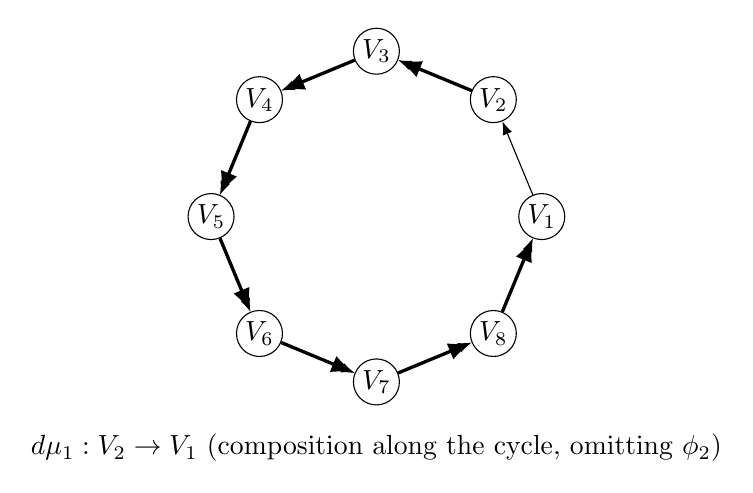
\begin{tikzpicture}[scale=1.05, every node/.style={circle,draw,inner sep=1.2pt}, >=Latex]
        % vertices on a circle
        \def\R{2.0}
        \foreach \i in {1,...,8} {
            \node (v\i) at ({\R*cos(360*(\i-1)/8)},{\R*sin(360*(\i-1)/8)}) {$V_{\i}$};
        }
        % cycle arrows
        \foreach \i [evaluate=\i as \j using {int(mod(\i,8)+1)}] in {1,...,8} {
            \draw[->] (v\i) -- (v\j);
        }
        % highlight a representative path for d\mu_l
        \draw[->,very thick] (v2) -- (v3);
        \draw[->,very thick] (v3) -- (v4);
        \draw[->,very thick] (v4) -- (v5);
        \draw[->,very thick] (v5) -- (v6);
        \draw[->,very thick] (v6) -- (v7);
        \draw[->,very thick] (v7) -- (v8);
        \draw[->,very thick] (v8) -- (v1);
        \node[draw=none,rectangle] at (0,-2.8) {$d\mu_{1}: V_2\to V_1$ (composition along the cycle, omitting $\phi_2$)};
    \end{tikzpicture}
    \caption{The cyclic quiver $C_n$ (illustrated here with $n=8$). The thick arrows indicate the path whose composition gives a typical $d\mu_l$ map along the cycle (example: $d\mu_{2}:V_2\to V_1$).}
\end{figure}

\begin{proposition}[Equivariance of the cyclic composition maps]\label{prop:mu-equivariant}
Let $C_{L+1}$ be the cyclic quiver on vertices $\{0,\ldots,L\}$, let $\mathrm{Rep}_{d}(C_{L+1})$ be its representation space with
$V_l\cong\mathbb{R}^{d_l-r}$, and let
\[\phi=(\phi_1,\ldots,\phi_L,\phi_{L+1})\in \Rep_d(C_{L+1}).\]
Define the base--change group
\[
G_d:=\prod_{l=0}^{L} \mathrm{GL}(V_l)
\]
acting on $\mathrm{Rep}_{d}(C_{L+1})$ via
\[
(g\cdot \phi)_l := g_l\,\phi_l\,g_{l-1}^{-1},\quad (l=0,\ldots,L), \ \text{mod} \ L+1
\]
For each $l=1,\ldots,L$, define
\[
d\mu_l(\phi) := \phi_{l-1}\cdots\phi_1\,\phi_{L+1}\,\phi_L\cdots\phi_{l+1}\in\mathrm{Hom}(V_{l+1},V_l),
\]
with the convention that an empty product is the identity.
Then, for all $g\in G_d$ and all $l=0,\ldots,L$,
\[
d\mu_l(g\cdot \phi) = g_l\,d\mu_l(\phi)\,g_{l+1}^{-1}.
\]
\end{proposition}

\begin{proof}
Expand $d\mu_l(g\cdot\phi)$ as a product of the maps $(g\cdot\phi)_i$. Each factor contributes a left multiplication by some $g_i$ and a right multiplication by $g_{i+1}^{-1}$, and all intermediate terms cancel by associativity, leaving only $g_l$ on the left and $g_{l+1}^{-1}$ on the right.
\end{proof}

\begin{proposition}[Orbit decomposition of $\Gamma_d$]\label{prop:GammaC-orbits}
Let
\[
\Gamma_d:=\Big\{\phi\in \mathrm{Rep}_{d}(C_{L+1})\ \Big|\ d\mu_l(\phi)=0\ \text{for all }l=1,\ldots,L\Big\}.
\]
Then $\Gamma_d$ is $G_d$-invariant. In particular, $\Gamma_d$ decomposes as a disjoint union of $G_d$-orbits:
\[
\Gamma_d = \bigsqcup_{\phi\in \Gamma_d} G_d\cdot \phi.
\]
\end{proposition}

\begin{proof}
By Proposition~\ref{prop:mu-equivariant}, each map $d\mu_l$ is $G_d$-equivariant and hence the vanishing set $d\mu_l^{-1}(0)$ is $G_d$-stable. Intersecting over $l=1,\ldots,L$ shows that $\Gamma_d$ is $G_d$-stable. Any group action partitions a set into disjoint orbits, yielding the stated decomposition.
\end{proof}
Note that $\Gamma_d\cong \Rep_d(C_{L+1})/< d\mu_l > $ is then finite dimensional and we can clasified indecomposable using indecomposable representations of Nakayama algebras.
\subsection{Cyclic quiver as a bounded module}
\begin{definition}[Path algebra]
Let $Q$ be a quiver. The \emph{path algebra} $kQ$ is the $k$-vector space with basis given by all directed paths in $Q$ (including the trivial paths $e_i$ of length $0$ at each vertex $i$), with multiplication given by concatenation of composable paths and $0$ otherwise, extended by bilinearity.
\end{definition}

\begin{definition}[Bound quiver algebra associated with $\Gamma_d$]
Let $Q=C_{L+1}$ and for each $l=0,\ldots,L$ let $p_l\in kQ$ be the path
\[
 p_l := a_{l-1}\cdots a_1\,a_{L+1}\cdots a_{l+1},
\]
interpreting empty products as the corresponding trivial path.
Let $I\subset kQ$ be the two-sided ideal generated by $\{p_1,\ldots,p_{L}\}$.
The quotient algebra
\[
A:=kQ/I
\]
is called the \emph{bound quiver algebra} associated with these relations.
\end{definition}

\begin{definition}[Representation of an algebra of dimension $d$]
Let $A$ be a $k$-algebra and let $d=(d_0,\ldots,d_L)$.
A \emph{representation of $A$ of dimension $d$ compatible with the vertices} is a left $A$-module structure on
$V:=\bigoplus_{i=0}^L k^{d_i}$ such that the idempotents $e_i\in kQ\twoheadrightarrow A$ act as the projections onto the $i$-th summand.
We denote the corresponding representation space by $\mathrm{Rep}_d(A)$.
\end{definition}

\begin{proposition}[From quiver representations with relations to $A$-modules]
There is a well-defined map
\[
F:\Gamma_d\to \mathrm{Rep}_d(A)
\]
which sends $\phi\in\Gamma_d$ to the unique $A$-module structure on $V$ for which each arrow $a_i$ acts by the linear map $\phi_i$.
\end{proposition}

\begin{proof}
Given $\phi\in\Gamma_d$, the tuple of linear maps $(\phi_i)_i$ defines a representation of the quiver $Q=C_{L+1}^{op}$, hence a left $kQ$-module structure on $V$ by letting a path act by the corresponding composition of arrow maps.
For each $l$, the defining condition $\mu_l(\phi)=0$ is exactly the statement that the element $p_l\in kQ$ acts as the zero map on $V$.
Since $I$ is the two-sided ideal generated by the $p_l$, every element of $I$ also acts by zero.
Therefore the $kQ$-action factors through the quotient $A=kQ/I$, producing a unique $A$-module structure on $V$ with the required arrow actions.
\end{proof}

\begin{proposition}[From $A$-modules to quiver representations with relations]
There is a well-defined map
\[
G:\mathrm{Rep}_d(A)\to \Gamma_d
\]
which sends an $A$-module structure on $V$ to the induced quiver representation $\phi$ whose arrow maps are the actions of the classes of the arrows $a_i$.
\end{proposition}

\begin{proof}
Let $V$ be a representation in $\mathrm{Rep}_d(A)$.
Composing the action map $A\to \mathrm{End}_k(V)$ with the quotient map $kQ\twoheadrightarrow A$ gives a $kQ$-module structure on $V$.
Restricting the action of each arrow basis element $a_i$ to the appropriate vertex summand yields linear maps $\phi_i:V_i\to V_{i+1}$ and hence a point $\phi\in\mathrm{Rep}_d(C_n)$.
Because each $p_l$ maps to zero in $A$, it acts as the zero endomorphism on $V$.
Equivalently, the composed linear map $\mu_l(\phi)$ is zero for every $l$, so $\phi\in\Gamma_d$.
\end{proof}

\begin{proposition}[Correspondence between $\Gamma_d$ and $\mathrm{Rep}_d(A)$]
The maps $F$ and $G$ are mutually inverse bijections. In particular,
\[
\Gamma_d \cong \mathrm{Rep}_d(A),\qquad A=kQ/I.
\]
\end{proposition}

\begin{proof}
Starting from $\phi\in\Gamma_d$, the $A$-module $F(\phi)$ is by construction generated by the same arrow actions as $\phi$, so applying $G$ recovers the same tuple of arrow maps, hence $G(F(\phi))=\phi$.
Conversely, starting from an $A$-module structure on $V$, the map $G$ records the arrow actions and the map $F$ reconstructs the unique $A$-module whose arrow actions agree with those recorded, hence $F(G(V))=V$.
\end{proof}
\begin{lemma}[Finite-dimensionality of $A=kQ/I$]\label{lem:A-finite-dim}
Let $Q=C_{L+1}$ be the oriented cycle on $L+1$ vertices, and let $I\subset kQ$ be the two-sided ideal generated by the paths
$p_1,\dots,p_{L}$, where each $p_l$ is a path of length $L$ (the unique directed path going around the cycle while omitting one arrow).
Then every directed path in $Q$ of length $\ge L +1$ lies in $I$. In particular, $A=kQ/I$ is finite-dimensional.
\end{lemma}

\begin{proof}
Let $q$ be any directed path in $Q$ of length $\ge L+1$. Write $q=b_m b_{m-1}\cdots b_1$ as a concatenation of arrows with $m\ge L+1$.
Consider the contiguous subpath $q':=b_{L}\cdots b_1$ of length $L$. Since $Q$ is an oriented $L+1$-cycle, there is exactly one directed
path of length $L$ from its source to its target, hence $q'$ must coincide with one of the generators $p_l$.
Therefore $q=q''\,p_l$ for some (possibly trivial) path $q''$, so $q\in I$ because $I$ is a two-sided ideal.

Thus all paths of length $\ge L+1$ vanish in $A$, so $A$ is spanned by the residue classes of paths of length $<L+1$, a finite set. Hence $A$ is finite-dimensional.
\end{proof}

\subsection{Bounded modules are Nakayama algebras}
\begin{definition}[$A$-module]
Let $A$ be a (not necessarily commutative) $k$-algebra.
A (left) \emph{$A$-module} is a $k$-vector space $M$ together with a $k$-bilinear map
\[
A\times M\to M,\qquad (a,m)\mapsto a\cdot m,
\]
such that for all $a,b\in A$ and $m\in M$ one has
\[
(ab)\cdot m = a\cdot (b\cdot m),\qquad 1_A\cdot m = m.
\]
A \emph{homomorphism} of $A$-modules is a $k$-linear map commuting with the $A$-action.
\end{definition}

\begin{definition}[Indecomposable module]
An $A$-module $M$ is \emph{indecomposable} if $M\neq 0$ and there do not exist nonzero submodules $M_1,M_2\subset M$ such that
\[
M \cong M_1\oplus M_2.
\]
Equivalently, $M$ is indecomposable if every idempotent endomorphism of $M$ is either $0$ or $\mathrm{id}_M$.
\end{definition}

\begin{definition}[Composition series]
Let $M$ be a finite-dimensional $A$-module.
A \emph{composition series} of $M$ is a finite chain of submodules
\[
0=M_0\subset M_1\subset \cdots \subset M_{\ell}=M
\]
such that each successive quotient $M_i/M_{i-1}$ is \emph{simple}.
The integer $\ell$ is called the \emph{length} of the series.
\end{definition}

\begin{definition}[Projective module]
An $A$-module $P$ is \emph{projective} if for every surjective $A$-module homomorphism $f:M\twoheadrightarrow N$ and every $A$-module homomorphism $g:P\to N$, there exists an $A$-module homomorphism $\tilde g:P\to M$ such that $f\circ \tilde g=g$.
Equivalently, $P$ is projective if the functor $\mathrm{Hom}_A(P,-)$ is exact.
\end{definition}

\begin{definition}[Indecomposable projective module]
A \emph{projective indecomposable} $A$-module is an $A$-module that is both projective and indecomposable.
For a finite-dimensional basic algebra $A$, every indecomposable projective module is of the form $P_i\cong Ae_i$ for a primitive idempotent $e_i\in A$, and every projective module decomposes uniquely as a direct sum of indecomposable projectives.
\end{definition}

\begin{definition}[Uniserial module]
An $A$-module $M$ is \emph{uniserial} if it admits a unique composition series. Equivalently, the set of submodules of $M$ is totally ordered by inclusion.
\end{definition}
\begin{definition}[\textbf{Nakayama algebra}]
Let $A$ be a finite-dimensional $k$-algebra. We say that $A$ is a \emph{Nakayama algebra} if every indecomposable left $A$-module is \emph{uniserial}, i.e.\ it admits a unique composition series.
Equivalently, $A$ is Nakayama if every indecomposable projective left $A$-module is uniserial (and hence every indecomposable injective is uniserial).
\end{definition}

\begin{definition}[Admissible ideal]
Let $Q$ be a finite quiver and let $kQ$ be its path algebra. Write $(kQ)_{\ge m}$ for the $k$-span of all paths of length at least $m$.
A two-sided ideal $I\subset kQ$ is called \emph{admissible} if there exists an integer $m\ge 2$ such that
\[
(kQ)_{\ge m}\subseteq I \subseteq (kQ)_{\ge 2}.
\]
\end{definition}

\begin{definition}[Jacobson radical]
Let $A$ be a (not necessarily commutative) ring. The \emph{Jacobson radical} $J(A)$ is the intersection of all maximal left ideals of $A$.
If $A$ is a finite-dimensional $k$-algebra, then equivalently
\[
J(A)=\bigcap_{S\ \text{simple}} \ker\big(A\to \mathrm{End}_k(S)\big),
\]
i.e.\ $J(A)$ is the largest two-sided ideal that acts by zero on every simple $A$-module.
\end{definition}

\begin{proposition}[\textbf{Bound quiver criterion for Nakayama algebras}]\label{prop:bound-quiver-nakayama}
Let $A \simeq kQ/I$ be a finite-dimensional bound quiver algebra, where $Q$ is a finite quiver and
$I\subset kQ$ is an admissible ideal.
Assume that for every vertex $i\in Q_0$ there is at most one arrow leaving $i$ and at most one arrow entering $i$.
Then $A$ is a Nakayama algebra.

Moreover, if $Q$ is connected and has exactly one arrow leaving and exactly one arrow entering each vertex, then $Q$ is an oriented cycle and $A$ is a \emph{cyclic Nakayama algebra}. If instead $Q$ is connected and has a unique source and a unique sink, then $Q$ is an oriented line and $A$ is a \emph{linear Nakayama algebra}.
\end{proposition}

\begin{proof}
Let $e_i\in kQ\twoheadrightarrow A$ be the primitive idempotent corresponding to a vertex $i\in Q_0$, and consider the indecomposable projective module $P_i := Ae_i$.
As a $k$-vector space, $P_i$ is spanned by residue classes of paths in $Q$ starting at $i$ (modulo the relations in $I$).
Because there is at most one arrow leaving each vertex, for each $\ell\ge 0$ there is \emph{at most one} directed path of length $\ell$ starting at $i$; hence $P_i$ has a basis indexed by (the surviving classes of) these paths.

Let $J\subset A$ denote the Jacobson radical. Since $A\simeq kQ/I$ with $I$ admissible, $J$ is generated (as a two-sided ideal) by the classes of arrows, and one has
\[
J^\ell P_i = J^\ell Ae_i \ \cong\ (J^\ell)e_i,
\]
which is spanned by classes of paths of length $\ge \ell$ starting at $i$.
By the previous paragraph, for each $\ell$ the quotient $J^\ell P_i/J^{\ell+1}P_i$ is either $0$ or a simple module (it is spanned by the class of the unique surviving path of length $\ell$, if it exists).
Therefore the radical filtration
\[
P_i \supset JP_i \supset J^2P_i \supset \cdots
\]
is a chain whose successive quotients are simple (or zero), i.e.\ $P_i$ is uniserial.

Thus every indecomposable projective $P_i$ is uniserial, and hence $A$ is a Nakayama algebra.

For the final statements: if $Q$ is connected and every vertex has exactly one incoming and one outgoing arrow, then the underlying directed graph is a directed cycle. If $Q$ is connected and has a unique source and sink with all other vertices having one incoming and one outgoing arrow, then the directed graph is a directed line. These correspond to cyclic and linear Nakayama algebras respectively.
\end{proof}
\subsection{Cyclic monomial Nakayama algebra with uniform Kupisch series}
Throughout this subsection, let $Q=C_{L+1}$ be the oriented $L+1$-cycle, let $kQ$ be its path algebra, and let
\[
A:=kQ/I
\]
be the bound quiver algebra from Definition~(Bound quiver algebra associated with $\Gamma_d$).

\begin{definition}[Monomial (path) ideal / monomial algebra]
An ideal $I\subset kQ$ is called \emph{monomial} if it is generated (as a two-sided ideal) by paths in $Q$.
A quotient $kQ/I$ with $I$ monomial is called a \emph{monomial algebra}.
\end{definition}

\begin{definition}[Kupisch series]
Let $A$ be a finite-dimensional basic algebra with primitive idempotents $e_1,\ldots,e_{L+1}$ and indecomposable projectives
$P_i:=Ae_i$.
The \emph{Kupisch series} of $A$ is the $L+1$-tuple
\[
(c_1,\ldots,c_{L+1}),\qquad c_i:=\ell(P_i),
\]
where $\ell(P_i)$ denotes the composition length of $P_i$.
\end{definition}

\begin{remark}[Loewy length]
For a finite-dimensional algebra $A$ with Jacobson radical $J=J(A)$, the \emph{Loewy length} is the smallest integer $n$ such that $J^n=0$.
\end{remark}

\begin{proposition}[Identification and Kupisch series]
With $Q=C_{L+1}$ and $I=(p_1,\ldots,p_{L+1})$ as above, the algebra $A=kQ/I$ is a \emph{cyclic monomial Nakayama algebra}.
Moreover its Kupisch series is uniform:
\[
(c_1,\ldots,c_{L+1})=(L,\ldots,L).
\]
\end{proposition}

\begin{proof}
By construction, the ideal $I$ is generated by the paths $p_1,\ldots,p_{L+1}$, hence $I$ is monomial and $A$ is a monomial algebra.
By Proposition~\ref{prop:bound-quiver-nakayama}, $A$ is Nakayama; since $Q=C_{L+1}$ is an oriented cycle, $A$ is in fact \emph{cyclic} Nakayama.

Fix a vertex $i$ and consider $P_i=Ae_i$.
Modulo $I$, every path in $Q$ of length $\ge L$ starting at $i$ vanishes, while for each $t=0,1,\ldots,L-1$ there is exactly one directed path of length $t$ starting at $i$.
Therefore $P_i$ has a $k$-basis given by the residue classes of these $L$ paths (length $0$ through $L-1$).

Since $J=J(A)$ is generated by the classes of arrows (as recalled in the proof of Proposition~\ref{prop:bound-quiver-nakayama}), the radical filtration
\[
P_i \supset JP_i \supset J^2P_i \supset \cdots
\]
has successive quotients $J^tP_i/J^{t+1}P_i$ one-dimensional (hence simple) for $t=0,\ldots,L-1$, and zero thereafter.
Thus $\ell(P_i)=L$ for every $i$, which gives the Kupisch series $(L,\ldots,L)$.
\end{proof}

\begin{remark}
Equivalently, $A$ can be viewed as a \emph{truncated cycle algebra}: it is the path algebra of an oriented cycle with all paths of length $\ge L$ killed.
\end{remark}
\subsection{Indecomposable representations of Nakayama algebras}
\begin{definition}[The uniserial modules $M(i,\ell)$]
Fix $Q=C_{L+1}$ with vertices $Q_0=\{0,\dots,L\}$ and arrows $a_i:l-1\to l$ for $l=1,\dots,L$ and $a_{L+1}:L\to 0$.
For $i\in Q_0$ and $0\le \ell\le L$, define a representation $M(i,\ell)$ of $Q$ by
\[
M(i,\ell)_j :=
\begin{cases}
k, & j\in\{i,i+1,\dots,i+\ell-1\}\ (\mathrm{mod}\ L + 1),\\
0, & \text{otherwise},
\end{cases}
\]
and for each arrow $a_j:j-1\to j$,
\[
M(i,\ell)_{a_j} :=
\begin{cases}
\mathrm{id}_k, & \text{if both source and target are }k,\\
0, & \text{otherwise}.
\end{cases}
\]
\end{definition}

\begin{lemma}[The relations vanish on $M(i,\ell)$]\label{lem:Miell-well-defined}
Let $Q=C_{L+1}$ and, for each $l\in\{1,\dots,L+1\}$, let
\[
p_l := a_{l-1}\cdots a_1\, a_{L+1}\cdots a_{l+1}
\]
be the oriented path of length $L$ going once around the cycle and omitting $a_l$.
Set $A:=kQ/\langle p_1,\dots,p_{L+1}\rangle$.
Then, for every $i\in Q_0$ and $1\le \ell\le L$, the representation $M(i,\ell)$ factors through $A$, hence defines a finite-dimensional left $A$-module.
\end{lemma}

\begin{proof}
Fix $i$ and $\ell$. Each path $p_l$ has length $L$.
Since the support of $M(i,\ell)$ contains only $\ell\le L$ consecutive vertices, the corresponding composition along $p_l$ necessarily passes through a vertex where $M(i,\ell)$ is zero.
Therefore $p_l$ acts by the zero map on $M(i,\ell)$ for every $l$, so all generators of the ideal $\langle p_1,\dots,p_{L}\rangle$ act trivially.
Hence the $kQ$-action factors through $A$.
\end{proof}

\begin{lemma}[Uniseriality of $M(i,\ell)$]\label{lem:Miell-uniserial}
For every $i\in Q_0$ and $1\le \ell\le L + 1$, the $A$-module $M(i,\ell)$ is uniserial, and in particular indecomposable.
\end{lemma}

\begin{proof}
Any nonzero submodule $N\subseteq M(i,\ell)$ must contain the one-dimensional space at some vertex in the support.
Because all arrow maps inside the support are identities, containing a vertex forces $N$ to contain all vertices reachable along the directed arrows within the support.
Consequently, the nonzero submodules are exactly the modules
$M(i+t,\ell-t)$ for $t=0,\dots,\ell-1$ (indices taken modulo $n$), and they form a chain under inclusion.
Thus submodules are totally ordered and $M(i,\ell)$ is uniserial.
\end{proof}

\begin{lemma}[Endomorphisms of $M(i,\ell)$]\label{lem:Miell-end}
For every $i\in Q_0$ and $1\le \ell\le L$, one has $\mathrm{End}_A\big(M(i,\ell)\big)\cong k$.
\end{lemma}

\begin{proof}
Let $f\in \mathrm{End}_A(M(i,\ell))$.
On each vertex $j$ in the support, $f$ is multiplication by some scalar $\lambda_j\in k$.
For each arrow inside the support, the arrow map is $\mathrm{id}_k$, so commutativity forces $\lambda_{j+1}=\lambda_j$.
Hence all $\lambda_j$ coincide with a single scalar $\lambda$, and $f=\lambda\,\mathrm{id}$.
\end{proof}

\begin{lemma}[Projective truncations realize $M(i,\ell)$]\label{lem:Miell-as-truncation}
Let $P(i):=Ae_i$ be the indecomposable projective at vertex $i$ and let $J:=J(A)$.
Then, for every $i\in Q_0$ and $1\le \ell\le L$, there is an isomorphism of $A$-modules
\[
P(i)/J^{\ell}P(i)\ \cong\ M(i,\ell).
\]
\end{lemma}

\begin{proof}
By Proposition~\ref{prop:bound-quiver-nakayama} and the previous subsection, $A$ is a cyclic Nakayama algebra with uniform Kupisch series $(L,\ldots,L)$.
In particular, $P(i)$ is uniserial of length $L$, and $J^tP(i)$ is spanned by residue classes of paths of length $\ge t$ starting at $i$.
Thus $P(i)/J^{\ell}P(i)$ has a basis given by the residue classes of the unique paths of lengths $0,1,\dots,\ell-1$ starting at $i$.
Under the induced quiver description, this quotient has one-dimensional spaces on the vertices $i,i+1,\dots,i+\ell-1$ (mod $L+1$) and identity maps along arrows inside the support, which is exactly $M(i,\ell)$.
\end{proof}

\begin{proposition}[Indecomposable representations of the cyclic truncated Nakayama algebra]
\label{prop:indecomp-cyclic-nakayama}
Let $Q=C_{L+1}$ be the oriented cyclic quiver with arrows $a_i:i\to i+1$ for $i=1,\dots,L$ and $a_{L+1}:L\to 0$.
For each $l\in\{1,\dots,L+1\}$, let $p_l$ be the path of length $L$ going once around the cycle and omitting $a_l$, and set
\[
A := kQ / \langle p_1,\dots,p_{L+1}\rangle.
\]
Then every finite-dimensional indecomposable left $A$-module is isomorphic to a unique module $M(i,\ell)$ with $i\in Q_0$ and $1\le \ell\le L$.
Equivalently, every indecomposable $A$-module is of the form $P(i)/J^{\ell}P(i)$ for a unique pair $(i,\ell)$.
In particular, $A$ has exactly $(L+1)L$ indecomposable modules up to isomorphism.
\end{proposition}

\begin{proof}
By Lemma~\ref{lem:Miell-well-defined}, each $M(i,\ell)$ is a well-defined finite-dimensional $A$-module, and by Lemma~\ref{lem:Miell-uniserial} it is indecomposable.

Conversely, since $A$ is Nakayama (Proposition~\ref{prop:bound-quiver-nakayama}), every indecomposable $A$-module is uniserial and hence a quotient of a unique indecomposable projective $P(i)=Ae_i$.
Its composition length is some $\ell$ with $1\le \ell\le \ell(P(i))=L$, and uniseriality forces the quotient to be $P(i)/J^{\ell}P(i)$.
By Lemma~\ref{lem:Miell-as-truncation}, this module is isomorphic to $M(i,\ell)$.

Uniqueness follows because the top simple module determines $i$ and the length determines $\ell$.
Counting pairs $(i,\ell)$ with $i\in Q_0$ and $1\le \ell\le L$ gives $(L+1)L$.
\end{proof}
More details about this can be found in the following lecture notes:
\href{https://www.math.uni-bielefeld.de/~wcrawley/1920noncommalg2/NA2.pdf}{Noncommutative Algebra 2: Representations of finite-dimensional algebras} in particular theorem and corroloray section 1.6.
We have a Krull schmidt theorem for these Nakayama algebras.
\begin{proposition}[Krull--Schmidt for the cyclic truncated Nakayama algebra]\label{prop:KS-cyclic-truncated-nakayama}
Let $A=kQ/I$ be the cyclic truncated Nakayama algebra, where $Q=C_{L+1}$ is the oriented $L+1$-cycle and $I$ is the ideal generated by the length-$(L)$ paths $p_1,\dots,p_{L+1}$ (equivalently, all paths of length $\ge L+1$ vanish in $A$).
Let $\mathrm{mod}\text{-}A$ denote the category of finite-dimensional left $A$-modules.
Then every $M\in \mathrm{mod}\text{-}A$ admits a decomposition as a finite direct sum of indecomposable $A$-modules.
Moreover, this decomposition is unique up to reordering and isomorphism of the indecomposable summands.
Equivalently, using the explicit indecomposables $M(i,\ell)$ from Proposition~\ref{prop:indecomp-cyclic-nakayama}, there exist uniquely determined multiplicities
$m_{i,\ell}\in\mathbb{Z}_{\ge 0}$ such that
\[
M \ \cong\ \bigoplus_{i=0}^{L} \ \bigoplus_{\ell=1}^{L} \ M(i,\ell)^{\oplus m_{i,\ell}}.
\]
\end{proposition}

\begin{proof}[Proof sketch]
Since $A$ is finite-dimensional over $k$, it is left artinian (and left noetherian), hence every object of $\mathrm{mod}\text{-}A$ has finite length.
In particular, $\mathrm{mod}\text{-}A$ is a Krull--Schmidt category: every object decomposes as a finite direct sum of indecomposables, and such a decomposition is unique up to permutation and isomorphism.

Concretely, existence follows by choosing a nonzero module $M$ and repeatedly splitting off a nontrivial direct summand until all summands are indecomposable; the process terminates because $M$ has finite length.
Uniqueness follows because each indecomposable has a local endomorphism ring (for example, by Lemma~\ref{lem:Miell-end} in the explicit classification), and the classical Krull--Schmidt--Azumaya argument applies.

Finally, Proposition~\ref{prop:indecomp-cyclic-nakayama} classifies the indecomposables as the modules $M(i,\ell)$, so any Krull--Schmidt decomposition can be rewritten uniquely in the stated multiplicity form.
\end{proof}
\textbf{Note}: This enables to parameterize the orbits of $\Gamma$ with the indecomposables representations.
\paragraph{Orbits, isomorphism classes, and multiplicity patterns.}
Fix a finite-dimensional $k$-algebra $A$ and a dimension vector $d=(d_0,\dots,d_{L})$.
Recall that
\[
\mathrm{Rep}_d(A)
=\Big\{\text{left $A$-module structures on }V=\bigoplus_{i=0}^{L} k^{d_i}\text{ such that each idempotent $e_i$ acts as the projection onto }k^{d_i}\Big\}.
\]
Let
\[
G_d:=\prod_{i=0}^{L} \mathrm{GL}(k^{d_i})
\]
act on $\mathrm{Rep}_d(A)$ by \emph{change of bases at the vertices} (equivalently, by transport of structure):
for $g=(g_0,\dots,g_L)\in G_d$ and a module structure $\rho:A\to \mathrm{End}_k(V)$, define a new module
structure $g\cdot \rho$ by
\[
(g\cdot \rho)(a)\;:=\; g\,\rho(a)\,g^{-1},\qquad g:=\bigoplus_{i=1}^n g_i\in \mathrm{GL}(V).
\]
When $A\simeq kQ/I$ is presented as a bound quiver algebra, this action is equivalently given on arrow
maps by $(g\cdot \phi)_a=g_{t(a)}\,\phi_a\,g_{s(a)}^{-1}$.
Then two points $\rho,\rho'\in \mathrm{Rep}_d(A)$ lie in the same $G_d$-orbit if and only if the corresponding
$A$-modules $(V,\rho)$ and $(V,\rho')$ are isomorphic in $\mathrm{mod}\text{-}A$.
Consequently, there is a canonical bijection
\[
\big(G_d\backslash \mathrm{Rep}_d(A)\big)\ \cong\ \Big\{\text{isomorphism classes of $A$-modules $M$ with $\dim(e_iM)=d_i$ for all $i$}\Big\}.
\]

Now specialize to the cyclic truncated Nakayama algebra $A=kQ/I$ considered above.
Its indecomposable modules are the uniserials $M(i,\ell)$ with $i\in\{0,\dots,L\}$ (indices taken modulo $L+1$) and $1\le \ell\le L$
(Proposition~\ref{prop:indecomp-cyclic-nakayama}).
By the Krull--Schmidt theorem (Proposition~\ref{prop:KS-cyclic-truncated-nakayama}), every finite-dimensional
$A$-module $M$ admits a decomposition
\[
M\ \simeq\ \bigoplus_{i=0}^{L}\ \bigoplus_{\ell=1}^{L} M(i,\ell)^{\oplus m_{i,\ell}},
\qquad m_{i,\ell}\in\mathbb{Z}_{\ge 0},
\]
and this decomposition is unique up to permutation of summands.
The multiplicities $(m_{i,\ell})$ determine (and are constrained by) the dimension vector $d$ via the \emph{covering equations}
\begin{equation}\label{eq:cyclic-multiplicity-constraints}
d_k \;=\; \sum_{i=0}^{L}\ \sum_{\ell=1}^{L} m_{i,\ell}\,\mathbf{1}\!\left\{k\in\{i,i+1,\dots,i+\ell-1\}\ (\mathrm{mod}\ L+1)\right\},
\qquad k=0,\dots,L,
\end{equation}
since $M(i,\ell)$ contributes a one-dimensional space at vertex $k$ exactly when $k$ lies in its cyclic
support interval of length $\ell$ starting at $i$.
Define the set of \emph{multiplicity patterns}
\[
M_d^{+}(A)
:=\left\{(m_{i,\ell})\in \mathbb{Z}_{\ge 0}^{L(L+1)}\ \middle|\ \text{\eqref{eq:cyclic-multiplicity-constraints} holds for all }k\right\}.
\]
Then the above discussion yields a concrete parametrization of orbits:
every $G_d$-orbit in $\mathrm{Rep}_d(A)$ corresponds to a unique isomorphism class in $\mathrm{mod}\text{-}A$,
and hence to a unique multiplicity pattern $(m_{i,\ell})\in M_d^{+}(A)$ via its Krull--Schmidt decomposition.
In other words, we obtain canonical bijections
\[
G_d\backslash \mathrm{Rep}_d(A)
\ \cong\
\Big\{\text{isomorphism classes in $\mathrm{mod}\text{-}A$ with dimension vector $d$}\Big\}
\ \cong\
M_d^{+}(A),
\]
where the last map sends an $A$-module to the multiplicities of the indecomposables $M(i,\ell)$ in its Krull--Schmidt decomposition.
\begin{proposition}[Orbit stratification of $\Gamma_d$ by indecomposable Nakayama modules]
\label{prop:Gamma_orbit_stratification}

Fix $L \ge 1$ and let $Q = C_{L+1}$ be the oriented cyclic quiver on vertices
$\{0,\dots,L\}$.  
Let $A := kQ/I$ be the bound quiver algebra, where $I$ is the ideal generated by the length-$L$
paths $p_1,\dots,p_{L+1}$ obtained by going once around the cycle and omitting one arrow.
Let $d=(d_0,\dots,d_L)$ be a dimension vector.

Define
\[
\Gamma_d := \left\{
\phi \in \mathrm{Rep}_d(Q)
\;\middle|\;
d\mu_\ell(\phi)=0 \text{ for all } \ell=1,\dots,L
\right\},
\]
where
\[
d\mu_\ell(\phi) := \phi_{\ell-1}\cdots \phi_1\,\phi_{L+1}\,\phi_L\cdots \phi_{\ell+1}.
\]

Let
\[
G_d := \prod_{i=0}^{L} \mathrm{GL}(k^{d_i})
\]
act on $\Gamma_d$ by base change at the vertices.

\medskip

Then the following hold.

\begin{enumerate}
\item
There is a canonical identification
\[
\Gamma_d \;\cong\; \mathrm{Rep}_d(A),
\]
under which the $G_d$-action coincides with transport of structure on $A$-modules.

\item
The algebra $A$ is a finite-dimensional cyclic Nakayama algebra.  
Its indecomposable finite-dimensional left modules are, up to isomorphism, the uniserial modules
\[
M(i,\ell), \qquad i \in \{0,\dots,L\}, \quad 1 \le \ell \le L,
\]
supported on $\ell$ consecutive vertices starting at $i$ (indices taken modulo $L+1$).

\item
Every $A$-module $M$ of dimension vector $d$ admits a unique (up to permutation)
Krull--Schmidt decomposition
\[
M \;\cong\; \bigoplus_{i=0}^{L}\;\bigoplus_{\ell=1}^{L} M(i,\ell)^{\oplus m_{i,\ell}},
\]
for uniquely determined multiplicities $m_{i,\ell} \in \mathbb{Z}_{\ge 0}$ satisfying the
dimension constraints
\[
d_k \;=\;
\sum_{i=0}^{L}\sum_{\ell=1}^{L}
m_{i,\ell}\,
\mathbf{1}\!\left\{
k \in \{i,i+1,\dots,i+\ell-1\} \ (\mathrm{mod}\ L+1)
\right\},
\quad k=0,\dots,L.
\]

Denote by $\mathcal M_d^+(A)$ the finite set of all such multiplicity patterns
$m=(m_{i,\ell})$.

\item
For each $m \in \mathcal M_d^+(A)$, define the stratum
\[
\Gamma_d^{(m)}
:=
\left\{
\phi \in \Gamma_d
\;\middle|\;
F(\phi) \cong
\bigoplus_{i,\ell} M(i,\ell)^{\oplus m_{i,\ell}}
\right\},
\]
where $F(\phi)$ denotes the associated $A$-module.

Then $\Gamma_d^{(m)}$ is a single $G_d$-orbit.

\item
The variety $\Gamma_d$ decomposes as a disjoint union of these orbits:
\[
\Gamma_d
\;=\;
\bigsqcup_{m \in \mathcal M_d^+(A)} \Gamma_d^{(m)}
\;=\;
\bigsqcup_{m \in \mathcal M_d^+(A)} G_d \cdot \phi_m,
\]
where $\phi_m$ is any representative whose associated $A$-module has multiplicity pattern $m$.
\end{enumerate}

\noindent
In particular, the $G_d$-orbits in $\Gamma_d$ are canonically parameterized by the
multiplicity data of indecomposable $A$-modules, i.e.\ by the set
$\mathcal M_d^+(A)$.
\end{proposition}



\section{Stratification of $\Gamma_{XY}$}
While the indecomposable representation of $\Gamma$ are parameterized by the $M(i,\ell)$ from the previous modules over Nakayama algebras we are actually interested in decomposing:
\begin{equation*}
    \Gamma_{\sigma} := \left\{(\phi_1,\ldots,\phi_{L+1})\in \mathrm{Rep}_d(C_{L+1})\;\middle|\; \phi_{l-1}\cdots\phi_1\,\phi_{L+1}\,\phi_L\cdots\phi_{l+1} = 0,\; \phi_{L+1}=\sigma\right\}.
\end{equation*}
where the map $\sigma\in \mathrm{Hom}(V_L,V_0)$ is fixed (in DLN it is $\Sigma_{XY}U_Q$).
The map
\begin{equation*}
    d\mu_{l,\sigma} := \phi_{l-1}\cdots\phi_1\,\sigma\,\phi_L\cdots\phi_{l+1}
\end{equation*}
is no longer $G_d$-equivariant.

\begin{definition}[Stabilizer group of the fixed arrow]\label{def:stabilizer-sigma}
Let $\sigma\in\mathrm{Hom}(V_L,V_0)$ be fixed. Define
\[
\mathrm{Stab}(\sigma):=\{(g_0,g_L)\in \mathrm{GL}(V_0)\times \mathrm{GL}(V_L)\mid g_0\,\sigma\,g_L^{-1}=\sigma\},
\]
and the corresponding subgroup of the base--change group
\[
G_\sigma:=\{g=(g_0,\ldots,g_L)\in \prod_{l=0}^L\mathrm{GL}(V_l)\mid (g_0,g_L)\in \mathrm{Stab}(\sigma)\}.
\]
\end{definition}

\begin{proposition}[$G_\sigma$-equivariance of the cyclic composition maps]\label{prop:mu-sigma-equivariant}
Fix $\sigma\in\mathrm{Hom}(V_L,V_0)$ and consider the representation space with $\phi_{L+1}=\sigma$.
For $\phi=(\phi_1,\ldots,\phi_L,\sigma)$ and each $l=1,\ldots,L$, define
\[
d\mu_{l,\sigma}(\phi):=\phi_{l-1}\cdots \phi_1\,\sigma\,\phi_L\cdots \phi_{l+1}\in\mathrm{Hom}(V_{l+1},V_l),
\]
with the convention that an empty product is the identity.
Then, for all $g\in G_\sigma$ and all $l$,
\[
d\mu_{l,\sigma}(g\cdot \phi)= g_l\,\mu_{l,\sigma}(\phi)\,g_{l+1}^{-1}.
\]
In particular, the subset $\Gamma_\sigma:=\bigcap_{l=1}^L d\mu_{l,\sigma}^{-1}(0)$ is $G_\sigma$-invariant.
\end{proposition}

\begin{proof}
Expand $d\mu_{l,\sigma}(g\cdot\phi)$ as a product of the maps $(g\cdot\phi)_i$.
All intermediate base-change factors cancel. The only remaining factors are $g_l$ on the left and
$g_{l+1}^{-1}$ on the right. The middle arrow is $(g\cdot\phi)_{L+1}=g_1\sigma g_L^{-1}$, which equals
$\sigma$ because $g\in G_\sigma$. 
\end{proof}
For all modules in $\Gamma_\sigma$ Krull-Schmidt applies (as a category of $A$-modules where $A$ is finite dimensional). We want to parameterize the orbits of $\Gamma_\sigma$ under the action of $G_\sigma$ and study their geometry (e.g. codimension).
\begin{lemma}[Intersection of a $G_d$--orbit with a fixed--arrow fiber]
\label{lem:orbit_fiber_intersection}
Let $L\ge 2$ and let $V_0,\dots,V_L$ be finite--dimensional vector spaces over an algebraically closed field $\Bbbk$.  
Set
\[
G_d \;:=\; \prod_{i=0}^L GL(V_i).
\]
Let $\Gamma_d$ be an affine variety equipped with an algebraic action of $G_d$.  
Assume there exists a morphism
\[
F:\Gamma_d \longrightarrow \Hom(V_L,V_0)
\]
satisfying the equivariance property
\begin{equation}
\label{eq:equivariance}
F(g\cdot x) \;=\; g_0\,F(x)\,g_L^{-1}
\qquad
\text{for all } g=(g_0,\dots,g_L)\in G_d,\; x\in\Gamma_d .
\end{equation}

Fix $\sigma\in \Hom(V_L,V_0)$ and define the fiber
\[
\Gamma_\sigma \;:=\; F^{-1}(\sigma).
\]
Define the stabilizer subgroup
\[
G_\sigma \;:=\; \{ g=(g_0,\dots,g_L)\in G_d \mid g_0\,\sigma\,g_L^{-1}=\sigma \}.
\]
Let $\mathcal O\subset \Gamma_d$ be a single $G_d$--orbit.  
Then either $\mathcal O\cap\Gamma_\sigma=\varnothing$, or else for every
$x\in\mathcal O\cap\Gamma_\sigma$ one has
\[
\mathcal O\cap\Gamma_\sigma \;=\; G_\sigma\cdot x .
\]
In particular, whenever $\mathcal O\cap\Gamma_\sigma\neq\varnothing$, this
intersection consists of a single $G_\sigma$--orbit.
\end{lemma}

\begin{proof}
We proceed in several steps.

\medskip\noindent
\textbf{Step 1: $\Gamma_\sigma$ is stable under the action of $G_\sigma$.}

Let $x\in\Gamma_\sigma$, so by definition $F(x)=\sigma$.  
Let $g\in G_\sigma$. Using the equivariance property \eqref{eq:equivariance},
\[
F(g\cdot x)
\;=\;
g_1\,F(x)\,g_L^{-1}
\;=\;
g_1\,\sigma\,g_L^{-1}.
\]
Since $g\in G_\sigma$, we have $g_1\,\sigma\,g_L^{-1}=\sigma$, and hence
$F(g\cdot x)=\sigma$. Therefore $g\cdot x\in\Gamma_\sigma$.  
This shows that $\Gamma_\sigma$ is invariant under the action of $G_\sigma$ and,
in particular,
\[
G_\sigma\cdot x \subseteq \Gamma_\sigma
\qquad
\text{for all } x\in\Gamma_\sigma .
\tag{$\ast$}
\]

\medskip\noindent
\textbf{Step 2: If $x\in\mathcal O\cap\Gamma_\sigma$, then
$G_\sigma\cdot x\subseteq \mathcal O\cap\Gamma_\sigma$.}

Let $x\in\mathcal O\cap\Gamma_\sigma$.  
Since $\mathcal O$ is a $G_d$--orbit, it is stable under the action of $G_d$ and
hence under the subgroup $G_\sigma\subseteq G_d$. Thus $G_\sigma\cdot x\subseteq
\mathcal O$.  
By $(\ast)$, $G_\sigma\cdot x\subseteq \Gamma_\sigma$.  
Combining these two inclusions gives
\[
G_\sigma\cdot x \subseteq \mathcal O\cap\Gamma_\sigma .
\tag{$\ast\ast$}
\]

\medskip\noindent
\textbf{Step 3: Any two points of $\mathcal O\cap\Gamma_\sigma$ differ by the
action of $G_\sigma$.}

Assume $x,y\in\mathcal O\cap\Gamma_\sigma$.  
Because $x$ and $y$ lie in the same $G_d$--orbit $\mathcal O$, there exists
$g=(g_1,\dots,g_L)\in G_d$ such that
\[
y = g\cdot x .
\]
Applying $F$ and using \eqref{eq:equivariance}, we obtain
\[
F(y)
\;=\;
F(g\cdot x)
\;=\;
g_1\,F(x)\,g_L^{-1}.
\]
Since $x,y\in\Gamma_\sigma$, we have $F(x)=F(y)=\sigma$. Therefore
\[
\sigma = g_1\,\sigma\,g_L^{-1}.
\]
By definition of $G_\sigma$, this implies $g\in G_\sigma$. Hence
$y=g\cdot x\in G_\sigma\cdot x$, and we conclude that
\[
\mathcal O\cap\Gamma_\sigma \subseteq G_\sigma\cdot x .
\tag{$\ast\ast\ast$}
\]

\medskip\noindent
\textbf{Step 4: Conclusion.}

If $\mathcal O\cap\Gamma_\sigma=\varnothing$, there is nothing to prove.
Otherwise choose any $x\in\mathcal O\cap\Gamma_\sigma$.  
Inclusion $(\ast\ast)$ gives $G_\sigma\cdot x\subseteq \mathcal O\cap\Gamma_\sigma$,
while inclusion $(\ast\ast\ast)$ gives the reverse inclusion. Therefore
\[
\mathcal O\cap\Gamma_\sigma = G_\sigma\cdot x .
\]
This proves that whenever the intersection is not empty, it consists of a single
$G_\sigma$--orbit. The lemma follows.
\end{proof}
\begin{proposition}[Rank label for Nakayama orbits and the fiber non-emptiness criterion over $\mathbb{R}$]
\label{prop:rank_label_and_nonemptiness_real}
Fix $L\ge 2$ and finite-dimensional real vector spaces $V_1,\dots,V_L$.
Let
\[
G_d \;:=\; \prod_{i=0}^L GL(V_i)
\qquad\text{and}\qquad
W \;:=\; \Hom_{\mathbb{R}}(V_L,V_0).
\]
Let $\Gamma_d$ be a real algebraic variety equipped with an algebraic action of $G_d$.
Assume there is a morphism of real varieties
\[
F:\Gamma_d \longrightarrow W
\]
satisfying the equivariance identity
\begin{equation}
\label{eq:equivariance_F}
F\!\big((g_0,\dots,g_L)\cdot x\big)=g_0\,F(x)\,g_L^{-1}
\qquad\text{for all } (g_0,\dots,g_L)\in G_d,\; x\in \Gamma_d .
\end{equation}

\medskip
\noindent
\textbf{Definition (Orbit label and rank label).}
Assume $\Gamma_d$ admits a decomposition into $G_d$--orbits indexed by a parameter set $\Lambda$,
\[
\Gamma_d \;=\; \bigsqcup_{\lambda\in\Lambda}\, \mathcal O_\lambda,
\]
where $\mathcal O_\lambda$ denotes the $G_d$--orbit corresponding to $\lambda$ (in the applications of this paper, $\lambda$ encodes the Krull--Schmidt multiplicities of the Nakayama indecomposables).  
For each $\lambda\in\Lambda$, define the integer
\begin{equation}
\label{eq:def_r_lambda}
r(\lambda) \;:=\; \mathrm{rank}\big(F(x)\big)\quad \text{for any } x\in \mathcal O_\lambda.
\end{equation}

\medskip
\noindent
Then the following statements hold.

\begin{enumerate}
\item[(i)] The integer $r(\lambda)$ in \eqref{eq:def_r_lambda} is well-defined, i.e.\ it does not depend on the choice of $x\in \mathcal O_\lambda$.
\item[(ii)] Fix $\sigma\in W$ and define the fiber $\Gamma_\sigma:=F^{-1}(\sigma)$. Then for every $\lambda\in\Lambda$,
\begin{equation}
\label{eq:nonemptiness}
\mathcal O_\lambda\cap \Gamma_\sigma \neq \varnothing
\qquad\Longleftrightarrow\qquad
r(\lambda)=\mathrm{rank}(\sigma).
\end{equation}
\end{enumerate}
\end{proposition}

\begin{proof}
We prove (i) and (ii) in separate steps.

\medskip\noindent
\textbf{Step 1: A basic invariance identity for ranks under left--right change of bases.}
Let $A\in GL(V_0)$, $B\in GL(V_L)$, and $T\in W=\Hom_{\mathbb{R}}(V_L,V_0)$.
Consider the map $T':=A\,T\,B^{-1}\in W$.
We have $\mathrm{rank}(T')=\mathrm{rank}(T)$.

\medskip\noindent
\textbf{Step 2: Proof of (i) (well-definedness of $r(\lambda)$).}
Fix $\lambda\in\Lambda$ and choose two points $x,y\in \mathcal O_\lambda$.
By definition of orbit, there exists $g=(g_0,\dots,g_L)\in G_d$ such that
\[
y=g\cdot x.
\]
Apply $F$ to both sides and use the equivariance identity \eqref{eq:equivariance_F}:
\[
F(y)=F(g\cdot x)=g_0\,F(x)\,g_L^{-1}.
\]
Now apply Step 1 with $A=g_0$, $B=g_L$, and $T=F(x)$. This yields
\[
\mathrm{rank}(F(y))=\mathrm{rank}(g_0\,F(x)\,g_L^{-1})=\mathrm{rank}(F(x)).
\]
Thus the rank of $F(\,\cdot\,)$ is constant along $\mathcal O_\lambda$, so the integer $r(\lambda)$
defined by \eqref{eq:def_r_lambda} is independent of the choice of $x\in\mathcal O_\lambda$.
This proves (i).

\medskip\noindent
\textbf{Step 3: A real classification fact for linear maps by rank.}
Let $S,T\in W=\Hom_{\mathbb{R}}(V_L,V_1)$. We use the following statement:

\smallskip\noindent
\emph{Claim.} If $\mathrm{rank}(S)=\mathrm{rank}(T)$, then there exist $A\in GL(V_1)$ and $B\in GL(V_L)$ such that
\begin{equation}
\label{eq:rank_equivalence}
S=A\,T\,B^{-1}.
\end{equation}

\medskip\noindent
\textbf{Step 4: Proof of (ii), forward implication.}
Assume $\mathcal O_\lambda\cap \Gamma_\sigma\neq \varnothing$.
Choose $x\in \mathcal O_\lambda\cap \Gamma_\sigma$.
By definition of $\Gamma_\sigma=F^{-1}(\sigma)$ we have $F(x)=\sigma$, hence
\[
\mathrm{rank}(\sigma)=\mathrm{rank}(F(x)).
\]
By definition of $r(\lambda)$ (and Step 2), $\mathrm{rank}(F(x))=r(\lambda)$ for any $x\in\mathcal O_\lambda$.
Therefore $\mathrm{rank}(\sigma)=r(\lambda)$, proving the forward direction of \eqref{eq:nonemptiness}.

\medskip\noindent
\textbf{Step 5: Proof of (ii), reverse implication.}
Assume $r(\lambda)=\mathrm{rank}(\sigma)$.
Choose any $x_0\in\mathcal O_\lambda$.
Then, by definition of $r(\lambda)$,
\[
\mathrm{rank}(F(x_0))=r(\lambda)=\mathrm{rank}(\sigma).
\]
By the claim in Step 3 (applied to $T=F(x_0)$ and $S=\sigma$), there exist
$A\in GL(V_0)$ and $B\in GL(V_L)$ such that
\[
\sigma=A\,F(x_0)\,B^{-1}.
\]
Define $g=(g_0,\dots,g_L)\in G_d$ by setting
\[
g_0:=A,\qquad g_L:=B,\qquad g_i:=\mathrm{Id}_{V_i}\ \text{ for } i=1,\dots,L-1.
\]
Then $g\in G_d$ and, using equivariance \eqref{eq:equivariance_F},
\[
F(g\cdot x_0)=g_0\,F(x_0)\,g_L^{-1}=A\,F(x_0)\,B^{-1}=\sigma.
\]
Hence $g\cdot x_0\in \Gamma_\sigma$.
Also, since $x_0\in\mathcal O_\lambda$ and $\mathcal O_\lambda$ is a $G_d$--orbit, we have $g\cdot x_0\in\mathcal O_\lambda$.
Therefore $g\cdot x_0\in \mathcal O_\lambda\cap \Gamma_\sigma$, so $\mathcal O_\lambda\cap \Gamma_\sigma\neq\varnothing$.

Combining Steps 4 and 5 yields \eqref{eq:nonemptiness}. This completes the proof.
\end{proof}
\begin{proposition}[Rank stratification of $\Gamma_{XY}$ by Nakayama types]
\label{prop:GammaXY_orbit_decomposition}
Let $d=(d_1,\dots,d_L)$ be a dimension vector and let
\[
\Gamma_d \subset \Rep_d(C_{L+1})
\]
be the variety defined in Section~\S9.
Recall that $\Gamma_d$ admits a decomposition into $G_d$--orbits indexed by
\[
\mathcal M_d^+ \;=\; \left\{ (m_{i,\ell}) \;\middle|\; 
\sum_{i,\ell} m_{i,\ell}\,\underline{\dim} M(i,\ell)=d
\right\},
\]
where $M(i,\ell)$ are the indecomposable modules of the cyclic Nakayama algebra
and $(m_{i,\ell})$ records their multiplicities.
For $\mathbf m=(m_{i,\ell})\in\mathcal M_d^+$, denote by
$\mathcal O_{\mathbf m}\subset\Gamma_d$ the corresponding $G_d$--orbit.

Let
\[
F:\Gamma_d\longrightarrow \Hom(V_L,V_1),
\qquad
F(\phi)=\phi_{L+1},
\]
and fix a linear map $\sigma\in\Hom(V_L,V_1)$.
Define
\[
\Gamma_{XY}:=\Gamma_\sigma:=F^{-1}(\sigma),
\qquad
G_\sigma:=\{g\in G_d:\ g_1\sigma g_L^{-1}=\sigma\}.
\]

For $\mathbf m\in\mathcal M_d^+$, define the integer
\[
r(\mathbf m)\;:=\;\mathrm{rank}\big(F(\phi)\big)
\quad\text{for any }\phi\in\mathcal O_{\mathbf m}.
\]
Then:

\begin{enumerate}
\item[(i)] The integer $r(\mathbf m)$ is well-defined (independent of the choice of
$\phi\in\mathcal O_{\mathbf m}$).

\item[(ii)] For every $\mathbf m\in\mathcal M_d^+$,
\[
\mathcal O_{\mathbf m}\cap \Gamma_{XY}\neq\varnothing
\quad\Longleftrightarrow\quad
r(\mathbf m)=\mathrm{rank}(\sigma).
\]

\item[(iii)] If $\mathcal O_{\mathbf m}\cap \Gamma_{XY}\neq\varnothing$, then
\[
\mathcal O_{\mathbf m}\cap \Gamma_{XY}
\]
is a single $G_\sigma$--orbit.

\item[(iv)] Consequently, $\Gamma_{XY}$ admits the disjoint decomposition
\[
\Gamma_{XY}
\;=\;
\bigsqcup_{\mathbf m\in\mathcal M_d^+ \;:\; r(\mathbf m)=\mathrm{rank}(\sigma)}
\big(\mathcal O_{\mathbf m}\cap \Gamma_{XY}\big),
\]
and each stratum in this decomposition is a single $G_\sigma$--orbit.
\end{enumerate}
\end{proposition}
\begin{proposition}[Rank formula for the closing arrow in terms of Nakayama multiplicities]
\label{prop:rank_formula_eps}
Work over $\mathbb{R}$. Fix $L\ge 2$ and a dimension vector $d=(d_0,\dots,d_L)$.
Let $\Gamma_d\subset \Rep_d(C_{L+1})$ be the variety from the document, and recall that
$\Gamma_d$ decomposes into $G_d$--orbits indexed by $\mathcal M_d^+$, i.e.\ for each
\[
\mathbf m=(m_{i,\ell})\in \mathcal M_d^+
\]
there is a corresponding $G_d$--orbit $\mathcal O_{\mathbf m}\subset \Gamma_d$ such that
every $\phi\in \mathcal O_{\mathbf m}$ has associated Nakayama module
\[
M(\phi)\;\cong\;\bigoplus_{i,\ell} M(i,\ell)^{\oplus m_{i,\ell}}
\]
(up to isomorphism), where $M(i,\ell)$ denote the indecomposable modules of the cyclic Nakayama algebra.

Define the morphism
\[
F:\Gamma_d\to \Hom_{\mathbb{R}}(V_L,V_1),
\qquad
F(\phi)=\phi_{L+1}.
\]
For $\mathbf m\in\mathcal M_d^+$ define
\[
r(\mathbf m)\;:=\;\rank(F(\phi))\qquad\text{for any }\phi\in\mathcal O_{\mathbf m},
\]
which is well-defined by Proposition~\ref{prop:rank_label_and_nonemptiness_real}.

\medskip
\noindent
\textbf{Definition (support interval and activity indicator).}
For an indecomposable $M(i,\ell)$, define its \emph{support interval} to be the cyclic set of vertices
\[
\Supp(i,\ell)\;:=\;\{\,i,\; i+1,\; \dots,\; i+\ell-1\,\}\subset \mathbb{Z}/(L+1)\mathbb{Z},
\]
where addition is taken modulo $L$ and we identify vertices with their residue classes.
Say that $M(i,\ell)$ is \emph{$(L\to 0)$--active} if the arrow $L\to 0$ acts nontrivially on $M(i,\ell)$,
i.e.\ if the structure map
\[
M(i,\ell)(L)\longrightarrow M(i,\ell)(0)
\]
induced by the quiver arrow $L\to 0$ is nonzero.
Define the indicator
\[
\epsilon(i,\ell)\;:=\;
\begin{cases}
1, & \text{if $M(i,\ell)$ is $(L\to 0)$--active},\\
0, & \text{otherwise}.
\end{cases}
\]

Then for every $\mathbf m=(m_{i,\ell})\in \mathcal M_d^+$ one has the formula
\begin{equation}
\label{eq:rank_formula_eps}
r(\mathbf m)\;=\;\sum_{i=0}^L\sum_{\ell=1}^L\epsilon(i,\ell)\,m_{i,\ell}.
\end{equation}
\end{proposition}

\begin{proof}
Fix $\mathbf m=(m_{i,\ell})\in \mathcal M_d^+$.
Choose any $\phi\in\mathcal O_{\mathbf m}$ and write $M:=M(\phi)$ for the corresponding Nakayama module.
By definition of $\mathcal O_{\mathbf m}$, there exists an isomorphism of modules
\begin{equation}
\label{eq:KS_decomp}
M \;\cong\;\bigoplus_{i,\ell} M(i,\ell)^{\oplus m_{i,\ell}}.
\end{equation}
We will compute $\rank(\phi_{L+1})=\rank(F(\phi))$ from this decomposition.

\medskip\noindent
\textbf{Step 1: Describe the vector spaces at vertices $0$ and $L$ using \eqref{eq:KS_decomp}.}

For each vertex $j\in\{0,L\}$ the representation space is $V_j=M(j)$.
Evaluating \eqref{eq:KS_decomp} at the vertex $j$ gives an isomorphism of real vector spaces
\begin{equation}
\label{eq:vertex_decomp}
V_j
\;=\;
M(j)
\;\cong\;
\bigoplus_{i,\ell} M(i,\ell)(j)^{\oplus m_{i,\ell}}.
\end{equation}
For cyclic Nakayama indecomposables, $M(i,\ell)(j)$ is either $0$ or a $1$--dimensional real vector space
(depending on whether $j\in \Supp(i,\ell)$). Therefore each summand in \eqref{eq:vertex_decomp} is either
$0$ or $\mathbb{R}^{m_{i,\ell}}$.

\medskip\noindent
\textbf{Step 2: The closing arrow respects the direct-sum decomposition.}

The linear map $\phi_{L+1}:V_L\to V_0$ is the structure map on the quiver arrow $L\to 0$.
Because $M$ is a direct sum of submodules as in \eqref{eq:KS_decomp}, the action of every quiver arrow,
and in particular the arrow $L\to 0$, decomposes as the direct sum of its actions on each direct summand.
Concretely, after choosing identifications as in \eqref{eq:vertex_decomp} for $j=L$ and $j=0$,
the map $\phi_{L+1}$ can be written as a block-diagonal direct sum
\begin{equation}
\label{eq:block_sum}
\phi_{L+1}
\;\cong\;
\bigoplus_{i,\ell}
\big(\phi_{L+1}\big)_{i,\ell},
\end{equation}
where
\[
\big(\phi_{L+1}\big)_{i,\ell}:\;
M(i,\ell)(L)^{\oplus m_{i,\ell}}
\longrightarrow
M(i,\ell)(1)^{\oplus m_{i,\ell}}
\]
is the map induced by $L\to 1$ on the summand $M(i,\ell)^{\oplus m_{i,\ell}}$.

\medskip\noindent
\textbf{Step 3: Compute each block $\big(\phi_{L+1}\big)_{i,\ell}$.}

Fix a pair $(i,\ell)$. There are two cases.

\smallskip\noindent
\emph{Case A: $\epsilon(i,\ell)=0$.}
By definition, $\epsilon(i,\ell)=0$ means the arrow $L\to 1$ acts trivially on $M(i,\ell)$, i.e.\ the map
\[
M(i,\ell)(L)\to M(i,\ell)(1)
\]
is the zero map. Taking $m_{i,\ell}$ copies, the induced map
\[
\big(\phi_{L+1}\big)_{i,\ell}:\;
M(i,\ell)(L)^{\oplus m_{i,\ell}}
\to
M(i,\ell)(1)^{\oplus m_{i,\ell}}
\]
is also the zero map. Hence
\begin{equation}
\label{eq:rank_block_zero}
\rank\big(\big(\phi_{L+1}\big)_{i,\ell}\big)=0.
\end{equation}

\smallskip\noindent
\emph{Case B: $\epsilon(i,\ell)=1$.}
By definition, $\epsilon(i,\ell)=1$ means the arrow $L\to 1$ acts nontrivially on $M(i,\ell)$.
For Nakayama indecomposables, both spaces $M(i,\ell)(L)$ and $M(i,\ell)(1)$ are then $1$--dimensional and
the map between them is a nonzero linear map $\mathbb{R}\to \mathbb{R}$.
Choose bases of these $1$--dimensional spaces; in these bases the map is multiplication by a nonzero scalar
$a_{i,\ell}\in \mathbb{R}^\times$.
On $m_{i,\ell}$ copies, the induced map is multiplication by the same scalar on each copy; in coordinates it is
\[
a_{i,\ell}\cdot I_{m_{i,\ell}}:\ \mathbb{R}^{m_{i,\ell}}\to \mathbb{R}^{m_{i,\ell}},
\]
which is invertible because $a_{i,\ell}\neq 0$. Therefore
\begin{equation}
\label{eq:rank_block_full}
\rank\big(\big(\phi_{L+1}\big)_{i,\ell}\big)=m_{i,\ell}.
\end{equation}

\medskip\noindent
\textbf{Step 4: Sum the ranks of the blocks.}

By \eqref{eq:block_sum}, after choosing bases compatible with the decomposition,
$\phi_{L+1}$ is block diagonal with blocks $\big(\phi_{L+1}\big)_{i,\ell}$.
The rank of a block-diagonal linear map is the sum of the ranks of its diagonal blocks
(because its image is the direct sum of the images of the blocks).
Hence
\[
\rank(\phi_{L+1})
\;=\;
\sum_{i,\ell}\rank\big(\big(\phi_{L+1}\big)_{i,\ell}\big).
\]
Substituting \eqref{eq:rank_block_zero} in Case A and \eqref{eq:rank_block_full} in Case B yields
\[
\rank(\phi_{L+1})
\;=\;
\sum_{i,\ell}\epsilon(i,\ell)\,m_{i,\ell}.
\]
By definition $r(\mathbf m)=\rank(\phi_{L+1})$ for $\phi\in\mathcal O_{\mathbf m}$, so this proves
\eqref{eq:rank_formula_eps}. 
\end{proof}
\begin{corollary}[Orbit decomposition of $\Gamma_{XY}$ indexed by $\mathcal M_d^+$]
\label{cor:GammaXY_decomposition_by_Mdplus}
Work over $\mathbb{R}$ and keep the notation of Proposition~\ref{prop:GammaXY_orbit_decomposition}
and Proposition~\ref{prop:rank_formula_eps}. In particular, $\Gamma_{XY}=\Gamma_\sigma:=F^{-1}(\sigma)$,
the $G_d$--orbits in $\Gamma_d$ are denoted $\mathcal O_{\mathbf m}$ for $\mathbf m\in\mathcal M_d^+$,
and $G_\sigma:=\{g\in G_d:\ g_1\sigma g_L^{-1}=\sigma\}$.

Then $\Gamma_{XY}$ decomposes as a disjoint union of $G_\sigma$--orbits indexed by those
$\mathbf m\in\mathcal M_d^+$ satisfying the rank constraint:
\[
\Gamma_{XY}
\;=\;
\bigsqcup_{\mathbf m\in\mathcal M_d^+\;:\; r(\mathbf m)=\rank(\sigma)}
\big(\mathcal O_{\mathbf m}\cap \Gamma_{XY}\big),
\]
and for each such $\mathbf m$ the set $\mathcal O_{\mathbf m}\cap \Gamma_{XY}$ is a single $G_\sigma$--orbit.

Moreover, for $\mathbf m=(m_{i,\ell})\in\mathcal M_d^+$ the integer $r(\mathbf m)$ is given by the explicit formula
\[
r(\mathbf m)\;=\;\sum_{i,\ell}\epsilon(i,\ell)\,m_{i,\ell},
\]
where $\epsilon(i,\ell)\in\{0,1\}$ is the $(L\to 1)$--activity indicator of the indecomposable $M(i,\ell)$
as in Proposition~\ref{prop:rank_formula_eps}.
\end{corollary}

\begin{proof}
Fix $\sigma\in\Hom(V_L,V_1)$ and recall $\Gamma_{XY}=\Gamma_\sigma$.

First, since $\Gamma_d=\bigsqcup_{\mathbf m\in\mathcal M_d^+}\mathcal O_{\mathbf m}$ is a disjoint union,
intersecting with $\Gamma_\sigma$ gives the disjoint union
\[
\Gamma_\sigma
\;=\;
\Gamma_\sigma\cap \Gamma_d
\;=\;
\Gamma_\sigma \cap \left(\bigsqcup_{\mathbf m\in\mathcal M_d^+}\mathcal O_{\mathbf m}\right)
\;=\;
\bigsqcup_{\mathbf m\in\mathcal M_d^+}\big(\mathcal O_{\mathbf m}\cap \Gamma_\sigma\big).
\]
By Proposition~\ref{prop:GammaXY_orbit_decomposition}, for a given $\mathbf m$ the intersection
$\mathcal O_{\mathbf m}\cap \Gamma_\sigma$ is nonempty if and only if
$r(\mathbf m)=\rank(\sigma)$. Therefore all terms with $r(\mathbf m)\neq\rank(\sigma)$ vanish,
and we obtain
\[
\Gamma_\sigma
\;=\;
\bigsqcup_{\mathbf m\in\mathcal M_d^+\;:\; r(\mathbf m)=\rank(\sigma)}
\big(\mathcal O_{\mathbf m}\cap \Gamma_\sigma\big).
\]
Again by Proposition~\ref{prop:GammaXY_orbit_decomposition}, whenever the intersection is nonempty,
$\mathcal O_{\mathbf m}\cap \Gamma_\sigma$ is a single $G_\sigma$--orbit. This proves the stated orbit
decomposition.

Finally, the explicit formula $r(\mathbf m)=\sum_{i,\ell}\epsilon(i,\ell)m_{i,\ell}$ is exactly
Proposition~\ref{prop:rank_formula_eps}.
\end{proof}
\begin{remark}[Parametrization of $G_\sigma$--orbits in $\Gamma_{XY}$]
\label{rem:GammaXY_Gsigma_orbits}
The previous corollary can be equivalently phrased as follows.
The $G_\sigma$--orbits in $\Gamma_{XY}$ are in bijection with the subset
\[
\left\{\mathbf m\in \mathcal M_d^+ \;\middle|\; r(\mathbf m)=\rank(\sigma)\right\},
\]
via the correspondence
\[
\mathbf m
\;\longmapsto\;
\mathcal O_{\mathbf m}\cap \Gamma_\sigma.
\]
In particular, $\Gamma_{XY}$ decomposes as a disjoint union of $G_\sigma$--orbits indexed by
Nakayama indecomposable multiplicity data satisfying the rank constraint.
\end{remark}
\section{Rank Patterns parameterize orbits of critical points}
\subsection{Cyclic rank patterns and multiplicities}

We work with the cyclic quiver on vertices $\{0,\dots,L\}$ and arrows
\[
\phi_\ell : V_{\ell-1} \longrightarrow V_\ell,
\qquad \ell=1,\dots,L+1,
\]
where indices are taken modulo $L+1$ (so $\phi_{L+1}:V_L\to V_0$). We impose the cyclic relations described above, so that only oriented paths of length at most $L$ are relevant.

\paragraph{Cyclic intervals.}
For $i,j\in\{0,\dots,L\}$ we denote by
\[
[i\leadsto j]
\]
the oriented segment obtained by following the arrows forward from $i$ to $j$. Its length is
\[
\delta(i,j)\in\{0,\dots,L\},
\]
characterized by $j \equiv i+\delta(i,j)\pmod{L+1}$. Thus
\[
[i\leadsto j]
=
\bigl(
i \xrightarrow{\phi_{i+1}} i+1 \xrightarrow{\phi_{i+2}} \cdots
\xrightarrow{\phi_{j}} j
\bigr).
\]

\paragraph{Cyclic rank patterns.}
Given $\phi=(\phi_1,\dots,\phi_{L+1})\in\Gamma_d$, for any pair $(i,j)$ with $\delta(i,j)\le L$ we define the composed path map
\[
\Phi_{i\to j}(\phi)
:=
\phi_{j}\,\phi_{j-1}\cdots \phi_{i+1}
:
V_i \longrightarrow V_j,
\]
where indices are taken modulo $L+1$ and the product is along the oriented segment $[i\leadsto j]$.

\begin{definition}
The \emph{cyclic rank pattern} of $\phi$ is the collection of integers
\[
r_{ij}(\phi)
:=
\mathrm{rank}\bigl(\Phi_{i\to j}(\phi)\bigr),
\qquad
(i,j)\in\{0,\dots,L\}^2
\text{ with }\delta(i,j)\le L.
\]
\end{definition}

These ranks are invariant under the base–change action of
$G_d=\prod_{k=0}^L GL(V_k)$ and therefore are constant on $G_d$–orbits.

\paragraph{Indecomposables and multiplicities.}
Let $M(i,j)$ denote the indecomposable cyclic interval module supported on
$[i\leadsto j]$, and write
\[
m_{ij}
\]
for its multiplicity in the Krull–Schmidt decomposition of the module
corresponding to $\phi$. Thus the orbit of $\phi$ in $\Gamma_d$
is determined by the collection $\{m_{ij}\}$.

By construction, on the indecomposable $M(a,b)$ the map
$\Phi_{i\to j}$ has rank $1$ if and only if the segment
$[i\leadsto j]$ is contained in $[a\leadsto b]$, and has rank $0$
otherwise. Since $\phi$ is a direct sum of such interval modules,
ranks add over summands. We therefore obtain the cumulative formula
\begin{equation}\label{eq:cyclic-rank-forward}
r_{ij}
=
\sum_{\substack{(a,b)\\ [i\leadsto j]\subseteq [a\leadsto b]}}
m_{ab}.
\end{equation}

\paragraph{Explicit form.}
Fix $i$ and write $j=i+t$ with $t=\delta(i,j)\in\{0,\dots,L\}$.
An interval $[a\leadsto b]$ contains $[i\leadsto j]$
if and only if $a=i$ and $\delta(i,b)\ge t$.
Hence \eqref{eq:cyclic-rank-forward} reduces to
\begin{equation}\label{eq:cyclic-rank-cumulative}
r_{i,\,i+t}
=
\sum_{\ell=t}^{L}
m_{i,\,i+\ell},
\qquad t=0,\dots,L.
\end{equation}

\paragraph{Inversion formula.}
Since \eqref{eq:cyclic-rank-cumulative} is a cumulative sum in the
length parameter, it can be inverted by taking first differences.
For $\ell=0,\dots,L$ we obtain
\begin{equation}\label{eq:cyclic-inversion}
m_{i,\,i+\ell}
=
r_{i,\,i+\ell}
-
r_{i,\,i+\ell+1},
\end{equation}
where by convention $r_{i,\,i+L+1}=0$.

Equivalently, in $(i,j)$ notation,
\[
m_{ij}
=
r_{ij}
-
r_{i,\,j+1},
\]
with indices taken modulo $L+1$ and the understanding that
$r_{i,\,j+1}=0$ if $\delta(i,j+1)>L$.

Thus the cyclic rank pattern $\{r_{ij}\}$ and the multiplicity
data $\{m_{ij}\}$ determine one another, and the $G_d$–orbits in
$\Gamma_d$ may equivalently be parametrized by either set of data.
\subsection{Cyclic rank patterns and the bijection $M_d^+\simeq R_d^{\mathrm{orb}}$}

Throughout this subsection we fix $L\ge 1$ and a dimension vector
$d=(d_0,\dots,d_L)$, where $d_i=\dim V_i$.
We consider the cyclic quiver on vertices $\{0,\dots,L\}$ with arrows
\[
\phi_\ell:V_{\ell-1}\longrightarrow V_\ell,\qquad \ell=1,\dots,L+1,
\]
where indices are taken modulo $L+1$ (so $\phi_{L+1}:V_L\to V_0$).
We work inside $\Gamma_d$, i.e.\ representations satisfying the cyclic relations
introduced earlier (in particular, only oriented paths of length $\le L$
are relevant).

\paragraph{Cyclic distance and path compositions.}
For $i,j\in\{0,\dots,L\}$ we denote by $\delta(i,j)\in\{0,\dots,L\}$ the
(unique) cyclic distance from $i$ to $j$ obtained by following the arrows
forward, i.e.\ the unique integer such that
\[
j \equiv i+\delta(i,j) \pmod{L+1}.
\]
Thus there is a unique oriented path of length $\delta(i,j)$ from $V_i$ to $V_j$,
namely
\[
V_i \xrightarrow{\phi_{i+1}} V_{i+1} \xrightarrow{\phi_{i+2}} \cdots
\xrightarrow{\phi_{j}} V_j,
\]
where we interpret indices modulo $L+1$.
For $\phi\in \Gamma_d$ we define the corresponding composition
\begin{equation}\label{eq:Phi-ij}
\Phi_{ij}(\phi)
:=
\phi_{j}\,\phi_{j-1}\cdots \phi_{i+1}
\;:\;
V_i \longrightarrow V_j,
\end{equation}
with the convention that $\Phi_{ii}(\phi)=\mathrm{id}_{V_i}$.

\paragraph{Cyclic rank patterns.}
\begin{definition}\label{def:cyclic-rank-pattern}
For $\phi\in\Gamma_d$ we define its \emph{cyclic rank pattern} to be the array
\[
r(\phi)=(r_{ij}(\phi))_{0\le i,j\le L}
\qquad\text{where}\qquad
r_{ij}(\phi):=\mathrm{rank}\bigl(\Phi_{ij}(\phi)\bigr).
\]
\end{definition}
Note that $r_{ii}(\phi)=\mathrm{rank}(\mathrm{id}_{V_i})=d_i$.

We now define an abstract space of rank patterns and an ``orbit-realizable''
subset.

\begin{definition}\label{def:Rd}
Let $R_d$ be the set of all integer arrays $r=(r_{ij})_{0\le i,j\le L}$
such that
\[
r_{ii}=d_i\qquad\text{for all }i\in\{0,\dots,L\}.
\]
Define
\[
R_d^{\mathrm{orb}}
:=
\Bigl\{
r\in R_d \ \Bigm|\ 
r_{i,\,i+\ell-1}-r_{i,\,i+\ell}\ge 0 \ \text{for all } i\text{ and } \ell=1,\dots,L
\Bigr\},
\]
where indices are taken modulo $L+1$.
\end{definition}

\paragraph{Multiplicity data.}
Let $M(i,j)$ denote the indecomposable cyclic interval module supported on the
oriented segment from $i$ to $j$ (i.e.\ on the vertices
$i,i+1,\dots,j$ along the cycle), and let $m_{ij}\in\mathbb Z_{\ge 0}$
denote its multiplicity in the Krull--Schmidt decomposition of the
module corresponding to a point of $\Gamma_d$.
We write
\[
m=(m_{ij}) \in M_d^+
\]
for the collection of multiplicities, where $M_d^+$ denotes the finite set of
all such multiplicity collections compatible with the fixed dimension vector
$d$ (equivalently, those for which the corresponding direct sum
$\bigoplus_{i,j} M(i,j)^{\oplus m_{ij}}$ has dimension vector $d$).

\medskip

We now show that $M_d^+$ is naturally in bijection with $R_d^{\mathrm{orb}}$.

\subsubsection*{Step 1: the map $M_d^+\to R_d^{\mathrm{orb}}$}
Fix $m\in M_d^+$.
For each $i,j$ define
\begin{equation}\label{eq:forward-map}
r_{ij}(m)
:=
\sum_{k=0}^{L-\delta(i,j)} m_{i,\,j+k},
\end{equation}
where indices are taken modulo $L+1$, and the sum is taken over those
endpoints $j+k$ for which the oriented segment $[i\leadsto j+k]$
has length $\delta(i,j+k)\le L$.
Equivalently, \eqref{eq:forward-map} is the sum over all indecomposables
$M(i,b)$ whose support contains the segment $[i\leadsto j]$.

\begin{lemma}[Containment criterion]\label{lem:containment}
Fix $i,j$ and set $t=\delta(i,j)$.
For an endpoint $b\in\{0,\dots,L\}$ with $\delta(i,b)\le L$,
the oriented segment $[i\leadsto j]$ is contained in $[i\leadsto b]$
if and only if $\delta(i,b)\ge t$, i.e.\ if and only if $b=j+k$ for some
$k\in\{0,\dots,L-t\}$.
\end{lemma}

\begin{proof}
The segment $[i\leadsto j]$ is the unique oriented path of length $t$ starting
at $i$. The segment $[i\leadsto b]$ is the unique oriented path of length
$\delta(i,b)$ starting at $i$. Since both start at $i$ and follow the same
orientation, $[i\leadsto j]\subseteq [i\leadsto b]$ holds exactly when the
second path is at least as long as the first, i.e.\ $\delta(i,b)\ge t$.
Writing $b\equiv i+\delta(i,b)\equiv j+(\delta(i,b)-t)$ shows that
$b=j+k$ with $k=\delta(i,b)-t\in\{0,\dots,L-t\}$. Conversely, any such $k$
gives $\delta(i,j+k)=t+k\ge t$, hence containment.
\end{proof}

\begin{lemma}[Forward formula]\label{lem:forward-formula}
Let $\phi$ be any representation whose Krull--Schmidt multiplicities are $m$.
Then for all $i,j$ one has
\[
r_{ij}(\phi)=r_{ij}(m),
\]
where $r_{ij}(m)$ is defined by \eqref{eq:forward-map}.
In particular, $r(m):=(r_{ij}(m))$ depends only on $m$ and not on the choice
of $\phi$ in the corresponding orbit.
\end{lemma}

\begin{proof}
Decompose the corresponding module as a direct sum of indecomposables:
$\mathcal M \cong \bigoplus_{a,b} M(a,b)^{\oplus m_{ab}}$.
The linear map $\Phi_{ij}(\phi):V_i\to V_j$ respects this decomposition:
on each indecomposable summand $M(a,b)$ it is either the identity on a
$1$--dimensional space (hence has rank $1$) if the segment $[i\leadsto j]$
is contained in the support of $M(a,b)$, or it is the zero map (hence rank $0$)
otherwise.
Moreover, for fixed $i,j$, the only summands that can contribute are those
with $a=i$ (since the domain is $V_i$ and interval modules have a unique
``start'' vertex in the oriented string).
Therefore
\[
\mathrm{rank}(\Phi_{ij}(\phi))
=
\sum_{\substack{b:\\ [i\leadsto j]\subseteq [i\leadsto b]}}
m_{i b}.
\]
By Lemma~\ref{lem:containment}, the condition
$[i\leadsto j]\subseteq [i\leadsto b]$ is equivalent to $b=j+k$ with
$k\in\{0,\dots,L-\delta(i,j)\}$, which yields \eqref{eq:forward-map}.
\end{proof}

\begin{lemma}\label{lem:orb-ineq}
For any $m\in M_d^+$, the rank pattern $r(m)$ lies in $R_d^{\mathrm{orb}}$.
\end{lemma}

\begin{proof}
First, $r_{ii}(m)=\sum_{k=0}^{L} m_{i,i+k}=d_i$ by the dimension constraint at
vertex $i$, hence $r(m)\in R_d$.
Next, fix $i$ and $\ell\in\{1,\dots,L\}$. Using \eqref{eq:forward-map} with
$j=i+\ell-1$ and $j'=i+\ell$ gives
\[
r_{i,\,i+\ell-1}(m)-r_{i,\,i+\ell}(m)
=
\Bigl(\sum_{k=0}^{L-(\ell-1)} m_{i,\,i+\ell-1+k}\Bigr)
-
\Bigl(\sum_{k=0}^{L-\ell} m_{i,\,i+\ell+k}\Bigr)
=
m_{i,\,i+\ell-1}\ \ge\ 0,
\]
since all other terms cancel by reindexing.
Thus $r(m)\in R_d^{\mathrm{orb}}$.
\end{proof}

Define
\[
F: M_d^+ \longrightarrow R_d^{\mathrm{orb}},\qquad F(m):=r(m).
\]

\subsubsection*{Step 2: the inverse map $R_d^{\mathrm{orb}}\to M_d^+$}
Let $r\in R_d^{\mathrm{orb}}$. Define integers
\begin{equation}\label{eq:inverse-map}
m_{ij}(r)
:=
r_{ij}-r_{i,\,j+1},
\end{equation}
for all $i,j$, with indices modulo $L+1$ and the convention that
$r_{i,\,j+1}=0$ whenever the segment $[i\leadsto j+1]$ has length $>L$
(i.e.\ whenever $\delta(i,j+1)=L+1$ in the untruncated cycle; in practice, this
means we set $r_{i,\,i+L+1}:=0$ to terminate the difference).
Write $G(r):=(m_{ij}(r))$.

\begin{lemma}\label{lem:inverse-well-defined}
If $r\in R_d^{\mathrm{orb}}$, then $m_{ij}(r)\ge 0$ for all $i,j$, and
$G(r)\in M_d^+$.
\end{lemma}

\begin{proof}
Fix $i,j$ and write $j=i+\ell$ with $\ell=\delta(i,j)\in\{0,\dots,L\}$.
Then \eqref{eq:inverse-map} reads
\[
m_{i,\,i+\ell}(r)=r_{i,\,i+\ell}-r_{i,\,i+\ell+1}.
\]
By definition of $R_d^{\mathrm{orb}}$ we have
$r_{i,\,i+\ell}-r_{i,\,i+\ell+1}\ge 0$, hence $m_{ij}(r)\ge 0$.

It remains to verify the dimension constraint at each vertex $i$.
Using telescoping sums and the convention $r_{i,\,i+L+1}=0$ we obtain
\[
\sum_{\ell=0}^{L} m_{i,\,i+\ell}(r)
=
\sum_{\ell=0}^{L} \bigl(r_{i,\,i+\ell}-r_{i,\,i+\ell+1}\bigr)
=
r_{ii}-r_{i,\,i+L+1}
=
d_i.
\]
Thus the multiplicities $m_{ij}(r)$ are nonnegative and satisfy the required
dimension constraints, so $G(r)\in M_d^+$.
\end{proof}

\subsubsection*{Step 3: $F$ and $G$ are inverse bijections}
\begin{proposition}\label{prop:bijection}
The maps
\[
F:M_d^+\to R_d^{\mathrm{orb}}
\qquad\text{and}\qquad
G:R_d^{\mathrm{orb}}\to M_d^+
\]
defined above are mutually inverse. In particular,
\[
M_d^+ \ \xrightarrow{\ \sim\ }\ R_d^{\mathrm{orb}}.
\]
\end{proposition}

\begin{proof}
\emph{(i) $G\circ F=\mathrm{id}_{M_d^+}$.}
Let $m\in M_d^+$ and set $r=F(m)$.
Fix $i$ and write $j=i+\ell$ with $\ell=\delta(i,j)\in\{0,\dots,L\}$.
Then by \eqref{eq:forward-map},
\[
r_{i,\,i+\ell}
=
\sum_{k=0}^{L-\ell} m_{i,\,i+\ell+k},
\qquad
r_{i,\,i+\ell+1}
=
\sum_{k=0}^{L-(\ell+1)} m_{i,\,i+\ell+1+k}.
\]
Subtracting yields a telescoping cancellation:
\[
r_{i,\,i+\ell}-r_{i,\,i+\ell+1}
=
m_{i,\,i+\ell}.
\]
By \eqref{eq:inverse-map}, this is exactly
$m_{ij}(G(r))=m_{ij}$, hence $G(F(m))=m$.

\emph{(ii) $F\circ G=\mathrm{id}_{R_d^{\mathrm{orb}}}$.}
Let $r\in R_d^{\mathrm{orb}}$ and set $m=G(r)$.
Fix $i$ and write $j=i+\ell$ with $\ell=\delta(i,j)\in\{0,\dots,L\}$.
Using \eqref{eq:forward-map} and \eqref{eq:inverse-map},
\[
(F(m))_{i,\,i+\ell}
=
\sum_{k=0}^{L-\ell} m_{i,\,i+\ell+k}
=
\sum_{k=0}^{L-\ell} \bigl(r_{i,\,i+\ell+k}-r_{i,\,i+\ell+k+1}\bigr).
\]
This sum telescopes to
\[
r_{i,\,i+\ell}-r_{i,\,i+L+1}.
\]
By convention $r_{i,\,i+L+1}=0$, hence $(F(m))_{i,\,i+\ell}=r_{i,\,i+\ell}$.
Thus $F(G(r))=r$.

Together, (i) and (ii) prove that $F$ and $G$ are inverse bijections.
\end{proof}

\paragraph{Remark (comparison with the linear case).}
In the equioriented $A_n$ (linear) setting, rank patterns are indexed by all
intervals $[i,j]$ and the relation between rank data and Kostant multiplicities
is given by a two-dimensional inclusion--exclusion formula.
In the present cyclic (Nakayama) setting with the above relations, indecomposable
summands are indexed by cyclic intervals with a distinguished start vertex.
Consequently, the forward map \eqref{eq:forward-map} becomes a one-sided
cumulative sum along each fixed start vertex $i$, and the inversion
\eqref{eq:inverse-map} is a first-difference (telescoping) formula.
\subsection{Orbit decomposition of $\Gamma_{XY}$ via cyclic rank patterns and the constraint $r(m)=\sigma$}

\paragraph{Setup.}
Fix vector spaces $V_0,\dots,V_L$ with $\dim V_i=d_i$ and consider the cyclic quiver on
vertices $\{0,\dots,L\}$ with arrows
\[
\phi_\ell:V_{\ell-1}\longrightarrow V_\ell,\qquad \ell=1,\dots,L+1,
\]
where indices are taken modulo $L+1$ (so $\phi_{L+1}:V_L\to V_0$). Let $\Gamma_d\subset \Rep_d(C_{L+1})$
be the closed subvariety cut out by the cyclic relations introduced earlier.
We fix a linear map
\[
\sigma \in \Hom(V_L,V_0)
\]
and define the fibre
\[
\Gamma_{XY}:=\{\phi\in \Gamma_d \mid \phi_{L+1}=\sigma\}.
\]

Let
\[
G_d:=\prod_{i=0}^L GL(V_i)
\]
act on $\Gamma_d$ by base change. Since $\sigma$ is fixed, the natural group acting on
$\Gamma_{XY}$ is the stabilizer of $\sigma$ under the $(0,L)$-component action:
\[
G_\sigma:=\{(g_0,\dots,g_L)\in G_d \mid g_0\,\sigma=\sigma\, g_L\}.
\]

\paragraph{Step 1: $G_d$--orbit decomposition of $\Gamma_d$.}
By the finiteness of the representation type in the present cyclic (Nakayama) setting,
the $G_d$--orbits in $\Gamma_d$ are parametrized by multiplicity data
\[
m=(m_{ij})\in M_d^+,
\]
where $m_{ij}\in\Bbb Z_{\ge 0}$ denotes the multiplicity of the indecomposable interval
module $M(i,j)$ supported on the oriented segment $[i\leadsto j]$.
We denote by $\mathcal O_m\subset \Gamma_d$ the corresponding $G_d$--orbit. Then
\begin{equation}\label{eq:Gamma_d_orbit_decomp}
\Gamma_d=\bigsqcup_{m\in M_d^+}\mathcal O_m.
\end{equation}

\paragraph{Step 2: Passage to the fibre $\Gamma_{XY}$ and $G_\sigma$--orbits.}
Consider the morphism
\[
F:\Gamma_d\longrightarrow \Hom(V_L,V_0),\qquad F(\phi):=\phi_{L+1}.
\]
The map $F$ is $G_d$--equivariant with respect to the natural action of $G_d$ on
$\Hom(V_L,V_0)$ given by $(g_0,\dots,g_L)\cdot A=g_0 A g_L^{-1}$.

For each $m\in M_d^+$, the rank
\[
r(m):=\rank(\phi_{L+1})
\qquad (\phi\in \mathcal O_m)
\]
is well-defined (independent of $\phi\in\mathcal O_m$) because rank is invariant under left--right
base change. Equivalently, $F(\mathcal O_m)$ is contained in the rank stratum
\[
\Hom(V_L,V_0)_{r(m)}:=\{A\in\Hom(V_L,V_0)\mid \rank(A)=r(m)\}.
\]

Since over $\Bbb R$ (or $\Bbb C$) the orbits of $GL(V_0)\times GL(V_L)$ in $\Hom(V_L,V_0)$
are precisely the rank strata, we have:
\begin{equation}\label{eq:nonempty_fibre_criterion}
\mathcal O_m\cap \Gamma_{XY}\neq\varnothing \quad\Longleftrightarrow\quad r(m)=\rank(\sigma).
\end{equation}
Moreover, whenever $\mathcal O_m\cap \Gamma_{XY}\neq\varnothing$, this intersection is a single
$G_\sigma$--orbit (equivalently: the fibre of a $G_d$--equivariant map over a point in a homogeneous
$G_d$--orbit is homogeneous under the stabilizer of that point). Therefore,
\begin{equation}\label{eq:Gamma_XY_orbit_decomp_m}
\Gamma_{XY}
=
\bigsqcup_{\substack{m\in M_d^+\\ r(m)=\rank(\sigma)}}
\bigl(\mathcal O_m\cap \Gamma_{XY}\bigr),
\qquad
\text{and each }\ \mathcal O_m\cap\Gamma_{XY}\ \text{is a single $G_\sigma$--orbit.}
\end{equation}

\paragraph{Step 3: Reparametrization by cyclic rank patterns.}
For $\phi\in\Gamma_d$ we define, for all $i,j\in\{0,\dots,L\}$, the composed map
\[
\Phi_{ij}(\phi):=\phi_{j}\phi_{j-1}\cdots \phi_{i+1}:V_i\to V_j
\]
(along the unique oriented path $i\leadsto j$), and the cyclic rank pattern
\[
r_{ij}(\phi):=\rank\bigl(\Phi_{ij}(\phi)\bigr).
\]
As proved in the previous subsection, the assignment $\phi\mapsto (r_{ij}(\phi))$
is constant on $G_d$--orbits and yields a bijection
\[
M_d^+ \xrightarrow{\ \sim\ } R_d^{\mathrm{orb}},
\qquad
m\longmapsto r(m):=(r_{ij}(m)),
\]
with inverse given by the first-difference formula
\begin{equation}\label{eq:m_from_r}
m_{ij}=r_{ij}-r_{i,j+1},
\end{equation}
where $j+1$ is taken modulo $L+1$, and we adopt the terminating convention
\[
r_{i,i+L+1}:=0
\qquad (\text{so that telescoping identities are valid}).
\]

Combining \eqref{eq:Gamma_XY_orbit_decomp_m} with the bijection $M_d^+\simeq R_d^{\mathrm{orb}}$,
we may equivalently index the $G_\sigma$--orbits in $\Gamma_{XY}$ by rank patterns
$r\in R_d^{\mathrm{orb}}$ subject to a single additional scalar constraint,
obtained by translating $r(m)=\rank(\sigma)$ into rank-pattern language.

\paragraph{Step 4: The constraint $r(m)=\rank(\sigma)$ in rank-pattern coordinates.}
For each indecomposable interval module $M(i,j)$ (equivalently, $M(i,i+\ell)$ with $\ell=\delta(i,j)$),
the distinguished arrow $\phi_{L+1}:V_L\to V_0$ acts either trivially or nontrivially. Define the indicator
\[
\epsilon(i,j)\in\{0,1\}
\]
by
\[
\epsilon(i,j)=1 \ \Longleftrightarrow\ 
\text{the arrow } (L\to 0) \text{ lies in the support segment } [i\leadsto j]
\text{ (equivalently: $\phi_{L+1}$ is active on $M(i,j)$)}.
\]
(Equivalently: $[i\leadsto j]$ contains the step $L\leadsto 0$.)

\begin{lemma}\label{lem:r_of_m_epsilon}
For $m\in M_d^+$ one has
\begin{equation}\label{eq:r(m)_epsilon}
r(m)=\rank(\phi_{L+1})
=
\sum_{i,j}\epsilon(i,j)\,m_{ij},
\end{equation}
where the sum ranges over all $(i,j)$ with $\delta(i,j)\le L$ (i.e.\ over all indecomposables present).
\end{lemma}

\begin{proof}
Decompose the corresponding module as a direct sum of indecomposables:
$\mathcal M \cong \bigoplus_{i,j} M(i,j)^{\oplus m_{ij}}$.
The map $\phi_{L+1}$ is block-diagonal with respect to this decomposition, and on each summand $M(i,j)$
it has rank $1$ precisely when the arrow $L\to 0$ belongs to the support of $M(i,j)$, and rank $0$ otherwise.
Thus the total rank of $\phi_{L+1}$ equals the number of summands (counted with multiplicity) on which it is active,
i.e.\ the sum \eqref{eq:r(m)_epsilon}.
\end{proof}

Now substitute \eqref{eq:m_from_r} into \eqref{eq:r(m)_epsilon}. Writing $j=i+\ell$ with $\ell=\delta(i,j)$,
we obtain, for the rank pattern $r=(r_{ij})\in R_d^{\mathrm{orb}}$ corresponding to $m$,
\begin{align}
\rank(r)
&:=\sum_{i,j}\epsilon(i,j)\,m_{ij}
=\sum_{i,j}\epsilon(i,j)\,\bigl(r_{ij}-r_{i,j+1}\bigr).
\label{eq:rank_r_general}
\end{align}
Equivalently, grouping by the length parameter $\ell\in\{0,\dots,L\}$ and using the terminating convention
$r_{i,i+L+1}=0$, one may write
\begin{equation}\label{eq:rank_r_length_form}
\rank(r)
=
\sum_{i=0}^L\ \sum_{\ell=0}^L \epsilon(i,i+\ell)\,\bigl(r_{i,\,i+\ell}-r_{i,\,i+\ell+1}\bigr)
=
\sum_{i=0}^L\ \sum_{\ell=0}^L \epsilon(i,i+\ell)\,r_{i,\,i+\ell}
\;-\;
\sum_{i=0}^L\epsilon(i,i+L)\,r_{i,\,i+L+1}.
\end{equation}
Since $r_{i,i+L+1}=0$ by convention, the final term vanishes; in particular one may record the schematic identity
\[
\rank(r)
=
\sum_{i,\ell}\epsilon(i,i+\ell)\,m_{i,\,i+\ell}
=
\sum_{i,\ell}\epsilon(i,i+\ell)\,\bigl(r_{i,\,i+\ell}-r_{i,\,i+\ell+1}\bigr),
\]
which is the rank-pattern form of the constraint $r(m)=\rank(\sigma)$.

\paragraph{Conclusion: orbit decomposition of $\Gamma_{XY}$ by rank patterns.}
Define the rank-pattern admissible locus
\[
R_d^{\mathrm{orb}}(\sigma)
:=
\{\, r\in R_d^{\mathrm{orb}} \mid \rank(r)=\rank(\sigma)\,\},
\]
where $\rank(r)$ is given by \eqref{eq:rank_r_general} (equivalently \eqref{eq:rank_r_length_form}).
Then \eqref{eq:Gamma_XY_orbit_decomp_m} becomes the rank-pattern stratification
\begin{equation}\label{eq:Gamma_XY_orbit_decomp_r}
\Gamma_{XY}
=
\bigsqcup_{r\in R_d^{\mathrm{orb}}(\sigma)}
\Gamma_{XY}^{(r)},
\end{equation}
where each stratum $\Gamma_{XY}^{(r)}$ is a single $G_\sigma$--orbit, namely
\[
\Gamma_{XY}^{(r)}=\mathcal O_m\cap \Gamma_{XY}
\quad\text{for the unique }m\in M_d^+\text{ with }F(m)=r.
\]
Thus $\Gamma_{XY}$ decomposes into $G_\sigma$--orbits indexed by cyclic rank patterns
$r\in R_d^{\mathrm{orb}}$ satisfying the additional scalar constraint
$\rank(r)=\rank(\sigma)$, which is equivalently the condition
\[
\sum_{i,j}\epsilon(i,j)\,m_{ij}=\rank(\sigma)
\qquad\Longleftrightarrow\qquad
\sum_{i,j}\epsilon(i,j)\,(r_{ij}-r_{i,j+1})=\rank(\sigma).
\]
\begin{proposition}[Orbit stratification of $\Gamma_{XY}$ by cyclic rank patterns]\label{prop:GammaXY_orbit_stratification}
Fix $\sigma\in\Hom(V_L,V_0)$ and set
\[
\Gamma_{XY}:=\{\phi\in\Gamma_d\mid \phi_{L+1}=\sigma\}.
\]
Let $R_d^{\mathrm{orb}}$ be the set of orbit-realizable cyclic rank patterns, and for
$r\in R_d^{\mathrm{orb}}$ let $\mathcal O_r\subset \Gamma_d$ denote the corresponding
$G_d$--orbit (equivalently, $\mathcal O_r=\mathcal O_m$ where $m\in M_d^+$ is the unique
multiplicity datum mapping to $r$ under the bijection $M_d^+\simeq R_d^{\mathrm{orb}}$).

For each $r\in R_d^{\mathrm{orb}}$ define the \emph{$\sigma$--restricted orbit}
\[
\mathcal O_{r,\sigma}:=\mathcal O_r\cap \Gamma_{XY}.
\]
Then:
\begin{enumerate}
\item For every $r\in R_d^{\mathrm{orb}}$, the subset $\mathcal O_{r,\sigma}$ is either empty
or a single $G_\sigma$--orbit (where $G_\sigma=\{(g_0,\dots,g_L)\in G_d\mid g_0\sigma=\sigma g_L\}$).
\item $\mathcal O_{r,\sigma}\neq\varnothing$ if and only if the scalar constraint
\[
\rank(r)=\rank(\sigma)
\]
holds, where $\rank(r)$ is defined by
\begin{equation}\label{eq:rank_of_rankpattern}
\rank(r)
:=
\sum_{i=0}^L\ \sum_{\ell=1}^L \epsilon(i,i+\ell)\,m_{i,\,i+\ell}
=
\sum_{i=0}^L\ \sum_{\ell=1}^L \epsilon(i,i+\ell)\,\bigl(r_{i,\,i+\ell}-r_{i,\,i+\ell+1}\bigr),
\end{equation}
with $m_{ij}=r_{ij}-r_{i,j+1}$ and the convention $r_{i,\,i+L+1}=0$.
\item Consequently, $\Gamma_{XY}$ admits the disjoint union decomposition
\begin{equation}\label{eq:GammaXY_disjoint_union}
\Gamma_{XY}
=
\bigsqcup_{\substack{r\in R_d^{\mathrm{orb}}\\ \rank(r)=\rank(\sigma)}}
\mathcal O_{r,\sigma}.
\end{equation}
In particular, $\Gamma_{XY}$ is stratified by $G_\sigma$--orbits indexed by cyclic rank patterns
$r\in R_d^{\mathrm{orb}}$ satisfying $\rank(r)=\rank(\sigma)$.
\end{enumerate}
\end{proposition}
\section{Codimension of $\mathcal{C}_r$}
\subsection{Relation with codimension of orbits}
\begin{proposition}[Codimension of $\Gamma_{XY}$ via the largest cyclic orbit]
\label{prop:codim-GammaXY-largest-orbit}
Let $\Gamma_{XY}$ be stratified by cyclic rank patterns as in Proposition~12.10:
\[
\Gamma_{XY}
\;=\;
\bigsqcup_{\substack{r\in R^{\mathrm{orb}}_d\\ \mathrm{rank}(r)=\mathrm{rank}(\sigma)}}
\mathcal O_{r,\sigma},
\qquad
\mathcal O_{r,\sigma}:=\mathcal O_r\cap \Gamma_{XY},
\]
where each nonempty $\mathcal O_{r,\sigma}$ is a single $G_\sigma$-orbit.

Let
\[
\mathcal A(\sigma)
\;:=\;
\bigl\{\, r\in R^{\mathrm{orb}}_d \;\big|\;
\mathrm{rank}(r)=\mathrm{rank}(\sigma)
\ \text{(equivalently, } \mathcal O_{r,\sigma}\neq\varnothing ) \bigr\}.
\]
Then
\begin{equation}\label{eq:codim-GammaXY-min}
\codim(\Gamma_{XY})
\;=\;
\min_{r\in \mathcal A(\sigma)}
\codim(\mathcal O_{r,\sigma}).
\end{equation}

Equivalently, if $r_\ast\in \mathcal A(\sigma)$ is such that
\[
\dim \mathcal O_{r_\ast,\sigma}
=
\max_{r\in \mathcal A(\sigma)} \dim \mathcal O_{r,\sigma},
\]
then $\overline{\mathcal O_{r_\ast,\sigma}}$ is an irreducible component of $\Gamma_{XY}$ of maximal dimension and
\begin{equation}\label{eq:codim-GammaXY-largest}
\codim(\Gamma_{XY})
=
\codim(\mathcal O_{r_\ast,\sigma}).
\end{equation}
\end{proposition}
\begin{proof}
We work throughout in the Zariski topology on the affine variety $\Gamma_d$ (hence on the closed subvariety
$\Gamma_{XY}=\{\phi\in \Gamma_d:\phi_{L+1}=\sigma\}$). By Proposition~12.10,
\begin{equation}\label{eq:GammaXY-finite-union}
\Gamma_{XY}
\;=\;
\bigsqcup_{r\in \mathcal A(\sigma)} \mathcal O_{r,\sigma},
\qquad
\mathcal A(\sigma):=\{\,r\in R^{\mathrm{orb}}_d:\ \mathcal O_{r,\sigma}\neq\varnothing\,\}
=
\{\,r\in R^{\mathrm{orb}}_d:\ \mathrm{rank}(r)=\mathrm{rank}(\sigma)\,\},
\end{equation}
and each nonempty $\mathcal O_{r,\sigma}$ is a single $G_\sigma$-orbit. In particular, each $\mathcal O_{r,\sigma}$ is a locally closed,
irreducible subset of $\Gamma_{XY}$ (indeed, an orbit of an algebraic group action is constructible and irreducible, being the image of the
irreducible variety $G_\sigma$ under the orbit map).

\medskip
\noindent\textbf{Step 1: Dimension of $\Gamma_{XY}$ is the maximal orbit dimension.}
Since the indexing set $\mathcal A(\sigma)$ is finite (cyclic rank patterns take values in a finite set of integers bounded by the widths),
\eqref{eq:GammaXY-finite-union} expresses $\Gamma_{XY}$ as a finite disjoint union of locally closed subsets.
For any finite family of constructible subsets $\{S_i\}_{i=1}^N$ of an algebraic variety, one has
\[
\dim\Bigl(\bigcup_{i=1}^N S_i\Bigr) \;=\; \max_{1\le i\le N}\dim S_i,
\]
because taking Zariski closures gives
$\overline{\bigcup_i S_i}=\bigcup_i \overline{S_i}$, and the dimension of a finite union of closed subsets is the maximum of their dimensions.
Applying this to the family $\{\mathcal O_{r,\sigma}\}_{r\in\mathcal A(\sigma)}$ yields
\begin{equation}\label{eq:dim-GammaXY-max}
\dim(\Gamma_{XY}) \;=\; \max_{r\in\mathcal A(\sigma)} \dim(\mathcal O_{r,\sigma}).
\end{equation}

\medskip
\noindent\textbf{Step 2: Codimension is the minimal orbit codimension.}
By definition, for any constructible $S\subseteq \Gamma_d$ we set
\[
\codim_{\Gamma_d}(S)\;:=\;\dim(\Gamma_d)-\dim(S).
\]
Combining this with \eqref{eq:dim-GammaXY-max} gives
\[
\codim_{\Gamma_d}(\Gamma_{XY})
\;=\;
\dim(\Gamma_d)-\max_{r\in\mathcal A(\sigma)}\dim(\mathcal O_{r,\sigma})
\;=\;
\min_{r\in\mathcal A(\sigma)}\bigl(\dim(\Gamma_d)-\dim(\mathcal O_{r,\sigma})\bigr)
\;=\;
\min_{r\in\mathcal A(\sigma)} \codim_{\Gamma_d}(\mathcal O_{r,\sigma}),
\]
which is exactly \eqref{eq:codim-GammaXY-min}.

\medskip
\noindent\textbf{Step 3: Realization by a largest orbit and maximal component.}
Let $r_\ast\in\mathcal A(\sigma)$ achieve the maximum in \eqref{eq:dim-GammaXY-max}.
Since $\mathcal O_{r_\ast,\sigma}$ is irreducible, its Zariski closure $\overline{\mathcal O_{r_\ast,\sigma}}$ is irreducible as well.
Moreover, $\overline{\mathcal O_{r_\ast,\sigma}}\subseteq \Gamma_{XY}$ and
\[
\dim\overline{\mathcal O_{r_\ast,\sigma}}=\dim \mathcal O_{r_\ast,\sigma}=\dim \Gamma_{XY}.
\]
Therefore $\overline{\mathcal O_{r_\ast,\sigma}}$ is an irreducible component of $\Gamma_{XY}$ of maximal dimension, and
\[
\codim_{\Gamma_d}(\Gamma_{XY})
=
\dim(\Gamma_d)-\dim(\Gamma_{XY})
=
\dim(\Gamma_d)-\dim(\mathcal O_{r_\ast,\sigma})
=
\codim_{\Gamma_d}(\mathcal O_{r_\ast,\sigma}),
\]
which is \eqref{eq:codim-GammaXY-largest}.
\end{proof}
\begin{proposition}[Codimension of $C_r$ via cyclic orbits in $\Gamma_{XY}$]
\label{prop:codim-Cr-via-orbits}
Fix $0\le r\le \min_\ell d_\ell$ and retain the notation of
Theorem~\ref{thm:critical-bundle} and Proposition~12.11.
Assume $\Gamma_{XY}$ is identified with the residual constraint variety
$\mathcal X_{r,\sigma}\subset \mathcal Z$ (i.e.\ $\Gamma_{XY}=\mathcal X_{r,\sigma}$ under the fixed endpoint/closing-arrow model),
and assume the principal slice locus is dense so that
\[
\codim_{\Omega}(C_r^{\circ})=\codim_{\Omega}(C_r).
\]
Let $\Gamma_{XY}$ admit the orbit stratification
\[
\Gamma_{XY}
=
\bigsqcup_{\substack{m\in R^{\mathrm{orb}}_d\\ \rank(m)=\rank(\sigma)}}
\mathcal O_{m,\sigma},
\qquad
\mathcal O_{m,\sigma}:=\mathcal O_m\cap \Gamma_{XY},
\]
and let $m_\ast$ be a cyclic rank pattern of maximal orbit dimension among those with $\rank(m)=\rank(\sigma)$.
Then
\begin{equation}\label{eq:codim-Cr-via-largest-orbit}
\codim_{\Omega}(C_r)
\;=\;
\codim_{\mathcal Z}(\mathcal O_{m_\ast,\sigma})
\;+\;
r(d_0+d_L).
\end{equation}
Equivalently,
\begin{equation}\label{eq:codim-Cr-via-min-orbit}
\codim_{\Omega}(C_r)
\;=\;
\min_{\substack{m\in R^{\mathrm{orb}}_d\\ \rank(m)=\rank(\sigma)}}
\codim_{\mathcal Z}(\mathcal O_{m,\sigma})
\;+\;
r(d_0+d_L).
\end{equation}
\end{proposition}
\begin{proof}
We fix the ambient affine space $\Omega$ for $C_r$ and the ambient affine space $\mathcal Z$ for $\Gamma_{XY}=\mathcal X_{r,\sigma}$, and we use
Zariski codimension throughout:
\[
\codim_{\Omega}(S):=\dim(\Omega)-\dim(S),\qquad
\codim_{\mathcal Z}(T):=\dim(\mathcal Z)-\dim(T),
\]
for constructible subsets $S\subseteq \Omega$, $T\subseteq \mathcal Z$.

\medskip
\noindent\textbf{Step 1: Reduce $\codim_{\Omega}(C_r)$ to $\codim_{\mathcal Z}(\mathcal X_{r,\sigma})$.}
By Proposition~8.8 (codimension comparison between critical points and the residual constraint variety), on the principal slice locus one has
\begin{equation}\label{eq:codim-Cr-vs-Xrsigma-proof}
\codim_{\Omega}(C_r)
=
\codim_{\mathcal Z}(\mathcal X_{r,\sigma})
+
r(d_0+d_L),
\end{equation}
where we use the standing hypothesis that $\codim_{\Omega}(C_r^\circ)=\codim_{\Omega}(C_r)$ so that the codimension can be computed on the principal locus.

\medskip
\noindent\textbf{Step 2: Compute $\codim_{\mathcal Z}(\mathcal X_{r,\sigma})$ from the orbit stratification.}
By the hypothesis of the proposition, $\Gamma_{XY}$ is identified with $\mathcal X_{r,\sigma}$ as a subvariety of $\mathcal Z$. By Proposition~12.11 (orbit stratification by cyclic rank patterns), there is a finite disjoint union
\begin{equation}\label{eq:orbit-strat-proof}
\mathcal X_{r,\sigma}
=
\Gamma_{XY}
=
\bigsqcup_{\substack{m\in R_d^{\mathrm{orb}}\\ \rank(m)=\rank(\sigma)}}
\mathcal O_{m,\sigma},
\qquad
\mathcal O_{m,\sigma}:=\mathcal O_m\cap \Gamma_{XY},
\end{equation}
and each nonempty $\mathcal O_{m,\sigma}$ is a single $G_\sigma$-orbit in $\Gamma_{XY}$; in particular each $\mathcal O_{m,\sigma}$ is a locally closed, irreducible, constructible subset of $\mathcal Z$.

Since the index set in \eqref{eq:orbit-strat-proof} is finite, we have the general dimension identity for finite unions of constructible sets:
\[
\dim\!\left(\bigcup_{i=1}^N S_i\right) = \max_{1\le i\le N}\dim(S_i).
\]
Applying this with the family of strata $\{\mathcal O_{m,\sigma}\}$ gives
\begin{equation}\label{eq:dim-X-maxorbit-proof}
\dim(\mathcal X_{r,\sigma})
=
\max_{\substack{m\in R_d^{\mathrm{orb}}\\ \rank(m)=\rank(\sigma)}}
\dim(\mathcal O_{m,\sigma}).
\end{equation}
(Indeed, taking Zariski closures yields
$\overline{\mathcal X_{r,\sigma}}=\mathcal X_{r,\sigma}=\bigcup_m \overline{\mathcal O_{m,\sigma}}$, and the dimension of a finite union of closed sets equals the maximum of the dimensions of the closed sets; moreover $\dim\overline{\mathcal O_{m,\sigma}}=\dim(\mathcal O_{m,\sigma})$ because $\mathcal O_{m,\sigma}$ is irreducible and locally closed.)

Now translate \eqref{eq:dim-X-maxorbit-proof} into codimensions inside $\mathcal Z$:
\[
\codim_{\mathcal Z}(\mathcal X_{r,\sigma})
=
\dim(\mathcal Z)-\dim(\mathcal X_{r,\sigma})
=
\dim(\mathcal Z)
-
\max_{\rank(m)=\rank(\sigma)} \dim(\mathcal O_{m,\sigma})
=
\min_{\rank(m)=\rank(\sigma)}
\bigl(\dim(\mathcal Z)-\dim(\mathcal O_{m,\sigma})\bigr).
\]
Hence
\begin{equation}\label{eq:codim-X-minorbit-proof}
\codim_{\mathcal Z}(\mathcal X_{r,\sigma})
=
\min_{\substack{m\in R_d^{\mathrm{orb}}\\ \rank(m)=\rank(\sigma)}}
\codim_{\mathcal Z}(\mathcal O_{m,\sigma}).
\end{equation}
Equivalently, if $m_\ast$ achieves the maximum orbit dimension in \eqref{eq:dim-X-maxorbit-proof}, then it achieves the minimum codimension in \eqref{eq:codim-X-minorbit-proof} and
\begin{equation}\label{eq:codim-X-largestorbit-proof}
\codim_{\mathcal Z}(\mathcal X_{r,\sigma})
=
\codim_{\mathcal Z}(\mathcal O_{m_\ast,\sigma}).
\end{equation}

\medskip
\noindent\textbf{Step 3: Combine the two identities.}
Substituting \eqref{eq:codim-X-minorbit-proof} into \eqref{eq:codim-Cr-vs-Xrsigma-proof} yields
\[
\codim_{\Omega}(C_r)
=
\min_{\substack{m\in R_d^{\mathrm{orb}}\\ \rank(m)=\rank(\sigma)}}
\codim_{\mathcal Z}(\mathcal O_{m,\sigma})
+
r(d_0+d_L),
\]
which is \eqref{eq:codim-Cr-via-min-orbit}. Substituting \eqref{eq:codim-X-largestorbit-proof} into
\eqref{eq:codim-Cr-vs-Xrsigma-proof} yields
\[
\codim_{\Omega}(C_r)
=
\codim_{\mathcal Z}(\mathcal O_{m_\ast,\sigma})
+
r(d_0+d_L),
\]
which is \eqref{eq:codim-Cr-via-largest-orbit}. This proves the proposition.
\end{proof}
\subsection{Voight Lemma for cyclic quivers}
% Relative Voigt lemma for the DLN cyclic slice (fixed closing arrow).
% This is the correct replacement of "codim = dim Ext^1" for O_{m,\sigma}=O_m \cap \Gamma.

\begin{lemma}[Relative Voigt lemma for the cyclic slice with fixed closing arrow]
\label{lem:relative_voigt_fixed_sigma}
Let $Q=C_{L+1}$ be the oriented cycle on vertices $0,1,\dots,L$, and let
\[
A := kQ/J^{L+1}
\]
(where $J$ is the arrow ideal), i.e. all paths of length $\ge L+1$ vanish.
Fix a dimension vector $d=(d_i)_{i=0}^L$ and vector spaces $V_i$ with $\dim V_i=d_i$.

Consider the affine variety $\Gamma_d\subset \Rep_d(C_{L+1})$ cut out by the $d\mu_\ell$-equations
(as in Proposition~13.3), and the projection to the closing arrow
\[
\pi:\Gamma_d \longrightarrow \Hom(V_L,V_0),\qquad
(\varphi_1,\dots,\varphi_{L+1})\longmapsto \varphi_{L+1}.
\]
Fix a linear map $\sigma:V_L\to V_0$ and set the fiber
\[
\Gamma_\sigma := \pi^{-1}(\sigma)\subset \Gamma_d.
\]

Let $G_d=\prod_{i=0}^L \GL(V_i)$ act on $\Gamma_d$ by base change.
Let
\[
G_{d,\sigma} := \{\, g=(g_i)\in G_d \mid g_0 \sigma = \sigma g_L \,\}
\]
be the stabilizer of $\sigma$ (so $G_{d,\sigma}$ preserves $\Gamma_\sigma$).
For $M\in \Gamma_\sigma$, denote its $G_d$-orbit in $\Gamma_d$ by $O_M:=G_d\cdot M$
and its $G_{d,\sigma}$-orbit in the fiber by
\[
O_{M,\sigma}:=G_{d,\sigma}\cdot M = O_M\cap \Gamma_\sigma.
\]

Then there is a natural exact sequence of $k$-vector spaces
\[
0 \longrightarrow
\frac{T_M\Gamma_\sigma}{T_M O_{M,\sigma}}
\longrightarrow
\Ext^1_A(M,M)
\overset{\;\;\delta_\sigma\;\;}{\longrightarrow}
\frac{\Hom(V_L,V_0)}{T_\sigma(\GL(V_0)\times \GL(V_L))\cdot \sigma},
\]
where $\delta_\sigma$ is the map induced by “varying the closing arrow” in first-order
deformations (equivalently: the boundary map coming from applying $\Hom_A(-,M)$
to the defining extension class of $M$ and then projecting to the closing-arrow coordinate).

In particular,
\[
\codim_{\Gamma_\sigma}(O_{M,\sigma})
\;=\;
\dim_k \ker(\delta_\sigma)
\;=\;
\dim_k \Ext^1_A(M,M) \;-\; \dim_k \Im(\delta_\sigma).
\]
\end{lemma}

\begin{corollary}[Rank contribution; generic submersion case]
\label{cor:rank_correction}
Assume moreover that $\pi$ is a submersion at $M$ and that the induced map
$\delta_\sigma$ is surjective. If $r=\text{rk}(\sigma)$, then
\[
\dim_k \frac{\Hom(V_L,V_0)}{T_\sigma(\GL(V_0)\times \GL(V_L))\cdot \sigma}
\;=\;
(d_0-r)(d_L-r),
\]
and hence
\[
\codim_{\Gamma_\sigma}(O_{M,\sigma})
\;=\;
\dim_k \Ext^1_A(M,M) \;-\; (d_0-r)(d_L-r).
\]
\end{corollary}
%------------------------------------------------------------
% Codimension of the fixed-arrow orbit O_{m,\sigma} in the cyclic DLN slice
% in terms of Nakayama multiplicities m(i,\ell) and the rank r(m) (Eq. (21)).
% This is the cyclic analogue of Cor. 3.5 (Pepin Lehalleur–Rimányi),
% with the necessary “rank(σ)-correction” coming from fixing the closing arrow.
%------------------------------------------------------------

\begin{theorem}[Cyclic analogue of Cor.~3.5 for the fixed--arrow slice]\label{thm:cyclic_cor35}
Work over an algebraically closed field $k$ (or over $\mathbb{R}$ if you prefer the DLN setting).
Let $Q_\Gamma$ be the oriented cycle on vertices $\{0,1,\dots,L\}$ with arrows
\[
a_\ell:\ell-1\to \ell\quad (\ell=1,\dots,L),\qquad a_{L+1}:L\to 1,
\]
and let $A:=kQ_\Gamma/J^{L+1}$ be the truncated cyclic (Nakayama) algebra.

Fix a dimension vector $d=(d_0,\dots,d_L)$ and let $\Gamma_d\subset \Rep_d(Q_\Gamma)$ be the cyclic-relation variety
used in the document, equipped with the $G_d:=\prod_{i=0}^L\GL(V_i)$-action and with the closing-arrow morphism
\[
F:\Gamma_d\to \Hom(V_L,V_1),\qquad F(\varphi)=\varphi_{L+1}.
\]
Fix $\sigma\in\Hom(V_L,V_1)$ and set the fixed-arrow fiber
\[
\Gamma_\sigma:=F^{-1}(\sigma)\subset \Gamma_d,\qquad
G_\sigma:=\{g\in G_d\mid g_1\sigma g_L^{-1}=\sigma\}.
\]
For $m\in M_d^+$ let $O_m\subset \Gamma_d$ be the corresponding $G_d$-orbit, and define
\[
O_{m,\sigma}\;:=\;O_m\cap \Gamma_\sigma,
\]
which is either empty or a single $G_\sigma$-orbit (Lemma/Prop in the document). \ \ \textup{\cite{turn5file15}}

Assume $O_{m,\sigma}\neq \emptyset$, i.e. $\text{rk}(\sigma)=r(m)$, where
\[
r(m)=\sum_{i,\ell}\varepsilon(i,\ell)\,m(i,\ell)
\qquad\text{(Equation (21) / Proposition~14.6 in the document).}\ \ \textup{\cite{turn5file2}}
\]
Let
\[
M \;\cong\;\bigoplus_{i\in \mathbb{Z}/(L+1)\mathbb{Z}}\ \ \bigoplus_{\ell=1}^{L+1} M(i,\ell)^{\oplus m(i,\ell)}
\]
be the Nakayama module attached to $m$ (Krull--Schmidt), where $M(i,\ell)$ is the indecomposable uniserial of length $\ell$
with top $S_i$.

\medskip
\noindent
\textbf{(A) Bilinear Ext-formula.}
Set
\[
\eta\big((i,\ell),(j,m)\big)\;:=\;\dim_k\Ext_A^1\!\big(M(i,\ell),M(j,m)\big).
\]
Then
\[
\dim_k\Ext_A^1(M,M)\;=\;\sum_{(i,\ell)}\ \sum_{(j,m)} m(i,\ell)\,m(j,m)\,\eta\big((i,\ell),(j,m)\big).
\]

\medskip
\noindent
\textbf{(B) Codimension inside the fixed--arrow fiber.}
On the locus where the closing-arrow constraint is transverse to the $G_d$-orbit (equivalently: the induced map
$\Ext_A^1(M,M)\to N_\sigma(\mathrm{Orb}(\sigma)\subset \Hom(V_L,V_1))$ is surjective), one has
\begin{equation}\label{eq:codim_fixed_arrow}
\codim_{\Gamma_\sigma}\!\big(O_{m,\sigma}\big)
\;=\;
\dim_k\Ext_A^1(M,M)\;-\;\bigl(d_1-r(m)\bigr)\bigl(d_L-r(m)\bigr).
\end{equation}
In particular, the rank of $\sigma$ enters only through the correction term
$\bigl(d_1-r(m)\bigr)\bigl(d_L-r(m)\bigr)$, i.e. the codimension of the rank-$r(m)$ stratum in $\Hom(V_L,V_1)$.

\end{theorem}

%------------------------------------------------------------
% Optional: explicit 0/1 criterion for Ext^1 between indecomposables (n=L+1 case).
% This is the cyclic replacement of FR02 Lemma 4.4 used in Cor. 3.5 of PLR.
%------------------------------------------------------------

\begin{lemma}[Explicit $\Ext^1$-criterion for $A=kC_{L+1}/J^{L+1}$]\label{lem:ext1_criterion_cycle}
Assume $n=L+1$ (the number of vertices equals the Loewy length), so that every indecomposable $M(i,\ell)$
has pairwise distinct composition factors. Then for $1\le \ell\le L$ and $1\le m\le L$ one has
\[
\dim_k\Ext_A^1\!\big(M(i,\ell),M(j,m)\big)\in\{0,1\},
\]
and it equals $1$ if and only if there exist lifts $\tilde i,\tilde j\in\mathbb{Z}$ of $i,j\in\mathbb{Z}/(L+1)\mathbb{Z}$
such that the integer intervals satisfy
\[
[\tilde i+\ell,\ \tilde i+L]\ \subseteq\ [\tilde j,\ \tilde j+m-1].
\]
Equivalently,
\[
\tilde j\ \le\ \tilde i+\ell
\qquad\text{and}\qquad
\tilde i+L\ \le\ \tilde j+m-1.
\]
If $m=L+1$ (i.e. $M(j,m)=P(j)$ is projective), then $\Ext_A^1(M(i,\ell),P(j))=0$ for all $(i,\ell)$.
\end{lemma}

\begin{corollary}[Fully explicit codimension formula in multiplicities]\label{cor:explicit_codim_cycle}
In the setup of Theorem~\ref{thm:cyclic_cor35}, assume $n=L+1$ and the transversality hypothesis in \eqref{eq:codim_fixed_arrow}.
Then
\[
\codim_{\Gamma_\sigma}\!\big(O_{m,\sigma}\big)
=
\sum_{(i,\ell)}\ \sum_{(j,m)}
m(i,\ell)\,m(j,m)\,
\mathbf{1}\!\left([\tilde i+\ell,\tilde i+L]\subseteq[\tilde j,\tilde j+m-1]\right)
\;-\;\bigl(d_1-r(m)\bigr)\bigl(d_L-r(m)\bigr),
\]
where $\mathbf{1}(\cdot)\in\{0,1\}$ is the indicator of the interval-containment condition from
Lemma~\ref{lem:ext1_criterion_cycle} (for any choice of lifts $\tilde i,\tilde j$ making the containment meaningful),
and where $r(m)=\sum_{i,\ell}\varepsilon(i,\ell)m(i,\ell)$ is given by Equation~(21) / Proposition~14.6 in the document. \ \ \textup{\cite{turn5file2}}
\end{corollary}
\begin{lemma}[Voigt lemma for truncated cyclic quivers]\label{lem:voigt_trunc_cycle}
Fix the cyclic quiver $C_{L+1}$ over an algebraically closed field $k$, with vertex set and arrow set
\[
P=\{0,1,\ldots,L\},\qquad E=\{a_i:i\to i+1\}_{i=0,\ldots,L},
\]
where indices are taken cyclically modulo $L+1$. Let $J\subset kQ$ be the arrow ideal and set
\[
A \;:=\; kQ/J^{L+1},
\]
so that every path $p$ with $|p|\ge L+1$ vanishes in $A$.

Fix a dimension vector $d=(d_i)_{i=0}^{L}\in \mathbb{Z}_{\ge 0}^{L+1}$ and $k$-vector spaces
\[
V \;:=\; \bigoplus_{i=0}^{L} V_i,\qquad \dim_k V_i=d_i.
\]
Define the affine representation variety of $A$ of dimension vector $d$ as
\[
\Rep_d(A)\;:=\;\Bigl\{\, \phi=(\phi_i)_{i=0}^{L}\in \prod_{i=0}^{L}\Hom_k(V_i,V_{i+1})
\ \Big|\ \phi_{i+L}\cdots \phi_{i+1}\phi_i=0\ \text{for all }i=0,\ldots,L \Bigr\}.
\]
Let
\[
G_d \;:=\; \prod_{i=0}^{L} \GL(V_i)
\]
act on $\Rep_d(A)$ by base change:
\[
(g\cdot \phi)_i \;:=\; g_{i+1}\,\phi_i\,g_i^{-1}\qquad \bigl(g=(g_i)_{i=0}^{L}\in G_d,\ \phi=(\phi_i)_{i=0}^{L}\in \Rep_d(A)\bigr).
\]
For $M\in \Rep_d(A)$, write $O_M:=G_d\cdot M$ for its orbit and $\codim_{\Rep_d(A)}(O_M)$ for its
codimension \emph{inside the ambient variety $\Rep_d(A)$}. Then there is a natural $k$-vector space isomorphism
\[
T_M\Rep_d(A)\big/ T_M(O_M)\ \cong\ \Ext^1_A(M,M),
\]
and in particular
\[
\codim_{\Rep_d(A)}(O_M)\;=\;\dim_k \Ext^1_A(M,M).
\]
\end{lemma}

\begin{proof}[Proof sketch (standard Voigt argument)]
Let $Z^1_A(M,M)$ denote the space of $A$-derivations $A\to \End_k(M)$ (equivalently, $1$-cocycles for the
bound-quiver deformation complex), and $B^1_A(M,M)$ the subspace of inner derivations (coboundaries).
For the bound quiver algebra $A=kQ/J^{L+1}$, a tangent vector at $M=(\phi_i)_{i=0}^{L}\in \Rep_d(A)$ is a
tuple $\dot\phi=(\dot\phi_i)_{i=0}^{L}$ with $\dot\phi_i\in \Hom_k(V_i,V_{i+1})$ satisfying the linearized relations:
for every $i=0,\ldots,L$,
\[
\sum_{t=0}^{L} \phi_{i+L}\cdots \phi_{i+t+1}\,\dot\phi_{i+t}\,\phi_{i+t-1}\cdots \phi_{i}=0,
\]
which identifies $T_M\Rep_d(A)\cong Z^1_A(M,M)$.

The differential of the $G_d$-action at the identity sends $(\xi_i)_{i=0}^{L}\in \Lie(G_d)=\bigoplus_{i=0}^{L} \End_k(V_i)$ to
\[
\dot\phi_i \;=\; \xi_{i+1}\phi_i - \phi_i\xi_i,
\]
so $T_M(O_M)\cong B^1_A(M,M)$. The standard exact sequence
\[
0\to \End_A(M)\to \bigoplus_{i=0}^{L}\End_k(V_i)\to Z^1_A(M,M)\to \Ext^1_A(M,M)\to 0
\]
yields $Z^1_A(M,M)/B^1_A(M,M)\cong \Ext^1_A(M,M)$ and hence
$T_M\Rep_d(A)/T_M(O_M)\cong \Ext^1_A(M,M)$. Taking dimensions gives the codimension formula.
\end{proof}
% Analog of Corollary 3.5 (Pepin Lehalleu–Rimányi) for the truncated cyclic quiver.
% Compare with the equioriented (Dynkin A) statement in Cor. 3.5, where
% codim = dim Ext^1 and the latter is a bilinear form in the Kostant multiplicities.

\begin{corollary}[Codimension via indecomposable multiplicities for the truncated cyclic quiver]
\label{cor:codim_trunc_cycle_ext_bilinear}
Let $Q$ be the oriented cycle on $n$ vertices and let
\[
A := kQ/J^{L+1}
\]
(where $J$ is the arrow ideal), i.e. all paths of length $\ge L+1$ vanish.
Fix a dimension vector $d$ and consider the module variety $\Rep_d(A)$ with its base-change action
$G_d=\prod_{i\in Q_0}\GL_{d_i}$.

For each vertex $i\in Q_0$ and each length $1\le \ell \le L+1$, let $M(i,\ell)$ denote the (unique)
indecomposable uniserial $A$-module of length $\ell$ with top $S_i$.
Let $m(i,\ell)\in\mathbb{Z}_{\ge 0}$ be multiplicities and set
\[
M \;:=\; \bigoplus_{i\in Q_0}\ \bigoplus_{\ell=1}^{L+1} M(i,\ell)^{\oplus m(i,\ell)}\ \in\ \Rep_d(A),
\qquad O_M:=G_d\cdot M.
\]
Then
\[
\codim_{\Rep_d(A)}(O_M)\;=\;\dim_k\Ext^1_A(M,M)
\;=\;\sum_{(i,\ell)}\ \sum_{(j,m)} m(i,\ell)\,m(j,m)\,\varepsilon\big((i,\ell),(j,m)\big),
\]
where
\[
\varepsilon\big((i,\ell),(j,m)\big)\;:=\;\dim_k\Ext^1_A\!\big(M(i,\ell),\,M(j,m)\big).
\]
\end{corollary}

\medskip

\noindent
\textbf{Explicit $\Ext^1$-matrix entry.}
Write indices on the universal cover $\mathbb{Z}\to \mathbb{Z}/n\mathbb{Z}$ as follows: pick lifts
$\tilde i,\tilde j\in\mathbb{Z}$ of $i,j$.
Let $[a,b]$ denote the integer interval $\{a,a+1,\dots,b\}$.
On the truncated cycle algebra, one has a canonical short exact sequence
\[
0\ \longrightarrow\ \Omega(M(i,\ell))\ \longrightarrow\ P(i)\ \longrightarrow\ M(i,\ell)\ \longrightarrow\ 0,
\qquad
\Omega(M(i,\ell))\cong M(i+\ell,\,L+1-\ell),
\]
(where $P(i)$ is the indecomposable projective with top $S_i$). Hence, for $m\le L$ (i.e. $M(j,m)$ non-projective),
\[
\Ext^1_A\!\big(M(i,\ell),\,M(j,m)\big)\ \cong\ \Hom_A\!\big(M(i+\ell,L+1-\ell),\,M(j,m)\big).
\]
Since all indecomposables are uniserial, $\Hom$-spaces are at most $1$-dimensional in the ``no-repetition'' regime
(e.g. when $L+1\le n$; in particular in the common case $n=L+1$), and we get the $0/1$ criterion:
\[
\varepsilon\big((i,\ell),(j,m)\big)=1
\quad\Longleftrightarrow\quad
\exists\ \tilde i,\tilde j\in\mathbb{Z}\text{ lifting }i,j\text{ such that }
[\tilde i+\ell,\ \tilde i+L]\ \subseteq\ [\tilde j,\ \tilde j+m-1],
\]
and $\varepsilon\big((i,\ell),(j,m)\big)=0$ otherwise.

Equivalently, the containment condition can be written as the pair of inequalities
\[
\tilde j\ \le\ \tilde i+\ell
\qquad\text{and}\qquad
\tilde i+L\ \le\ \tilde j+m-1,
\]
i.e.
\[
\tilde j\ \in\ [\,\tilde i+L-m+1,\ \tilde i+\ell\,].
\]

\medskip

\noindent
\textbf{Remark (projective target).}
If $m=L+1$, then $M(j,m)=P(j)$ is projective and $\Ext^1_A(M(i,\ell),P(j))=0$ for all $(i,\ell)$, so
$\varepsilon((i,\ell),(j,L+1))=0$.
% For the Dynkin A (equioriented) case, the analogous bilinear formula and the 0/1 Ext-criterion
% appear as Cor. 3.5 and Eq. (5) in Pepin Lehalleu–Rimányi, using Voigt's lemma:
% codimRep(O_m)=dim Ext^1(M,M)=\sum m_{ij}m_{uv}\dim Ext^1(M_{ij},M_{uv}).
\begin{thebibliography}{99}

\bibitem{olsson2022incontext}
C.~Olsson, N.~Elhage, S.~Nanda, N.~Joseph, N.~DasSarma, T.~Henighan, B.~Mann, A.~Askell, Y.~Bai, A.~Chen, T.~Conerly, D.~Drain, D.~Ganguli, Z.~Hatfield-Dodds, D.~Hernandez, S.~Johnston, A.~Jones, J.~Kernion, L.~Lovitt, K.~Ndousse, D.~Amodei, T.~Brown, J.~Clark, J.~Kaplan, S.~McCandlish, and C.~Olah.
\newblock In-context learning and induction heads.
\newblock \emph{Transformer Circuits Thread}, 2022.

\bibitem{chen2024sudden}
Y.~Chen, R.~Schwartz-Ziv, A.~Kamath, and Y.~LeCun.
\newblock Sudden drops in the loss: Syntax acquisition, phase transitions, and simplicity bias in {MLMs}.
\newblock In \emph{ICLR}, 2024. (Spotlight)

\bibitem{du2024emergent}
Z.~Du, A.~Zeng, Y.~Dong, and J.~Tang.
\newblock Understanding emergent abilities of language models from the loss perspective.
\newblock In \emph{NeurIPS}, 2024.

\bibitem{ge2025evolution}
S.~Ge et al.
\newblock Evolution of concepts in language model pre-training.
\newblock \emph{arXiv preprint arXiv:2509.17196}, 2025.

\bibitem{li2025grokking}
Z.~Li et al.
\newblock Where to find grokking in {LLM} pretraining? {Monitor} memorization-to-generalization without test.
\newblock \emph{arXiv preprint arXiv:2506.21551}, 2025.

\bibitem{schaeffer2023mirage}
R.~Schaeffer, B.~Miranda, and S.~Koyejo.
\newblock Are emergent abilities of large language models a mirage?
\newblock In \emph{NeurIPS}, 2023. (Outstanding Paper Award)

\bibitem{nanda2023progress}
N.~Nanda, L.~Chan, T.~Lieberum, J.~Smith, and J.~Steinhardt.
\newblock Progress measures for grokking via mechanistic interpretability.
\newblock In \emph{ICLR}, 2023. (Oral)

\bibitem{barak2022hidden}
B.~Barak, B.~Edelman, S.~Goel, S.~Kakade, E.~Malach, and C.~Zhang.
\newblock Hidden progress in deep learning: {SGD} learns parities near the computational limit.
\newblock In \emph{NeurIPS}, 2022.

\bibitem{michaud2023quantization}
E.~J.~Michaud, Z.~Liu, U.~Girit, and M.~Tegmark.
\newblock The quantization model of neural scaling.
\newblock In \emph{NeurIPS}, 2023.

\bibitem{belrose2024neural}
N.~Belrose, Q.~Chevalier, and T.~Ringer.
\newblock Neural networks learn statistics of increasing complexity.
\newblock In \emph{ICML}, 2024.

\bibitem{biderman2023pythia}
S.~Biderman, H.~Schoelkopf, Q.~Anthony, H.~Bradley, K.~O'Brien, E.~Hallahan, M.~A.~Khan, S.~Purohit, U.~S.~Prashanth, E.~Raff, A.~Skowron, L.~Sutawika, and O.~van~der~Wal.
\newblock Pythia: A suite for analyzing large language models across training and scaling.
\newblock In \emph{ICML}, 2023.

\bibitem{saxe2014exact}
A.~M.~Saxe, J.~L.~McClelland, and S.~Ganguli.
\newblock Exact solutions to the nonlinear dynamics of learning in deep linear neural networks.
\newblock In \emph{ICLR}, 2014. (Journal version: \emph{PNAS}, 2019.)

\bibitem{jacot2022saddle}
A.~Jacot, F.~Ged, B.~\c{S}im\c{s}ek, C.~Hongler, and F.~Gabriel.
\newblock Saddle-to-saddle dynamics in deep linear networks: Small initialization training, symmetry, and sparsity.
\newblock \emph{arXiv preprint arXiv:2106.15933}, 2021.

\bibitem{pesme2023saddle}
S.~Pesme and N.~Flammarion.
\newblock Saddle-to-saddle dynamics in diagonal linear networks.
\newblock In \emph{NeurIPS}, 2023.

\bibitem{arora2019implicit}
S.~Arora, N.~Cohen, W.~Hu, and Y.~Luo.
\newblock Implicit regularization in deep matrix factorization.
\newblock In \emph{NeurIPS}, 2019.

\bibitem{boixadsera2023transformers}
E.~Boix-Adser\`a, E.~Littwin, E.~Abbe, S.~Bengio, and J.~Susskind.
\newblock Transformers learn through gradual rank increase.
\newblock In \emph{NeurIPS}, 2023.

\bibitem{yunis2024spectral}
D.~Yunis, K.~Patel, S.~Diao, A.~Kwan, Q.~Lei, R.~Ranganath, and M.~Brudno.
\newblock Approaching deep learning through the spectral dynamics of weights.
\newblock \emph{arXiv preprint arXiv:2408.11804}, 2024.

\bibitem{chen2024universal}
Y.~Chen et al.
\newblock Universal sharpness dynamics in neural network training: Fixed point analysis, edge of stability, and route to chaos.
\newblock \emph{arXiv preprint arXiv:2311.02076}, 2023.

\bibitem{scalablecurvature2025}
Anonymous.
\newblock A scalable measure of loss landscape curvature for analyzing the training dynamics of {LLMs}.
\newblock \emph{arXiv preprint arXiv:2601.16979}, 2025.

\bibitem{hu2021lora}
E.~J.~Hu, Y.~Shen, P.~Wallis, Z.~Allen-Zhu, Y.~Li, S.~Wang, L.~Wang, and W.~Chen.
\newblock {LoRA}: Low-rank adaptation of large language models.
\newblock In \emph{ICLR}, 2022.

\bibitem{simsek2025saddle}
B.~\v{S}im\v{s}ek, N.~Kunin, D.~Kunin, A.~Jacot, and S.~Ganguli.
\newblock Saddle-to-saddle dynamics explains a simplicity bias across neural network architectures.
\newblock \emph{arXiv preprint arXiv:2512.20607}, 2024.

\bibitem{bantzis2025relu}
A.~Bantzis, E.~Littwin, and E.~Boix-Adser\`a.
\newblock Saddle-to-saddle dynamics in deep {ReLU} networks: Low-rank bias in the first saddle escape.
\newblock \emph{arXiv preprint arXiv:2505.21722}, 2025.

\bibitem{wang2024condensation}
Y.~Wang et al.
\newblock From condensation to rank collapse: A two-stage analysis of transformer training dynamics.
\newblock \emph{arXiv preprint arXiv:2510.06954}, 2024.

\bibitem{hoogland2024slt}
J.~Hoogland, G.~Kujanp\"a\"a, A.~Lau, T.~Sander, and D.~Murfet.
\newblock Using physics-inspired singular learning theory to understand grokking and other phase transitions in modern neural networks.
\newblock \emph{arXiv preprint arXiv:2512.00686}, 2024.

\bibitem{shwartzziv2017ib}
R.~Shwartz-Ziv and N.~Tishby.
\newblock Opening the black box of deep neural networks via information.
\newblock \emph{arXiv preprint arXiv:1703.00810}, 2017.

\bibitem{saxe2018information}
A.~M.~Saxe, Y.~Bansal, J.~Dapello, M.~Advani, A.~Kolchinsky, B.~D.~Tracey, and D.~D.~Cox.
\newblock On the information bottleneck theory of deep learning.
\newblock In \emph{ICLR}, 2018.

\bibitem{cohen2021gradient}
J.~M.~Cohen, S.~Kaur, Y.~Li, J.~Z.~Kolter, and A.~Talwalkar.
\newblock Gradient descent on neural networks typically occurs at the edge of stability.
\newblock In \emph{ICLR}, 2021.

\end{thebibliography}

\end{document}